\documentclass[cjk]{beamer}
\mode<presentation>{
%  \usetheme{Warsaw}
  \usetheme{CambridgeUS}
  \usecolortheme{beaver}
  %% \setbeamercovered{transparent} 
}
\usepackage{etex}
\usepackage{pgf}
\usepackage{tikz}
\usetikzlibrary{calc}
\usetikzlibrary{arrows,snakes,backgrounds,shapes,shadows}
\usetikzlibrary{matrix,fit,positioning,decorations.pathmorphing}
\usepackage{CJK} 
\usepackage{amsmath,amssymb,amsfonts}
\usepackage{mathdots}
\usepackage{caption}
\usepackage{verbatim,color,xcolor}
\usepackage{graphicx}
\usepackage{manfnt}
\usepackage{fancybox}
\usepackage{textcomp}
\usepackage{multirow,multicol}
\usepackage{parcolumns}
\usepackage{framed}
\usepackage{threeparttable}
\usepackage{extarrows}
\usepackage{fourier} 
\usepackage{listings}
\lstset{
frame=no,
keywordstyle=\color{acolor1},  
basicstyle=\ttfamily\small,
commentstyle=\color{acolor5},
breakindent=0pt,
rulesepcolor=\color{red!20!green!20!blue!20},
rulecolor=\color{black},
tabsize=4,
numbersep=5pt,
numberstyle=\footnotesize,
breaklines=true,
%% backgroundcolor=\color{red!10},
showspaces=false,
showtabs=false,
showstringspaces=false,
extendedchars=false,
escapeinside=``
}
%% \usepackage[utf8]{inputenc}
%% \usepackage[upright]{fourier}   %


%\usepackage{xcolor}
%\usepackage{pgf}
%\usepackage{tikz}
%\usepackage{pgfplots}
%\usetikzlibrary{calc}
%\usetikzlibrary{arrows,snakes,backgrounds,shapes}
%\usetikzlibrary{matrix,fit,positioning,decorations.pathmorphing}
%\usepackage{CJK}               
%\usepackage[italian,american]{babel}
%\usepackage[applemac]{inputenc}
%\usepackage[T1]{fontenc}
%\usepackage{amsmath,amssymb,amsthm}
%\usepackage{varioref}
%\usepackage[style=philosophy-modern,hyperref,square,natbib]{biblatex}
%\usepackage{chngpage}
%\usepackage{calc}
%\usepackage{listings}
%\usepackage{graphicx}
%\usepackage{subfigure}
%\usepackage{multicol}
%\usepackage{makeidx}
%\usepackage{fixltx2e}
%\usepackage{relsize}
%\usepackage{lipsum}
%\usepackage{xifthen}
%%% \usepackage[eulerchapternumbers,subfig,beramono,eulermath,pdfspacing,listings]{classicthesis}
%%% \usepackage{arsclassica}        
%\usepackage{titlesec} %设置标题
%\usepackage{titletoc}
%\usepackage{extarrows}
%\usepackage{enumerate}
%% \usepackage[T1]{fontenc} % Needed for Type1 Concrete
%% %% \usepackage{concrete} % Loads Concrete + Euler VM
%% %% \usepackage{pxfonts} % Or palatino or mathpazo
%% \usepackage{eulervm} %
%% %% \usepackage{kerkis} % Kerkis roman and sans
%% %% \usepackage{kmath} % Kerkis math
%% \usepackage{fourier}
% ######### DEFINE COLOR ###############
\definecolor{blue}{rgb}{0.0,0.0,1.0}
\definecolor{red}{rgb}{1.0,0.0,0.0}
\definecolor{purple}{rgb}{0.75, 0.0, 1.0}


%%%% \renewcommand *****
%\renewcommand{\lstlistingname}{}
\newcommand{\tf}{\ttfamily}
%\newcommand{\ttt}{\texttt}
%\newcommand{\blue}{\textcolor{blue}}
%\newcommand{\red}{\textcolor{red}}
%\newcommand{\purple}{\textcolor{purple}}
\newcommand{\ft}{\frametitle}
\newcommand{\fst}{\framesubtitle}
\newcommand{\bs}{\boldsymbol}
\newcommand{\ds}{\displaystyle}
\newcommand{\vd}{\vdots}
\newcommand{\cd}{\cdots}
\newcommand{\dd}{\ddots}
\newcommand{\id}{\iddots}
\newcommand{\XX}{\mathbf{X}}
\newcommand{\PP}{\mathbf{P}}
\newcommand{\QQ}{\mathbf{Q}}
\newcommand{\xx}{\mathbf{x}}
\newcommand{\yy}{\mathbf{y}}
\newcommand{\bb}{\mathbf{b}}
\newcommand{\abd}{\boldsymbol{a}}

\renewcommand{\proofname}{证明}



\begin{document}
\begin{CJK}{UTF8}{gkai} 
  \CJKtilde
  \renewcommand{\proofname}{\vspace{0.2cm}\textbf{\blue{证明: \ }}}
  \newcommand{\jiename}{\vspace{0.2cm}\textbf{\blue{解: \ }}}
  
  \renewcommand{\figurename}{图}  
  \title{线性代数}
\subtitle{总复习}
\institute[]{
  
\includegraphics[width=0.5in]{wuda_log.pdf} \\
  数学与统计学院 \\
  Email: ~~ xpzhang.math@whu.edu.cn    \\
  Homepage: ~~http://staff.whu.edu.cn/show.jsp?n=Zhang\%20Xiaoping
}

\author{张晓平}
\date{}
\subject{线性代数}
% 如果你想插入学校的徽章, 其文件名为 "university-logo-filename.xxx", 
% 其中 xxx 是 pdflatex 能接受的格式, 则可用以下命令插入
%% \pgfdeclareimage[height=0.5cm]{wuda}{wudalogo.pdf}
%% \logo{\pgfuseimage{wuda}}
%% \pgfdeclareimage[width=1.0cm]{university-logo}{university-logo-filename.jpg}
%% \logo{\pgfuseimage{university-logo}}

% 如果你想要在每一小节之前都显示一下目录, 则可把一下小段的注解号 "%" 删去
%% \AtBeginSubsection[]
%% {
%%  \begin{frame}<beamer>
%%    \frametitle{概要}
%%    \tableofcontents[currentsection,currentsubsection]
%%  \end{frame}
%% }

%除掉以下命令的注解 "%" 后, 许多环境都会自动逐段显示
% \beamerdefaultoverlayspecification{<+->}

%% 的演示文稿仅供参考, 不过可以提供一些忠告:
% - 除总结外, 最好不超过 3 节;
% - 每节至多分成 3 小节;
% - 每屏约 30 秒至 2 分钟, 因此总共 15 至 30 屏为佳.
% - 一般说来, 会议听众对你所报告的东西知之甚少, 因此尽量简单!
% - 在 20 分钟报告里只要讲清主要思想即可, 不要深入细节, 宁可牺牲一点严格性;
% - 如果你略去了证明或实现的关键细节, 只要声明一下即可, 没有人会感到不高兴.

  
  
  \begin{frame}
    \titlepage
  \end{frame}

  \begin{frame}
    \frametitle{目录}
    \tableofcontents[currentsection,sectionstyle=show]
  \end{frame}

  \AtBeginSection[]{
    \begin{frame}[allowframebreaks]
      \tableofcontents[currentsection]%,hideallsubsections]
    \end{frame}
  }
  \AtBeginSubsection[]{
    \begin{frame}[shrink]
      \tableofcontents[sectionstyle=show/shaded,subsectionstyle=show/shaded/hide]
    \end{frame}
  }

\section{行列式}

\subsection{知识点}

\begin{frame}
  
    \begin{itemize}
    \item 行列式的定义
    \item[] 余子式、代数余子式、行列式的按行(列)展开
    \end{itemize}
  
\end{frame}


\begin{frame}
  
    \begin{itemize}
    \item 行列式的性质
      \begin{itemize}
      \item 互换行与列,行列式不变
      \item 某行全为零,行列式为零
      \item 两行相等,行列式为零
      \item 两行成比例,行列式为零
      \item 行倍加,行列式不变
      \item 行倍乘,行列式倍乘
      \item 交换两行,行列式反号
      \item
        $$
        \sum_{k=1}^n a_{ik}A_{jk}=\delta_{ij}|\MA|
        $$
      \end{itemize}
    \end{itemize}
  
\end{frame}


\begin{frame}
  
    \begin{itemize}
    \item 行列式的计算
      \begin{itemize}
      \item 通过初等行变换化为上三角行列式
      \item 降阶法(使某行(列)只有一个非零元)
      \item 升阶法(加边法),适用于
        $$
    \left|
    \begin{array}{cccc}
      x_1 &  a  & \cd & a   \\
      a   & x_2 & \cd & a   \\
      \vd & \vd &     & \vd \\
      a   &  a  & \cd & x_n
    \end{array}
    \right|
    $$
    或
    $$
    \left|
    \begin{array}{cccc}
      x_1 & a_1  & \cd & a_n   \\
      a_1 & x_2 & \cd  & a_n   \\
      \vd & \vd &     & \vd \\
      a_1 & a_2  & \cd & x_n
    \end{array}
    \right|
    $$
      \end{itemize}
    \end{itemize}
  
\end{frame}


\begin{frame}
  
    一些特殊的行列式
    \begin{itemize}
    \item 奇数阶反对称矩阵的行列式等于零
    \item 对角行列式
      $$
      \left|
      \begin{array}{cccc}
      a_{11}&&&\\
      &a_{22}&&\\
      &&\dd&\\
      &&&a_{nn}        
      \end{array}
      \right|      
      =a_{11}a_{22}\cd a_{nn}
      $$
    \item 三角行列式
      $$
      \left|
      \begin{array}{cccc}
      a_{11}&*&\cd&*\\
      &a_{22}&\cd&*\\
      &&\dd&\vd\\
      &&&a_{nn}        
      \end{array}
      \right|
      =\left|
      \begin{array}{cccc}
      a_{11}&&&\\
      *&a_{22}&&\\
      \vd&\vd&\dd&\\
      *&*&\cd&a_{nn}        
      \end{array}
      \right|
      =a_{11}a_{22}\cd a_{nn}
      $$
    \item 斜三角行列式
      $$
    \left|
    \begin{array}{ccccc}
        &   & &  & a_n \\
        &   & & a_{n-1} & * \\
       &  & & \vdots & \vdots\\  
        &  a_2 & \cdots & * & * \\
      a_1 & * & \cdots & * & *
    \end{array}
    \right| = (-1)^{\frac{n(n-1)}2}
    a_1a_2\cd a_{n}
    $$
    \end{itemize}
  
\end{frame}


\begin{frame}
  
    \begin{itemize}
    \item 对角块行列式
      $$
      \left|
      \begin{array}{cccc}
      \MA_{1}&&&\\
      &\MA_{2}&&\\
      &&\dd&\\
      &&&\MA_{n}        
      \end{array}
      \right|      
      =|\MA_{1}|~|\MA_{2}|~\cd~|\MA_{n}|
      $$      

      $$
      \left|
      \begin{array}{cc}
        \MA&\\
        \MC&\MB
      \end{array}
      \right|=|\MA|~|\MB|
      $$
    \end{itemize}
  
\end{frame}


\begin{frame}
  
    \begin{itemize}
    \item 爪形行列式
        \begin{center}
    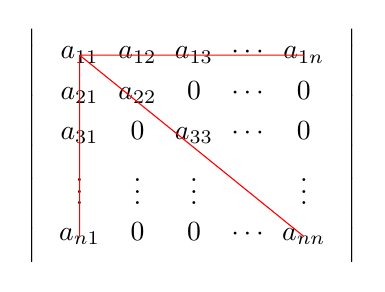
\begin{tikzpicture}
      \matrix(A) [matrix of math nodes,nodes in empty cells,ampersand replacement=\&,left delimiter=|,right delimiter=|] {
        a_{11} \& a_{12} \& a_{13} \& \cd \& a_{1n} \\
        a_{21} \& a_{22} \& 0     \& \cd \&  0    \\
        a_{31} \&  0    \& a_{33} \& \cd \&  0    \\
        \vd  \&  \vd  \&  \vd  \&     \&  \vd  \\
        a_{n1} \&  0    \& 0 \& \cd \& a_{nn} \\
      };
      \draw[red] (A-1-1.center) -- (A-1-5.center) (A-1-1.center) -- (A-5-1.center) (A-1-1.center) -- (A-5-5.center);
    \end{tikzpicture}
  \end{center}
  \pause 
  其解法固定,即从第二行开始,每行依次乘一个系数然后加到第一行,使得第一行除第一个元素外都为零,从而得到一个下三角行列式。
  
  \pause\vspace{0.1in}

  类似的方式还可用于求解如下形式的“爪型行列式”
  \begin{figure}
    \centering
    \subfigure[]{
      
\begin{tikzpicture}
        \matrix(B) [matrix of math nodes,nodes in empty cells,ampersand replacement=\&,left delimiter=|,right delimiter=|] {
          \&  \& \\
          \&  \& \\
          \&  \& \\ 
        };
        \draw[red] (B-1-3.north east) -- (B-1-1.north west) 
        (B-1-3.north east) -- (B-3-1.south west) 
        (B-1-3.north east) -- (B-3-3.south east);
      \end{tikzpicture}
    }
    \subfigure[]{
      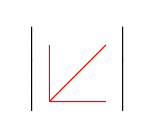
\begin{tikzpicture}
        \matrix(B) [matrix of math nodes,nodes in empty cells,ampersand replacement=\&,left delimiter=|,right delimiter=|] {
          \&  \& \\
          \&  \& \\
          \&  \& \\
        };
        \draw[red]
        (B-3-1.south west) -- (B-1-1.north west) 
        (B-3-1.south west) -- (B-1-3.north east) 
        (B-3-1.south west) -- (B-3-3.south east);
      \end{tikzpicture}
    }
    \subfigure[]{
      
\begin{tikzpicture}
        \matrix(B) [matrix of math nodes,nodes in empty cells,ampersand replacement=\&,left delimiter=|,right delimiter=|] {
          \&  \& \\
          \&  \& \\
          \&  \& \\
        };
        \draw[red]
        (B-3-3.south east) -- (B-1-1.north west) 
        (B-3-3.south east) -- (B-1-3.north east) 
        (B-3-3.south east) -- (B-3-1.south west);
      \end{tikzpicture}
    }
      
    \end{figure}

    \end{itemize}
  
\end{frame}



\begin{frame}
  
    \begin{itemize}
    \item 发散型行列式
      $$
        D_{2n} = \left|
        \begin{array}{cccccc}
          a &     & & & & b \\
          & \dd & & & \id & \\
          &   & a & b &  & \\
          &   & c & d &  &  \\
          & \id & & & \dd & \\
          c &     & & & & d
        \end{array}
        \right|=(ad-bc)^n
        $$        
    \end{itemize}
  
\end{frame}



\begin{frame}
  
    \begin{itemize}
    \item 范德蒙德(Vandermonde)行列式
        $$
        D_n = \left|
        \begin{array}{cccc}
          1        &  1        & \cd &    1     \\                    
          x_1      &  x_2      & \cd &    x_n    \\ 
          x_1^2    &  x_2^2     & \cd &   x_n^2   \\ 
          \vd      &  \vd      &     &    \vd      \\
          x_1^{n-1} & x_2^{n-1} &  \cd &  x_n^{n-1}
        \end{array}
        \right|
        = \prod_{n \ge i > j \ge 1}(x_i-x_j).
        $$
        
        \begin{exampleblock}{常见题型}
        $$
        \left|
        \begin{array}{ccc}
          1   &   1   &   1\\
          a   &   b   &   c\\
          a^3 &   b^3 &   c^3
        \end{array}
        \right|=(a+b+c)(b-a)(c-a)(c-b)
        $$\vspace{0.1in}
        
        $$
        \left|
        \begin{array}{ccc}
          1&a^2&a^3\\
          1&b^2&b^3\\
          1&c^2&c^3
        \end{array}
        \right|=(ab+bc+ca)
        \left|
        \begin{array}{ccc}
          1&a&a^2\\
          1&b&b^2\\
          1&c&c^2
        \end{array}
        \right|
        $$
      \end{exampleblock}

    \end{itemize}
  
\end{frame}

\subsection{往年试题}

\begin{frame}  
    \begin{li}[2005-2006第二学期]
      设$\MA=\left(
      \begin{array}{rrrr}
        1&2&-3&-1\\
        1&-2&1&1\\
        0&1&-1&2\\
        3&0&2&4
      \end{array}
      \right)$,求$|\MA\MA^T|$。
    \end{li}
    \pause

    \begin{jie}
    因
    $\red{
    |\MA\MA^T|=|\MA|~|\MA^T|=|\MA|^2}
    $,而
    $$
    \begin{array}{rl}
      |\MA|&=\left|
      \begin{array}{rrrr}
        1&2&-3&-1\\
        0&-4&4&2\\
        0&1&-1&2\\
        0&-6&11&7
      \end{array}
      \right|=\left|
      \begin{array}{rrr}
        -4&4&2\\
        1&-1&2\\
        -6&11&7
      \end{array}
      \right|\\[0.3in]
      &=\left|
      \begin{array}{rrr}
        -4&0&2\\
        1&0&2\\
        -6&5&7
      \end{array}
      \right|=-5\left|
      \begin{array}{rrr}
        -4&2\\
        1&2\\
      \end{array}
      \right|=50
    \end{array}
    $$
    故$$|\MA\MA^T|=2500$$
  \end{jie}
\end{frame}


\begin{frame}
  
    \begin{li}[2009-2010第二学期]
      设$\MA=\left(
      \begin{array}{rrr}
        1&2&3\\
        4&5&6\\
        7&8&9\\
        10&11&12
      \end{array}
      \right)$,求$|\MA\MA^T|$。
    \end{li}
    \pause

    \begin{jie}
    因$\red{\rank(\MA\MA^T)\le \rank(\MA)\le 3}$,故$\MA\MA^T$为降秩矩阵,从而$|\MA\MA^T|=0$。
    \end{jie}
\end{frame}


\begin{frame}
  
    \begin{li}[2006-2007第一学期]
      设$\MA=(a_{ij})$为$2007$阶方阵,其中$a_{ij}=i-j$,求$|\MA|$
    \end{li}
    \pause
    \begin{jie}
    注意到
    $$
    a_{ij}=i-j=-(j-i)=-a_{ji},
    $$
    故$\MA$为反对称矩阵,由\red{奇数阶反对称矩阵的行列式为零}可知,$$|\MA|=0.$$
    \end{jie}
\end{frame}



\begin{frame}
  
    \begin{li}[2006-2007第二学期]
      计算
      $$
      D=\left|
      \begin{array}{rrrrrr}
        1&2&3&\cd&n-1&n\\
        -1&0&3&\cd&n-1&n\\
        -1&-2&0&\cd&n-1&n\\
        \vd&\vd&\vd&\dd&\vd&\vd\\
        -1&-2&-3&\cd&-(n-1)&0
      \end{array}
      \right|~~(n\ge 1)
      $$
    \end{li}
    \pause 
    \begin{jie}
    $$
    D\xlongequal[\ds i=2,\cd,n]{\ds r_i+r_1}\left|
      \begin{array}{rrrrrr}
        1&2&3&\cd&n-1&n\\
        0&2&6&\cd&2(n-1)&2n\\
        0&0&3&\cd&2(n-1)&2n\\
        \vd&\vd&\vd&\dd&\vd&\vd\\
        0&0&0&\cd&0&n
      \end{array}
      \right|=n!
    $$
    \end{jie}
\end{frame}

\begin{frame}
  
    \begin{li}[2006-2007第二学期]
      计算
      $$
      D=\left|
      \begin{array}{rrrrrr}
        1&2&3&\cd&n-1&n\\
        2&3&4&\cd&n&n+1\\
        3&4&5&\cd&n+1&n+2\\
        \vd&\vd&\vd&\dd&\vd&\vd\\
        n&n+1&n+2&\cd&2n-2&2n-1
      \end{array}
      \right|
      $$
    \end{li}
    \pause

    \begin{jie}
    $$
    \begin{array}{rl}
      D&\xlongequal[i=n,n-1,\cd,2]{\ds r_{i}-r_{i-1}}\left|
      \begin{array}{rrrrrr}
        1&2&3&\cd&n-1&n\\
        1&1&1&\cd&1&1\\
        1&1&1&\cd&1&1\\
        \vd&\vd&\vd&\dd&\vd&\vd\\
        1&1&1&\cd&1&1
      \end{array}
      \right|=0
    \end{array}
    $$
    \end{jie}
    
\end{frame}


\begin{frame}
  
    \begin{li}[2007-2008第一学期,2010-2011第二学期,2011-2012第一学期]
      计算
      $
      D=\left|
      \begin{array}{rrrrr}
        x+a_1&a_2&a_3&\cd&a_n\\
        a_1&x+a_2&a_3&\cd&a_n\\
        a_1&a_2&x+a_3&\cd&a_n\\
        \vd&\vd&\vd&\dd&\vd\\
        a_1&a_2&a_3&\cd&x+a_n
      \end{array}
      \right|
      $
    \end{li}
    

    \pause
    \begin{small}
    \begin{jie}[加边法]
    \begin{itemize}
    \item 当$x=0$时,$D=0$
    \item 当$x\ne 0$时,
      $$
    \begin{array}{rl}
            D&=\left|
      \begin{array}{rrrrrr}
        1&a_1&a_2&a_3&\cd&a_n\\
        0&x+a_1&a_2&a_3&\cd&a_n\\
        0&a_1&x+a_2&a_3&\cd&a_n\\
        0&a_1&a_2&x+a_3&\cd&a_n\\
        \vd&\vd&\vd&\vd&\dd&\vd\\
        0&a_1&a_2&a_3&\cd&x+a_n
      \end{array}      \right|=\left|
      \begin{array}{rrrrrr}
        1&a_1&a_2&a_3&\cd&a_n\\
        -1&x&0&0&\cd&0\\
        -1&0&x&0&\cd&0\\
        -1&0&0&x&\cd&0\\
        \vd&\vd&\vd&\vd&\dd&\vd\\
        -1&0&0&0&\cd&x
      \end{array}
      \right|\\[0.4in]
      &\xlongequal[]{r_1-\frac{a_1}xr_2-\cd--\frac{a_n}xr_{n+1}}
      \left|
      \begin{array}{rrrrrr}
        1+\frac{a_1+a_2+\cd+a_n}x&0&0&0&\cd&0\\
        -1&x&0&0&\cd&0\\
        -1&0&x&0&\cd&0\\
        -1&0&0&x&\cd&0\\
        \vd&\vd&\vd&\vd&\dd&\vd\\
        -1&0&0&0&\cd&x
      \end{array}
      \right|=\ds x^{n-1}(x+\sum_{i=1}^na_i)
    \end{array}
      $$
    \end{itemize}
  \end{jie}
  \end{small}
\end{frame}


\begin{frame}
  
    \begin{li}[2008-2009第一学期]
      计算$
      D=\left|
      \begin{array}{ccccc}
        a_1-b&a_2&a_3&\cd&a_n\\
        a_1&a_2-b&a_3&\cd&a_n\\
        a_1&a_2&a_3-b&\cd&a_n\\
        \vd&\vd&\vd&\dd&\vd\\
        a_1&a_2&a_3&\cd&a_n-b
      \end{array}
      \right|
      $
    \end{li}
  
\end{frame}

\begin{frame}
  
    \begin{li}[2011-2012第二学期]
      计算
      $
      D=\left|
      \begin{array}{cccccc}
        x&1&2&\cd&8&9\\
        1&x&2&\cd&8&9\\
        1&2&x&\cd&8&9\\
        \vd&\vd&\vd&\dd&\vd&\vd\\
        1&2&3&\cd&x&9\\
        1&2&3&\cd&9&x
      \end{array}
      \right|
      $
    \end{li}
    
    \pause
    \begin{small}
    \begin{jie}
    $$
    \begin{array}{rl}
      D&=(x+45)\left|
    \begin{array}{cccccc}
      1&1&2&\cd&8&9\\
      1&x&2&\cd&8&9\\
      1&2&x&\cd&8&9\\
      \vd&\vd&\vd&\dd&\vd&\vd\\
      1&2&3&\cd&x&9\\
      1&2&3&\cd&9&x
      \end{array}
    \right|=(x+45)\left|
    \begin{array}{cccccc}
      1&1&2&\cd&8&9\\
      0&x-1&0&\cd&0&0\\
      0&1&x-2&\cd&0&0\\
      \vd&\vd&\vd&\dd&\vd&\vd\\
      0&1&1&\cd&x-8&0\\
      0&1&1&\cd&1&x-9
      \end{array}
    \right|\\[0.4in]
    &=(x+45)\left|
    \begin{array}{cccccc}      
      x-1&0&\cd&0&0\\
      1&x-2&\cd&0&0\\
      \vd&\vd&\dd&\vd&\vd\\
      1&1&\cd&x-8&0\\
      1&1&\cd&1&x-9
      \end{array}
    \right|=(x+45)(x-1)(x-2)\cd(x-9)
    \end{array}
    $$
  \end{jie}
  \end{small}
\end{frame}

\begin{frame}
  
    \begin{li}[2012-2013第二学期]
      计算
      $$
      \left|
      \begin{array}{ccccc}
        4&3&\cd&3&3\\
        3&4&\cd&3&3\\
        \vd&\vd&\dd&\vd&\vd\\
        3&3&\cd&4&3\\
        3&3&\cd&3&4
      \end{array}
      \right|
      $$
    \end{li}
    \pause

    \begin{jie}
      可用加边法
    \end{jie}
  
\end{frame}


\begin{frame}
  
    \begin{li}[2007-2008第一学期,2010-2011第一学期]
      设$\alphabd_1,\alphabd_2,\alphabd_3,\betabd_1,\betabd_2$都是四维列向量,且四阶行列式
      $$
      |\alphabd_1,\alphabd_2,\alphabd_3,\betabd_1|=m,~~
      |\alphabd_1,\alphabd_2,\betabd_2,\alphabd_3|=n,      
      $$
      求四阶行列式$|\alphabd_1,\alphabd_2,\alphabd_3,\betabd_1+\betabd_2|$
    \end{li}
    \pause

    \begin{jie}
    $$
    \begin{array}{rl}
      |\alphabd_1,\alphabd_2,\alphabd_3,\betabd_1+\betabd_2|&=
      |\alphabd_1,\alphabd_2,\alphabd_3,\betabd_1|+
      |\alphabd_1,\alphabd_2,\alphabd_3,\betabd_2|\\[0.1in]
      &=
      |\alphabd_1,\alphabd_2,\alphabd_3,\betabd_1|-
      |\alphabd_1,\alphabd_2,\betabd_2,\alphabd_3|=m-n
    \end{array}
    $$
  \end{jie}
\end{frame}


\begin{frame}
  
    \begin{li}[2007-2008第二学期]
      设$\alphabd_1,\alphabd_2,\alphabd_3$都是三维列向量,记三阶矩阵
      $$
      \MA=(\alphabd_1,\alphabd_2,\alphabd_3),~~
      \MB=(\alphabd_1+\alphabd_2+\alphabd_3,\alphabd_1+2\alphabd_2+4\alphabd_3,\alphabd_1+3\alphabd_2+9\alphabd_3),
      $$已知$|\MA|=1$,求$|\MB|$。
    \end{li}
    \pause

    \begin{jie}
    因
    $$
    \MB=(\alphabd_1,\alphabd_2,\alphabd_3)\left(
    \begin{array}{ccc}
      1&1&1\\
      1&2&3\\
      1&4&9
    \end{array}
    \right)=\MA\left(
    \begin{array}{ccc}
      1&1&1\\
      1&2&3\\
      1&4&9
    \end{array}
    \right)
    $$
    而
    $$
    \left|
    \begin{array}{ccc}
      1&1&1\\
      1&2&3\\
      1&4&9
    \end{array}
    \right|=\left|
    \begin{array}{ccc}
      1&1&1\\
      0&1&2\\
      0&3&8
    \end{array}
    \right|=\left|
    \begin{array}{ccc}
      1&1&1\\
      0&1&2\\
      0&0&2
    \end{array}
    \right|=2    
    $$
    故$$|\MB|=2|\MA|=2.$$
  \end{jie}
\end{frame}


\begin{frame}
  
    \begin{li}[2008-2009第一学期]
      计算
      $
      D=\left|
      \begin{array}{rrr}
        -ab&ac&ae\\
        bd&-cd&de\\
        bf&cf&-cf
      \end{array}
      \right|
      $
    \end{li}
    \pause

    \begin{jie}
    $$
    \begin{array}{rl}
    D&=adf\left|
      \begin{array}{rrr}
        -b&c&e\\
        b&-c&e\\
        b&c&-c
      \end{array}
      \right|=adf\left|
      \begin{array}{rrr}
        -b&c&e\\
        0&0&2e\\
        0&2c&e-c
      \end{array}
      \right|\\[0.2in]
      &=-adf\left|
      \begin{array}{rrr}
        -b&c&e\\
        0&2c&e-c\\
        0&0&2e
      \end{array}
      \right|  
      =-adf\cdot(-b)\cdot 2c \cdot 2e=4abcdef
    \end{array}
    $$
    \end{jie}
\end{frame}




\begin{frame}
  
    \begin{li}[2012-2013第二学期]
      计算
      $
      D=\left|
      \begin{array}{rrrr}
        1&2&0&0\\
        -1&1&0&0\\
        0&-1&-2&4\\
        0&0&-1&-3
      \end{array}
      \right|
      $
    \end{li}
    \pause

    \begin{jie}
    $$
    D=\left|
    \begin{array}{rr}
      1&2\\
      -1&1
    \end{array}
    \right|\left|
    \begin{array}{rr}
      -2&4\\
      -1&-3
    \end{array}
    \right|=3\cdot10=30
    $$
    \end{jie}
\end{frame}


\begin{frame}
  
    \begin{li}[2013-2014第一学期]
      在$n$阶行列式$D$中,如果把第一列移到最后一列,而其余各列保持原来次序各向左移动了一列,得到行列式$\Delta$,问$\Delta$与$D$有何关系?
    \end{li}
    \pause

    \begin{jie}
    $$
    \Delta=(-1)^{n-1}D
    $$
  \end{jie}
  
\end{frame}




\section{矩阵及其运算}

\subsection{往年试题}
\begin{frame}

\begin{li}[2005-2006第一学期]
已知$\MA$为$n(n\ge 2)$矩阵,且$\MA$非奇异,求$(\MA^*)^*$。
\end{li}
\pause
\begin{jie}
由$\MA^{-1}=\MA^*/|\MA|$,可知$\MA^*=|\MA|\MA^{-1}$,从而$|\MA^*|=|\MA|^{n-1}$。
而
$$
(\MA^*)^*=|\MA^*|(\MA^*)^{-1}=|\MA|^{n-1}(|\MA|\MA^{-1})^{-1}=|\MA|^{n-2}\MA.
$$
\end{jie}
\end{frame}

\begin{frame}

\begin{li}[2005-2006第一学期, 2009-2010第一学期, 2010-2011第一学期, 2011-2012第一学期]
设$\MA=\left(
\begin{array}{rrr}
1&0&1\\
0&2&0\\
1&6&a
\end{array}
\right)$,且$\rank(\MA)=2$,$\MX$满足$\MA\MX+\MI=\MA^2+\MX$,求$a$和$\MX$。
\end{li}
\pause

\begin{jie}
因$\MA \rightarrow \left(
\begin{array}{ccc}
1&0&1\\
0&2&0\\
0&0&a-1
\end{array}
\right)$,
由$\rank(\MA)=2$知$a=1$,故$\MA=\left(
\begin{array}{rrr}
1&0&1\\
0&2&0\\
1&6&1
\end{array}
\right)$.
\vspace{0.1in}


$$\blue{
\MA\MX+\MI=\MA^2+\MX ~~\Rightarrow~~
(\MA-\MI)\MX=\MA^2-\MI=(\MA-\MI)(\MA+\MI)
}
$$
因$
\MA-\MI=\left(
\begin{array}{rrr}
0&0&1\\
0&1&0\\
1&6&0
\end{array}
\right)
$可逆,故
$$
\MX=\MA+\MI=\left(
\begin{array}{rrr}
2&0&1\\
0&3&0\\
1&6&2
\end{array}
\right)
$$
\end{jie}
\end{frame}

\begin{frame}

\begin{li}[2005-2006第一学期]
设$\MA$为$n$阶实矩阵,
\begin{itemize}
\item[(1)] 当$n$为奇数且$\MA\MA^T=\MI$及$|\MA|=1$时,证明$|\MI-\MA|=0$;
\item[(2)]  当$m$为任意给定正整数且$(\MA+\MI)^m=\M0$,证明$\MA$可逆。
\end{itemize}
\end{li}
\pause
\begin{proof}
\begin{itemize}
\item[(1)]
由$\MA\MA^T=\MI$知$A^T=\MA^{-1}$。
又$\MI-\MA=(\MA^{-1}-\MI)\MA=(\MA^T-\MI)\MA$,故
$$
|\MI-\MA|=|\MA^T-\MI||\MA|=|\MA-\MI|=(-1)^n=|\MI-\MA|
$$
而$n$为奇数,于是
$
|\MI-\MA|=-|\MI-\MA|
$,即$|\MI-\MA|=0$。\\[0.1in] \pause 
\item[(2)]
由$(\MA+\MI)^m=\M0$,即$\MA^m+C_m^{m-1}\MA^{m-1}+\cd++C_m^{1}\MA+\MI=\M0$可知,
$$
\MA(\MA^{m-1}+C_m^{m-1}\MA^{m-2}+\cd+C_m^{1}\MI)=-\MI
$$
故
$$
\MA^{-1}=-(\MA^{m-1}+C_m^{m-1}\MA^{m-2}+\cd+C_m^{1}\MI).
$$
\end{itemize}
\end{proof}
\end{frame}


\begin{frame}

\begin{li}[2005-2006第二学期]
设$\MA=\left(
\begin{array}{rrr}
1&1&-1\\
0&1&1\\
0&0&-1
\end{array}
\right)$,且$\MA^2-\MA\MB=\MI$,
\begin{itemize}
\item[(1)] 求$\MB$;
\item[(2)]  令$\MC=4\MA^2-\MB^2-2\MB\MA+2\MA\MB$,计算$\MC^*$。
\end{itemize}
\end{li}
\pause

\begin{jie}
\begin{itemize}
\item[(1)]
由$\MA^2-\MA\MB=\MI$知$\MA\MB=\MA^2-\MI$。利用如下过程可求得$\MB$:
$$\boxed{\blue{
(\MA, ~~\MA^2-\MI) ~~\xlongrightarrow[]{\mbox{初等行变换}} (\MI, ~~\MB)
}
}
$$
易求得$\MA^2-\MI=\left(
\begin{array}{rrr}
0&2&1\\
0&0&0\\
0&0&0
\end{array}
\right)$,故
$$\left(
\begin{array}{rrrrrr}
1&1&-1&0&2&1\\
0&1&1&0&0&0\\
0&0&-1&0&0&0
\end{array}
\right) \longrightarrow
\left(
\begin{array}{rrrrrr}
1&0&0&0&2&1\\
0&1&0&0&0&0\\
0&0&1&0&0&0
\end{array}
\right)
$$
\end{itemize}
\end{jie}
\end{frame}

\begin{frame}

\begin{itemize}
\item[(2)]
易求得
$$
\MC=(2\MA-\MB)(2\MA+\MB)=\left(
\begin{array}{rrr}
4&8&4\\
0&4&0\\
0&0&4
\end{array}
\right) $$
故
$$
\MC^{-1}=\frac14\left(
\begin{array}{rrr}
1&-2&-1\\
0&1&0\\
0&0&1
\end{array}
\right), \quad |\MC|=64.
$$
故
$$
\MC^*=|\MC|\MC^{-1}=16\left(
\begin{array}{rrr}
1&-2&-1\\
0&1&0\\
0&0&1
\end{array}
\right)
$$
\end{itemize}•

\end{frame}




\begin{frame}

\begin{li}[2006-2007第一学期]
设三阶方阵$\MA=(a_{ij})$,
\begin{itemize}
\item[(1)] 若$\MA^T=\MA$且$\MA^2=\M0$,证明$\MA=\M0$;并由反例说明一般情况下$\MA^2=\M0$得不出$\MA=\M0$;
\item[(2)]  若$\MA$可逆,将其第二行的$2$倍加到第三行的矩阵为$\MB$,问$\MB\MA^{-1}-\MA\MB^{-1}$是否可逆?
\end{itemize}
\end{li}
\pause

\begin{jie}
\begin{itemize}
\item[(1)]
由条件知$\MA^T\MA=\M0$,而$(\MA^T\MA)_{ii}=a_{1i}^2+a_{2i}^2+\cd+a_{ni}^2=0$,故$a_{ij}=0$,即$\MA=\M0$。
反例:$\MA=\left(\begin{array}{cc}
0&1\\0&0
\end{array}\right)\ne \M0$,但$\MA^2=\left(\begin{array}{cc}
0&0\\0&0
\end{array}\right)$. \pause
\item[(2)]
由题意知$\MB=\MP\MA$,其中$\MP=\left(\begin{array}{ccc}
1&&\\0&1&\\0&3&1
\end{array}\right)$. 故
$$
\begin{array}{rl}
\MB\MA^{-1}-\MA\MB^{-1}&=\MP\MA\MA^{-1}-\MA\MA^{-1}\MP^{-1}=\MP-\MP^{-1} \\[0.1in]
&=\left(\begin{array}{ccc}
1&&\\0&1&\\0&3&1
\end{array}\right)-\left(\begin{array}{ccc}
1&&\\0&1&\\0&-3&1
\end{array}\right)=\left(\begin{array}{ccc}
0&&\\0&0&\\0&6&0
\end{array}\right),
\end{array}
$$ 显然不可逆。
\end{itemize}
\end{jie}

\end{frame}

\begin{frame}

\begin{li}[2006-2007第二学期]
设$\MA=\left(
\begin{array}{rrr}
1&2&1\\
2&1&1\\
1&1&2
\end{array}
\right)$, $\MB=\left(
\begin{array}{rrr}
-1&1&0\\
1&3&1\\
-1&0&1
\end{array}
\right)$,
\begin{itemize}
\item[(1)] 求$(\MA+\MB)^2-(\MA^2+2\MA\MB+\MB^2)$;
\item[(2)]  求$\MA^{-1}$。
\end{itemize}
\end{li}
\pause

\begin{jie}
\begin{itemize}
\item[(1)]  $(\MA+\MB)^2-(\MA^2+2\MA\MB+\MB^2)=\MB\MA-\MA\MB=\left(
\begin{array}{rrr}
1&-1&0\\
8&6&6\\
0&-1&1
\end{array}
\right)-\left(
\begin{array}{rrr}
0&7&3\\
-2&5&2\\
-2&4&3
\end{array}
\right)=\left(
\begin{array}{rrr}
1&-8&-3\\
10&1&4\\
2&-5&-2
\end{array}
\right)$ \pause 
\item[(2)]
$$
\begin{array}{rl}
(\MA,~\MI)&=\left(
\begin{array}{rrrrrr}
1&2&1&1&0&0\\
2&1&1&0&1&0\\
1&1&2&0&0&1
\end{array}
\right)\rightarrow\left(
\begin{array}{rrrrrr}
1&2&1&1&0&0\\
0&-3&-1&-2&1&0\\
0&-1&1&-1&0&1
\end{array}
\right)\\
&\rightarrow\left(
\begin{array}{rrrrrr}
1&2&1&1&0&0\\
0&1&-1&1&0&-1\\
0&0&-4&1&1&-3\\
\end{array}
\right)\rightarrow\left(
\begin{array}{rrrrrr}
1&0&0&-\frac14&\frac34&-\frac14\\
0&1&0&\frac34&-\frac14&-\frac14\\
0&0&1&-\frac14&-\frac14&\frac34\\
\end{array}
\right)
\end{array}
$$
\end{itemize}
\end{jie}
\end{frame}

\begin{frame}

\begin{li}[2006-2007第二学期]
设$\MA=\left(
\begin{array}{rrr}
1&-3&2\\
-2&1&-1\\
1&2&-1
\end{array}
\right)$, $\MB=\left(
\begin{array}{rrr}
2&5&4\\
4&-2&2\\
1&4&1
\end{array}
\right)$,
\begin{itemize}
\item[(1)] 求$4\MA^2-\MB^2-2\MB\MA+2\MA\MB$;
\item[(2)]  求$|\MA^*|$。
\end{itemize}
\end{li}
\pause

\begin{jie}
\begin{itemize}
\item[(1)] $4\MA^2-\MB^2-2\MB\MA+2\MA\MB=(2\MA-\MB)(2\MA+\MB)=\left(
\begin{array}{rrr}
0&0&0\\
-44&-24&-60\\
-5&-25&11
\end{array}
\right)$ \pause 
\item[(2)]  因$|\MA^*|=|\MA|^{2}$,而
$
|\MA|=\left|
\begin{array}{rrr}
1&-3&2\\
0&-5&3\\
0&5&-3
\end{array}
\right|=0
$,
故$|\MA^*|=0$。
\end{itemize}
\end{jie}
\end{frame}

\begin{frame}

\begin{li}[2007-2008第一学期]
证明
\begin{itemize}
\item[(1)] 设$\MA$为$n$阶方阵,证明:若$|\MA|=0$,则$|\MA^*|=0$;
\item[(2)]  设$\MA,\MB$为$n$阶方阵,且满足$\MA^2=\MA,\MB^2=\MB,\rank(\MA+\MB-\MI)=n$,证明:$\rank(\MA)=\rank(\MB)$。
\end{itemize}
\end{li}
\pause

\begin{proof}
\begin{itemize}
\item[(1)] $|\MA^*|=|\MA|^{n-1}=0$;\pause 
\item[(2)]  由$\rank(\MA+\MB-\MI)=n$知$\MA+\MB-\MI$可逆。故
$$
\rank(\MA)=\rank(\MA(\MA+\MB-\MI))=\rank(\MA\MB)
$$
$$
\rank(\MB)=\rank((\MA+\MB-\MI)\MB)=\rank(\MA\MB)
$$
于是$\rank(\MA)=\rank(\MB)$.
\end{itemize}
\end{proof}
\end{frame}


\begin{frame}
\begin{li}[2007-2008第二学期]
设$\MA=\left(
\begin{array}{rrr}
2&-1&1\\
1&2&0\\
2&1&2
\end{array}
\right)$, $\MB=\left(
\begin{array}{rrr}
0&2&-3\\
2&-1&4\\
0&-1&4
\end{array}
\right)$,$\MA\MC-\MI=\MB+\MC$,求$\MC$。
\end{li}
\pause

\begin{jie}
由题意可知$(\MA-\MI)\MC=\MB+\MI$,
$$
\begin{array}{rl}
&(\MA-\MI,\MB+\MI)=\left(
\begin{array}{rrrrrr}
1&-1&1 &1&2&-3\\
1&1&0 &2&0&4\\
2&1&1&0&-1&5
\end{array}
\right)\rightarrow\left(
\begin{array}{rrrrrr}
1&-1&1 &1&2&-3\\
0&2&-1 &1&-2&7\\
0&3&-1&-2&-5&11
\end{array}
\right)\\[0.2in]
&\rightarrow\left(
\begin{array}{rrrrrr}
1&-1&1 &1&2&-3\\
0&2&-1 &1&-2&7\\
0&0&1&-7&-4&1
\end{array}
\right) \rightarrow\left(
\begin{array}{rrrrrr}
1&-1&0 &8&6&-4\\
0&1&0 &-3&-3&4\\
0&0&1&-7&-4&1
\end{array}
\right)\\[0.2in]
& \rightarrow\left(
\begin{array}{rrrrrr}
1&-1&0 &8&6&-4\\
0&1&0 &-3&-3&4\\
0&0&1&-7&-4&1
\end{array}
\right) \rightarrow\left(
\begin{array}{rrrrrr}
1&0&0 &5&3&0\\
0&1&0 &-3&-3&4\\
0&0&1&-7&-4&1
\end{array}
\right)
\end{array}
$$
\end{jie}
\end{frame}


\begin{frame}

\begin{li}[2008-2009第一学期]
设$\MA,\MB$为三阶方阵,满足$\MA\MB+\MI=\MA^2+\MB$,且$\MA=\left(
\begin{array}{rrr}
1&0&1\\
0&2&0\\
1&0&1
\end{array}
\right)$, 求$\MB$及$\MB^*$。
\end{li}
\pause

\begin{jie}
依题意可知
$$
(\MA-\MI)\MB=\MA^2-\MI=(\MA-\MI)(\MA+\MI),
$$
而$\MA-\MI=\left(
\begin{array}{rrr}
0&0&1\\
0&2&0\\
1&0&0
\end{array}
\right)$非奇异,故$$\MB=\MA+\MI=\left(
\begin{array}{rrr}
2&0&1\\
0&3&0\\
1&0&2
\end{array}
\right)$$
\end{jie}
\end{frame}






\begin{frame}

\begin{li}[2009-2010第一学期]
计算下列各题:
\begin{itemize}
\item[(1)] 已知$\MA=\left(
\begin{array}{rrr}
a&a&a\\
b&b&b\\
c&c&c
\end{array}
\right)$,求$\MA^{2010}$;
\item[(2)] 设$n(n\ge2)$阶方阵$\MA$非奇异,求$(\MA^*)^*$。
\end{itemize}
\end{li}
\pause

\begin{jie}
\begin{itemize}
\item[(1)]由$|\MA-\lambda\MI|
%=\left|
%\begin{array}{rrr}
%a-\lambda&a&a\\
%b&b-\lambda&b\\
%c&c&c-\lambda
%\end{array}
%\right|
%=(a+b+c-\lambda)\left|
%\begin{array}{rrr}
%1&1&1\\
%b&b-\lambda&b\\
%c&c&c-\lambda
%\end{array}
%\right|=(a+b+c-\lambda)\left|
%\begin{array}{rrr}
%1&0&0\\
%b&-\lambda&\\
%c&0&-\lambda
%\end{array}
%\right|
=(a+b+c-\lambda)\lambda^2=0$知,
特征值为$\lambda_{1,2}=0$与$\lambda_3=a+b+c$。
\begin{itemize}
\item
$\lambda_{1,2}=0$,方程为$x+y+z=0$,基础解系为$\boxed{\vx_1=(-1,1,0)^T,\vx_2=(-1,0,1)^T}$。\\[0.1in]
\item
$\lambda_3=a+b+c$,方程为$\left(
\begin{array}{rrr}
-b-c&a&a\\
b&-a-c&b\\
c&c&-a-b
\end{array}
\right)\vx=\M0$,基础解系为$\boxed{\vx_3=(a,b,c)^T}$。
\end{itemize}
\end{itemize}
\end{jie}
\end{frame}

\begin{frame}

故
$$
\MA(\vx_1,\vx_2,\vx_3)=(\vx_1,\vx_2,\vx_3)\left(
\begin{array}{ccc}
0&&\\
&0&\\
&&a+b+c
\end{array}
\right)
$$
从而
$$
\MA^{2010}=\MP\left(
\begin{array}{ccc}
0&&\\
&0&\\
&&a+b+c
\end{array}
\right)^{2010}\MP^{-1}
$$
其中
$$
\MP=\left(
\begin{array}{ccc}
-1&-1&a\\
1&0&b\\
0&1&c
\end{array}
\right), \quad
\MP^{-1}=\frac1{a+b+c}\left(
\begin{array}{ccc}
-b&a+c&-b\\
-c&-c&a+b\\
1&1&1
\end{array}
\right)
$$
故
$$
\MA^{2010}= (a+b+c)^{2009}
\left(
\begin{array}{ccc}
a&a&a\\
b&b&b\\
c&c&c
\end{array}
\right)
$$

\end{frame}

\begin{frame}

\begin{li}[2009-2010第一学期,2011-2012第二学期]
设三阶方阵$\MA$满足$\MA\MX=\MA+2\MX$,且$\MA=\left(
\begin{array}{rrr}
3&0&1\\
1&1&0\\
0&1&4
\end{array}
\right)$,求$\MX$。
\end{li}
\pause
\begin{jie}
依题意可知$(\MA-2\MI)\MX=\MA$,解此矩阵方程即可求得$\MX$。\pause 
$$
\begin{array}{rl}
&(\MA-2\MI, \MA)=\left(
\begin{array}{rrrrrr}
  1&0&1&3&0&1\\
  1&-1&0&1&1&0\\
  0&1&2&0&1&4
\end{array}
\right)\rightarrow\left(
\begin{array}{rrrrrr}
  1&0&1&3&0&1\\
  0&-1&-1&-2&1&-1\\
  0&1&2&0&1&4
\end{array}
\right)\\[0.2in]
&\rightarrow\left(
\begin{array}{rrrrrr}
  1&0&1&3&0&1\\
  0&-1&-1&-2&1&-1\\
  0&0&1&-2&2&3
\end{array}
\right)\rightarrow\left(
\begin{array}{rrrrrr}
  1&0&1&3&0&1\\
  0&1&0&4&-3&-2\\
  0&0&1&-2&2&3
\end{array}
\right)\\[0.2in]
&\rightarrow\left(
\begin{array}{rrrrrr}
  1&0&0&5&-2&-2\\
  0&1&0&4&-3&-2\\
  0&0&1&-2&2&3
\end{array}
\right)
\end{array}
$$
\end{jie}
\end{frame}


\begin{frame}
\begin{li}[2009-2010第二学期]
已知矩阵方程满足$(2\MI-\MC^{-1}\MB)\MA^T=\MC^{-1}$,求$\MA$,其中
$$\MB=\left(
\begin{array}{rrrr}
1&2&-3&-2\\
0&1&2&-3\\
0&0&1&2\\
0&0&0&1
\end{array}
\right),\quad
\MC=\left(
\begin{array}{rrrr}
1&2&0&1\\
0&1&2&0\\
0&0&1&2\\
0&0&0&1
\end{array}
\right)$$
\end{li}
\pause

\begin{jie}
依题意知$\MA^T=(2\MI-\MC^{-1}\MB)^{-1}\MC^{-1}=(\MC(2\MI-\MC^{-1}\MB))^{-1}=(2\MC-\MB)^{-1}$
$$
\begin{array}{l}
  (2\MC-\MB,~\MI)=\left(
  \begin{array}{rrrrrrrr}
    1&2&3&4&1&0&0&0\\
    0&1&2&3&0&1&0&0\\
    0&0&1&2&0&0&1&0\\
    0&0&0&1&0&0&0&1
  \end{array}
  \right)\rightarrow\left(
  \begin{array}{rrrrrrrr}
    1&2&3&0&1&0&0&-4\\
    0&1&2&0&0&1&0&-3\\
    0&0&1&0&0&0&1&-2\\
    0&0&0&1&0&0&0&1
  \end{array}
  \right)\\[0.3in]
\rightarrow\left(
  \begin{array}{rrrrrrrr}
    1&2&0&0&1&0&-3&2\\
    0&1&0&0&0&1&-2&1\\
    0&0&1&0&0&0&1&-2\\
    0&0&0&1&0&0&0&1
  \end{array}
  \right)
\rightarrow\left(
  \begin{array}{rrrrrrrr}
    1&0&0&0&1&-2&1&0\\
    0&1&0&0&0&1&-2&1\\
    0&0&1&0&0&0&1&-2\\
    0&0&0&1&0&0&0&1   
  \end{array}
  \right)\\[0.3in]
  \red{\Longrightarrow \MA=\left(
  \begin{array}{rrrr}
    1&0&0&0\\
    -2&1&0&0\\
    1&-2&1&0\\
    0&1&-2&1   
  \end{array}
  \right)
}
\end{array}
$$
\end{jie}

\end{frame}

\begin{frame}

\begin{li}[2012-2013第二学期]
已知$\MA$为三阶矩阵,$\MB=\left(
\begin{array}{rrr}
1&-2&0\\
1&2&0\\
0&0&2
\end{array}
\right)$,且满足$2\MA^{-1}\MB=\MB-4\MI$,$\MI$为三阶单位矩阵,求矩阵$\MA$。
\end{li}
\pause

\begin{jie}
依题意$\MA(\MB-4\MI)=2\MB$,可用$\boxed{\left(
  \begin{array}{c}
    \MB-4\MI\\
    2\MB
  \end{array}
\right)\xlongrightarrow[]{\mbox{初等列变换}} \left(
  \begin{array}{c}
    \MI\\
    \red{\MA}
  \end{array}
\right)}$求$\MA$。
$$
\left(
  \begin{array}{c}
    \MB-4\MI\\
    2\MB
  \end{array}
\right)=\left(
\begin{array}{rrr}
-3&-2&0\\
1&-2&0\\
0&0&-2\\
2&-4&0\\
2&4&0\\
0&0&4
\end{array}
\right)\rightarrow
\left(
\begin{array}{rrr}
3  &1&0\\
-1 &1&0\\
0  &0 &1\\
-2 &2 &0\\
-2 &-2&0\\
0  &0 &-2
\end{array}
\right)\rightarrow
\left(
\begin{array}{rrr}
1 &0  &0\\
0 &1 &0\\
0 &0  &1\\
0 &2 &0\\
-1&-1  &0\\
0 &0  &-2
\end{array}
\right)
$$
\end{jie}
\end{frame}


\begin{frame}

\begin{li}[2012-2013第二学期]
设矩阵$\MA=\left(
\begin{array}{rrr}
-1&0&0\\
 0&1&0\\
 0&1&1
\end{array}
\right)$,矩阵$\MB$满足$\MA^*\MB\MA=2\MB\MA-9\MI$,求$\MB$。
\end{li}
\pause

\begin{jie}
易知$|\MA|=-1$,即$\MA$可逆,由$\MA\MA^*=|\MA|\MI=-\MI$可得
$$
\begin{array}{l}
\MA^*\MB\MA=2\MB\MA-9\MI ~~\Rightarrow~~
\MA\MA^*\MB\MA=\MA(2\MB\MA-9\MI) \\[0.1in]
\Rightarrow~~
-\MB\MA=2\MA\MB\MA-9\MA ~~\Rightarrow~~
-\MB=2\MA\MB-9\MI   ~~\Rightarrow~~
(2\MA+\MI)\MB=9\MI
\end{array}
$$
$$
\begin{array}{l}
(2\MA+\MI, 9\MI)=\left(
\begin{array}{rrrrrr}
  -1   &  0  &   0 &  9&0&0\\
  0    & 3   &  0  &  0&9&0\\
  0    & 2   &  3  &  0&0&9
\end{array}
\right)  \rightarrow
\left(
\begin{array}{rrrrrr}
  1   &  0  &   0 & -9&0&0\\
  0    & 1   &  0  &  0&3&0\\
  0    & 0   &  1  &  0&-2&3
\end{array}
\right)  
\end{array}
$$
\end{jie}
\end{frame}

\begin{frame}

\begin{li}[2012-2013第二学期]
设矩阵$\MA=\left(
\begin{array}{rrrr}
1&-1&-1&-1\\
-1&1&-1&-1\\
-1&-1&1&-1\\
-1&-1&-1&1
\end{array}
\right)$,
\begin{itemize}
\item[(1)] 求$\MA^n$;
\item[(2)] 设$\MA^2+\MA\MB-\MA=\MI$,求$|\MB|$。
\end{itemize}
\end{li}
\pause

\begin{jie}
\begin{itemize}
\item[(1)] 求矩阵的特征值与特征向量。
  $$
  \begin{array}{l}
    |\MA-\lambda\MI|=\left|
    \begin{array}{rrrr}
      1-\lambda&-1&-1&-1\\
      -1&1-\lambda&-1&-1\\
      -1&-1&1-\lambda&-1\\
      -1&-1&-1&1-\lambda
    \end{array}
    \right|
    =(-2-\lambda)\left|
    \begin{array}{rrrr}
      1&-1&-1&-1\\
      1&1-\lambda&-1&-1\\
      1&-1&1-\lambda&-1\\
      1&-1&-1&1-\lambda
    \end{array}
    \right|\\[0.3in]=(-2-\lambda)\left|
    \begin{array}{rrrr}
      1&-1&-1&-1\\
      0&2-\lambda&0&0\\
      0&0& 2-\lambda&0\\
      0&0& 0 &2-\lambda
    \end{array}
    \right|   = (\lambda+2)(\lambda-2)^3
  \end{array}
$$
\end{itemize}
\end{jie}

\end{frame}


\begin{frame}

  \begin{itemize}
  \item 当$\lambda_{1,2,3}=2$时,$(\MA-\lambda\MI)\vx=\M0$为
    $$
    x_1+x_2+x_3+x_4=0
    $$
    基础解系为
    $$
    \vx_1=(-1,1,0,0)^T,~~
    \vx_2=(-1,0,1,0)^T,~~
    \vx_3=(-1,0,0,1)^T.
    $$
    故对应于$\lambda_{1,2,3}=2$的特征向量为$k_1\vx_1+k_2\vx_2+k_3\vx_3, (k_1,k_2,k_3\mbox{不全为零})$;
  \item 当$\lambda_{4}=-2$时,$(\MA-\lambda\MI)\vx=\M0$为
    $$
    \begin{array}{l}
          \left(
    \begin{array}{rrrr}
      3&-1&-1&-1\\
      -1&3&-1&-1\\
      -1&-1&3&-1\\
      -1&-1&-1&3
    \end{array}
    \right) \rightarrow \left(
    \begin{array}{rrrr}
      1&-3&1&1\\
      1&1&-3&1\\
      1&1&1&-3\\
      3&-1&-1&-1
    \end{array}
    \right) \rightarrow \left(
    \begin{array}{rrrr}
      1&-3&1&1\\
      0&4&-4&0\\
      0&4&0&-4\\
      0&8&-4&-4
    \end{array}
    \right) \\[0.2in]
    \rightarrow \left(
    \begin{array}{rrrr}
      1&-3&1&1\\
      0&1&-1&0\\
      0&0&1&-1\\
      0&0&0&0
    \end{array}
    \right)\rightarrow \left(
    \begin{array}{rrrr}
      1&0&0&-1\\
      0&1&0&-1\\
      0&0&1&-1\\
      0&0&0&0
    \end{array}
    \right)
    \end{array}
    $$
    对应方程为
    $$
    \left\{
    \begin{array}{l}
      x_1=x_4\\
      x_2=x_4\\
      x_3=x_4\\
      x_4=x_4
    \end{array}
    \right.
    $$
    基础解系为$$
    \vx_3=(1,1,1,1)^T
    $$
    
  \end{itemize}

\end{frame}

\begin{frame}

  取
  $$
  \MP=(\vx_1,\vx_2,\vx_3,\vx_4)=\left(
  \begin{array}{rrrr}
    -1 & -1& -1&  1 \\
    1  &  0&  0&  1 \\
    0  &  1&  0&  1  \\
    0  &  0&  1&  1 
  \end{array}
  \right), ~~~\MP^{-1}=\frac14 \left(
  \begin{array}{rrrr}
    -1 &   3& -1&  -1 \\
    -1 &  -1&  3&  -1 \\
    -1 &  -1& -1&   3  \\
     1 &   1&  1&   1 
  \end{array}
  \right)
  $$
  则 $\MA\MP=\MP\Lambdabd$,即
  $$
  \MA=\MP\Lambdabd\MP^{-1},
  $$
  从而$$
  \MA^{n}=\MP\Lambdabd^n\MP^{-1}
  =2^n \MP\left(
  \begin{array}{cccc}
    1&&&\\
    &1&&\\
    &&1&\\
    &&&(-1)^n
  \end{array}
  \right)\MP^{-1}
  $$
  当$n$为偶数时,$\MA^n=2^n \MI$
  当$n$为奇数时,$\MA^n=2^n\MP\left(
  \begin{array}{cccc}
    1&&&\\
    &1&&\\
    &&1&\\
    &&&-1
  \end{array}
  \right)\MP^{-1} $
  而
  $
  \MA=2\MP\left(
  \begin{array}{cccc}
    1&&&\\
    &1&&\\
    &&1&\\
    &&&-1
  \end{array}
  \right)\MP^{-1} 
  $
  故
  $
  \MA^n=2^{n-1}\MA
  $。

\end{frame}

\begin{frame}

  \begin{itemize}
  \item[(2)]
    依题意,
    $$
    \MA\MB=\MI-\MA+\MA^2=\MI-\MA+4\MI=-\MA+5\MI
    $$
    故
    $$
    |\MA||\MB|=|-\MA+5\MI|
    $$
    即
    $$
    -16 |\MB| = |\MA-5\MI| =\left|
    \begin{array}{rrrr}
      -4&-1&-1&-1\\
      -1&-4&-1&-1\\
      -1&-1&-4&-1\\
      -1&-1&-1&-4
    \end{array}
    \right| = 189
    $$
    故
    $$
    |\MB|=-\frac{189}{16}.
    $$
  \end{itemize}

\end{frame}

\section{向量组~~ 矩阵的秩}



\subsection{知识点}

\begin{frame}\ft{线性相关性}
  
    设$m\times n$矩阵$\MA$按列分块为
    $$\MA=(\alphabd_1,\alphabd_2,\cd,\alphabd_n),$$
    其中$\alphabd_i(i=1,2,\cd,n)$为$m$维列向量,则线性组合
    $$
    x_1\alphabd_1+x_2\alphabd_2+\cd+x_n\alphabd_n
    $$
    可表示为矩阵形式
    $$ 
    (\alphabd_1,\alphabd_2,\cd,\alphabd_n)\left(
    \begin{array}{c}
      x_1\\x_2\\\vd\\x_n
    \end{array}
    \right)
    $$
  
\end{frame}


\begin{frame}\ft{线性相关性与齐次线性方程组的解}
  
    \begin{jielun}
      向量组$\alphabd_1,\alphabd_2,\cd,\alphabd_n$线性相关,等价于齐次方程组
        $$
        (\alphabd_1,\alphabd_2,\cd,\alphabd_n)\left(
        \begin{array}{c}
          x_1\\x_2\\\vd\\x_n
        \end{array}
        \right)=\M0
        $$
        有非零解,也等价于
        $$
        \rank(\MA)=\rank(\alphabd_1,\alphabd_2,\cd,\alphabd_n)<n=\mbox{矩阵$\MA$的列数}.
        $$
    \end{jielun}

\end{frame}

\begin{frame}\ft{线性相关性与齐次线性方程组的解}
  
    \begin{jielun}
      向量组$\alphabd_1,\alphabd_2,\cd,\alphabd_n$线性无关,等价于齐次方程组
        $$
        (\alphabd_1,\alphabd_2,\cd,\alphabd_n)\left(
        \begin{array}{c}
          x_1\\x_2\\\vd\\x_n
        \end{array}
        \right)=\M0
        $$
        只有零解,也等价于
        $$
        \rank(\MA)=\rank(\alphabd_1,\alphabd_2,\cd,\alphabd_n)=n=\mbox{矩阵$\MA$的列数}.
        $$

      \end{jielun}
  
\end{frame}


\begin{frame}\ft{线性表示与非齐次线性方程组的解}
  
    \begin{jielun}
      向量$\vb$可由$\alphabd_1,\alphabd_2,\cd,\alphabd_n$线性表示,等价于方程组
      $$
      (\alphabd_1,\alphabd_2,\cd,\alphabd_n)\left(
        \begin{array}{c}
          x_1\\x_2\\\vd\\x_n
        \end{array}
        \right)=\vb
      $$
      有解,也等价于
      $$
      \rank(\MA,\vb)=\rank(\MA).
      $$ 
    \end{jielun}
  
\end{frame}


\begin{frame}\ft{线性表示与非齐次线性方程组的解}
  

    \begin{jielun}
      向量$\vb$可由$\alphabd_1,\alphabd_2,\cd,\alphabd_n$惟一地线性表示,等价于方程组
      $$
      (\alphabd_1,\alphabd_2,\cd,\alphabd_n)\left(
        \begin{array}{c}
          x_1\\x_2\\\vd\\x_n
        \end{array}
        \right)=\vb
      $$
      有惟一解,也等价于
      $$
      \rank(\MA,\vb)=\rank(\MA)=\MA\mbox{的列数}.
      $$ 
\end{jielun}
  
\end{frame}


\begin{frame}\ft{线性相关性}
  
    \begin{jielun}
      关于向量组的线性相关性,有如下结论:
      \begin{itemize}
      \item 部分相关,则整体相关;整体无关,则部分无关。
      \item
        $$
        \begin{aligned}
          \left(
          \begin{array}{c}
            a_{11}\\
            \vd\\
            a_{n1}\\
          \end{array}
          \right)
          \cd
          \left(
          \begin{array}{c}
            a_{1s}\\
            \vd\\
            a_{ns}\\
          \end{array}
          \right) \mbox{无关}  ~~~\blue{\Rightarrow}~~~
          \left(
          \begin{array}{c}
            a_{11}\\
            \vd\\
            a_{n1}\\
            \red{a_{n+1,1}}\\
            \vd\\
            \red{a_{n+m,1}}
          \end{array}
          \right)
          \cd
          \left(
          \begin{array}{c}
            a_{1s}\\
            \vd\\
            a_{ns}\\
            \red{a_{n+1,s}}\\
            \vd\\
            \red{a_{n+m,s}}
          \end{array}
          \right) \mbox{无关} \\          
          \left(
          \begin{array}{c}
            a_{11}\\
            \vd\\
            a_{n1}\\
            \red{a_{n+1,1}}\\
            \vd\\
            \red{a_{n+m,1}}
          \end{array}
          \right)
          \cd
          \left(
          \begin{array}{c}
            a_{1s}\\
            \vd\\
            a_{ns}\\
            \red{a_{n+1,s}}\\
            \vd\\
            \red{a_{n+m,s}}
          \end{array}
          \right) \mbox{相关}  ~~~\blue{\Rightarrow}~~~
          \left(
          \begin{array}{c}
            a_{11}\\
            \vd\\
            a_{n1}\\
          \end{array}
          \right)
          \cd
          \left(
          \begin{array}{c}
            a_{1s}\\
            \vd\\
            a_{ns}\\
          \end{array}
          \right) \mbox{相关}
        \end{aligned}
        $$

      \end{itemize}
    \end{jielun}

  
\end{frame}

\begin{frame}\ft{向量组和矩阵的秩}
  
    \begin{dingyi}[向量组的秩]
      设有向量组$\alphabd_1,\alphabd_2,\cd,\alphabd_s$。
      如果能从其中选出$r$个向量$\alphabd_1,\alphabd_2,\cd,\alphabd_{\red{r}}$,满足
      \begin{itemize}
      \item 向量组$\alphabd_1,\alphabd_2,\cd,\alphabd_{\red{r}}$线性无关;
      \item 向量组$\alphabd_1,\alphabd_2,\cd,\alphabd_s$中任意$r+1$个向量都线性相关,
      \end{itemize}
      则称向量组$\alphabd_1,\alphabd_2,\cd,\alphabd_{\red{r}}$为原向量组的一个\red{极大线性无关组},简称\red{极大无关组}。
      \vspace{0.1in}

      \blue{\underline{极大线性无关组所含向量的个数$\red{r}$}},称为原向量组的\red{秩}。     
    \end{dingyi}

    \begin{dingyi}[矩阵的秩]
      矩阵的行秩或列秩的数值,称为矩阵的秩。
    \end{dingyi}

  
\end{frame}


\begin{frame}\ft{向量组的秩}
  
    \begin{jielun}
      设
      $$\blue{\rank(\alphabd_1,\alphabd_2,\cd,\alphabd_s)=p,~~\rank(\betabd_1,\betabd_2,\cd,\betabd_t)=r},$$
      如果向量组$\blue{B:~\betabd_1,\betabd_2,\cd,\betabd_t}$可由$\blue{A:~\alphabd_1,\alphabd_2,\cd,\alphabd_s}$线性表示,则
      $$\red{r\le p.}$$
    \end{jielun}

    以上结论中,向量组$\blue{B:~\betabd_1,\betabd_2,\cd,\betabd_t}$可看作是向量组$\blue{A:~\alphabd_1,\alphabd_2,\cd,\alphabd_s}$的一个线性组合。由此可知
    \begin{jielun}[$\bigstar\bigstar\bigstar\bigstar\bigstar$]
      \red{对向量组进行线性组合,秩不变或减少。}
    \end{jielun}
  
\end{frame}


\begin{frame}\ft{矩阵的秩}
  
    \begin{xingzhi}
      $$
      \red{\max\{\rank(\MA),~\rank(\MB)\}~~\le~~ \rank(\MA,~\MB) ~~\le~~ \rank(\MA) + \rank(\MB).}
      $$
      
      $$
      \blue{\rank(\MA)~~\le~~\rank(\MA,~\vb)~~\le~~\rank(\MA)+1.}
      $$
    \end{xingzhi} 
    
    设$\rank(\MA)=p, ~\rank(\MB)=q$,
    $\MA$和$\MB$的列向量组的极大无关组分别为
    $$
    \alphabd_1,~\cd,~\alphabd_p \mbox{~~和~~}
    \betabd_1,~\cd,~\betabd_q. 
    $$ 
    显然$(\MA,\MB)$的列向量组可由向量组$\alphabd_1,~\cd,~\alphabd_p,~
    \betabd_1,~\cd,~\betabd_q$线性表示。

   
\end{frame}


\begin{frame}\ft{矩阵的秩}
  
    \begin{zhu}
      \begin{itemize}
      \item         
        $$
        \red{\min\{\rank(\MA),~\rank(\MB)\} ~~\le~~ \rank(\MA,~\MB)}
        $$
        意味着:\blue{在$\MA$的右侧添加新的列,只有可能使得秩在原来的基础上得到增加;当$\MB$的列向量能被$\MA$的列向量线性表示时,等号成立。}\\[0.1in]
      \item 
        $$
        \red{\rank(\MA,~\MB) ~~\le~~ \rank(\MA)+\rank(\MB)}
        $$
        意味着:\blue{对$(\MA,~\MB)$,有可能$\MA$的列向量与$\MB$的列向量出现线性相关,合并为$(\MA,~\MB)$的秩一般会比$\rank(\MA)+\rank(\MB)$要小。}
      \end{itemize}
    \end{zhu}
  
\end{frame}


\begin{frame}\ft{矩阵的秩}
  
     \begin{xingzhi}
      $$
      \red{\rank(\MA+\MB) \le \rank(\MA)+\rank(\MB).}
      $$
    \end{xingzhi}

     
    设$\rank(\MA)=p, ~\rank(\MB)=q$,
    $\MA$和$\MB$的列向量组的极大无关组分别为
    $$
    \alphabd_1,~\cd,~\alphabd_p \mbox{~~和~~}
    \betabd_1,~\cd,~\betabd_q. \pause 
    $$ 
    显然$\MA+\MB$的列向量组可由向量组$\alphabd_1,~\cd,~\alphabd_p,~
    \betabd_1,~\cd,~\betabd_q$线性表示。


    \begin{zhu}
      将矩阵$\MA$和$\MB$合并、相加,秩不变或减小。
    \end{zhu}
  
\end{frame}


\begin{frame}\ft{矩阵的秩}
  
    \begin{xingzhi}
      $$
      \red{\rank(\MA\MB) \le \min(\rank(\MA),~\rank(\MB)).}
      $$
    \end{xingzhi}
    \pause
    \begin{proof}
    设$\MA,\MB$分别为$m\times n, n\times s$矩阵,将$\MA$按列分块,则
    $$
    \MA\MB = (\alphabd_1,~\cd,~\alphabd_n) \left(
    \begin{array}{cccc}
      b_{11}&b_{12}&\cd&b_{1s}\\
      b_{21}&b_{22}&\cd&b_{2s}\\
      \vd&\vd&&\vd\\
      b_{n1}&b_{n2}&\cd&b_{ns}
    \end{array}
    \right).
    $$  
    由此可知,$\MA\MB$的列向量组可由$\alphabd_1,~\alphabd_2,~\cd,~\alphabd_n$线性表示,故
    $$
    \rank(\MA\MB) = \MA\MB\mbox{的列秩} \le \MA\mbox{的列秩} = \rank(\MA).
    $$
    \pause
    类似地,将$\MB$按行分块,可得$$\rank(\MA\MB)\le \rank(\MB).$$
    \end{proof}
\end{frame}

\begin{frame}\ft{矩阵的秩}
  
    \begin{xingzhi}
      设$\MA$为$m\times n$矩阵,$\MP,\MQ$分别为$m$阶、$n$阶可逆矩阵,则
      $$
      \rank(\MA) = \rank(\MP\MA) = \rank(\MA\MQ)  = \rank(\MP\MA\MQ).
      $$
    \end{xingzhi}
  
\end{frame}



\begin{frame}\ft{齐次线性方程组解的结构}
  
    \begin{dingyi}[基础解系]
      设$\vx_1,~\vx_2,~\cd,~\vx_p$为$\MA\vx=\M0$的解向量,若
      \begin{itemize}
      \item[(1)] $\vx_1,~\vx_2,~\cd,~\vx_p$线性无关
      \item[(2)] $\MA\vx=\M0$的任一解向量可由$\vx_1,~\vx_2,~\cd,~\vx_p$线性表示。
      \end{itemize}
      则称$\vx_1,~\vx_2,~\cd,~\vx_p$为$\MA\vx=\M0$的一个\blue{\underline{基础解系}}。
    \end{dingyi}\vspace{.15in}

  \begin{dingli}[$\bigstar\bigstar\bigstar\bigstar\bigstar$]
      设$\MA$为$m\times n$矩阵,若$\rank(\MA)=r<n$,则齐次线性方程组$\MA\vx=\M0$存在基础解系,
      且基础解系含$n-r$个解向量。
    \end{dingli}
    \vspace{.15in}

  齐次线性方程组的全部解可由基础解系给出:
  $$
  k_1\vx_1+k_2\vx_2+\cd+k_p\vx_p \quad(k_1,k_2,\cd,k_p\mbox{为任意常数}).
  $$
  
\end{frame}

\begin{frame}\ft{非齐次线性方程组}
  
    \begin{jielun}[非齐次线性方程组解的结构]

      “$\MA\vx=\vb$的通解” =  “$\MA\vx=\M0$的通解” + “$\MA\vx=\vb$的特解”
    \end{jielun}
  
\end{frame}



\begin{frame}\ft{几类重要的矩阵}
  
    \begin{dingyi}[阶梯形矩阵]
      若矩阵$\MA$满足
      \begin{itemize}
      \item[(1)] 零行在最下方;
      \item[(2)] 非零行首元的列标号随行标号的增加而严格递增,
      \end{itemize}
      则称$\MA$为\red{阶梯形矩阵}。
    \end{dingyi}
    \pause
    \begin{li}
      $$
      \left(
      \begin{array}{rrrr}
        2&0&2&1\\
        0&5&2&-2\\
        0&0&3&2\\
        0&0&0&0
      \end{array}
      \right)
      $$
    \end{li}
  
\end{frame}


\begin{frame}\ft{几类重要的矩阵}
  
    \begin{dingyi}[行简化阶梯形矩阵]
      若矩阵$\MA$满足
      \begin{itemize}
      \item[(1)] 它是阶梯形矩阵;
      \item[(2)] 非零行首元所在的列除了非零行首元外,其余元素全为零,
      \end{itemize}
      则称$\MA$为\red{行简化阶梯形矩阵}。
    \end{dingyi}
    \pause
    \begin{li}
      $$
      \left(
      \begin{array}{rrrr}
        2&0&0&1\\
        0&5&0&-2\\
        0&0&3&2\\
        0&0&0&0
      \end{array}
      \right)
      $$
    \end{li}
  
\end{frame}


\begin{frame}\ft{几类重要的矩阵}
  
    \begin{dingyi}[行最简阶梯形矩阵]
      若矩阵$\MA$满足
      \begin{itemize}
      \item[(1)] 它是行简化阶梯形矩阵;
      \item[(2)] 非零行首元为1,
      \end{itemize}
      则称$\MA$为\red{行最简阶梯形矩阵}。
    \end{dingyi}
    \pause
    \begin{li}
      $$
      \left(
      \begin{array}{rrrr}
        1&0&0&1\\
        0&1&0&-2\\
        0&0&1&2\\
        0&0&0&0
      \end{array}
      \right)
      $$
    \end{li}
  
\end{frame}
%%%%%%%%%%%%%%%%%%%%%%%%%%%%%%%%%%%%%%%%%%%%%%%%%%%%%%%%%%%%%%%%%%%% 

\subsection{典型例题1~~(线性相关性)}
\begin{frame}\ft{\subsecname}  
  \begin{li}[2007-2008第一学期,2010-2011第一学期]
    若有不全为零的数$\lambda_1,\lambda_2,\cd,\lambda_m$使得$\lambda_1\alphabd_1+\lambda_2\alphabd_2+\cd+\lambda_m\alphabd_m+\lambda_1\betabd_1+\lambda_2\betabd_2+\cd+\lambda_m\betabd_m=\M0$ 成立,则$\alphabd_1,\alphabd_2,\cd,\alphabd_m$线性相关,$\betabd_1,\betabd_2,\cd,\betabd_m$也线性相关。试讨论该结论是否正确?
  \end{li}    
  \pause
  该题可转换为:
  $$(\MA+\MB)\vx=\M0\mbox{有非零解}~~\xLongrightarrow[]{\ds \red{?}}~~ \MA\vx=\M0\mbox{和}\MB\vx=\M0\mbox{都有非零解}$$
  
\end{frame}

\begin{frame}\ft{\subsecname}
  
  \begin{li}[2007-2008第二学期]
    设$\MA$为$m\times n$矩阵,$\MB$为$n\times m$矩阵,$\MI$为单位矩阵,易知$\MB\MA=\MI$,试判断$\MA$的列向量组是否线性相关?为什么?
  \end{li}
  
  \pause 
  \begin{jie}
    一方面
    $$
    \rank(\MA) \ge \rank(\MB\MA) =n,
    $$
    另一方面
    $$
    \rank(\MA)\le n
    $$
    故$\rank(\MA)=n$,于是$\MA$的列向量组线性无关。
  \end{jie}
\end{frame}


\begin{frame}\ft{\subsecname}
  
  \begin{li}[2012-2013第二学期]
    设$\MA$为$n\times m$矩阵,$\MB$为$m\times n$矩阵,$n<m$且$\MA\MB=\MI$,证明$\MB$的列向量组线性无关。
  \end{li}

  
\end{frame}

\begin{frame}\ft{\subsecname}
  
  \begin{li}[2008-2009第一学期]
    证明:与基础解系等价的线性无关的向量组也是基础解系。
  \end{li}
  \pause\proofname
  设$A:\alphabd_1,\alphabd_2,\cd,\alphabd_r$为基础解系,$B:\betabd_1,\betabd_2,\cd,\betabd_s$是$A$的等价组,且线性无关。
  由于$B$等价于$A$,故$A,B$可以互相线性表示。因$A$为基础解系,齐次线性方程组的全部解能由$A$线性表示,而$A$可由$B$线性表示,故齐次线性方程组的全部解能由$B$线性表示。注意到$r(A)=r$和$r(B=s)$,而$A$与$B$等价,故$r(A)=r(B)$,即$r=s$。综上所述,$B$也为基础解系。
  
\end{frame}


\begin{frame}\ft{\subsecname}
  
  \begin{li}[2009-2010第一学期]
    已知向量组$\alphabd_1,\alphabd_2,\alphabd_3,\alphabd_4$线性无关,
    \begin{itemize}
    \item[1] 向量组$\alphabd_1,\alphabd_2,\alphabd_3$是否线性无关,并说明理由。
    \item[2] 常数$l,m$满足何种条件时,$l\alphabd_1+\alphabd_2,\alphabd_2+\alphabd_3,m\alphabd_3+\alphabd_1$线性无关,并说明理由。
    \end{itemize}
  \end{li}
  \pause \proofname
  \begin{itemize}
  \item[1] 整体无关,则部分无关。
  \item[2]   
    设$
    x_1(l\alphabd_1+\alphabd_2)+x_2(\alphabd_2+\alphabd_3)+x_3(m\alphabd_3+\alphabd_1)=\M0  
    $
    即
    $$
    (lx_1+x_3)\alphabd_1+(x_1+x_2)\alphabd_2 +(x_2+mx_3)\alphabd_3=\M0
    $$      
    由于$\alphabd_1,\alphabd_2,\alphabd_3$线性无关,故
    $$
    \left\{
      \begin{array}{rcl}
        lx_1+x_3&=&0\\
        x_1+x_2&=&0\\
        x_2+mx_3&=&0
      \end{array}
    \right.
    $$
    只有零解。
  \end{itemize}
  
\end{frame}




\subsection{典型例题2~~(极大无关组与向量组的秩)}

\begin{frame}\ft{\subsecname}
  
  \begin{li}[$\bigstar\bigstar\bigstar\bigstar\bigstar$]
    设向量组
    $$
    \alphabd_1=\left(
      \begin{array}{r}
        -1\\-1\\0\\0
      \end{array}
    \right),~~ \alphabd_2=\left(
      \begin{array}{r}
        1\\2\\1\\-1
      \end{array}
    \right),~~ \alphabd_3=\left(
      \begin{array}{r}
        0\\1\\1\\-1
      \end{array}
    \right),~~ \alphabd_4=\left(
      \begin{array}{r}
        1\\3\\2\\1
      \end{array}
    \right),~~ \alphabd_5=\left(
      \begin{array}{r}
        2\\6\\4\\-1
      \end{array}
    \right)
    $$
    求向量组的秩及其一个极大无关组,并将其余向量用该极大无关组线性表示。
  \end{li}
  \pause

  \begin{jie}
    作矩阵$\MA=(\alphabd_1,\alphabd_2,\alphabd_3,\alphabd_4,\alphabd_5)$,由
    $$
    \begin{array}{rl}
      \MA &= \left(
            \begin{array}{rrrrr}
              -1&1&0&1&2\\
              -1&2&1&3&6\\
              0&1&1&2&4\\
              0&-1&-1&1&-1
            \end{array}
                         \right) \xlongrightarrow[r_2+r_1]{ r_1\times(-1)}
                         \left(
                         \begin{array}{rrrrr}
                           1&-1&0&-1&-2\\
                           0&1&1&2&4\\
                           0&1&1&2&4\\
                           0&-1&-1&1&-1
                         \end{array}
                                      \right)\\[0.28in]
          &\xlongrightarrow[r_4+r_2]{r_3- r_2}
            \left(
            \begin{array}{rrrrr}
              1&-1&0&-1&-2\\
              0&1&1&2&4\\
              0&0&0&0&0\\
              0&0&0&3&3
            \end{array}
                       \right) \xlongrightarrow[r_3\leftrightarrow r_4]{r_4\div 3}
                       \left(
                       \begin{array}{rrrrr}
                         1&-1&0&-1&-2\\
                         0&1&1&2&4\\
                         0&0&0&1&1\\
                         0&0&0&0&0
                       \end{array}
                                  \right)
    \end{array}
    $$
  \end{jie}
  
\end{frame}

\begin{frame}\ft{\subsecname}
  
  $$
  \begin{array}{rl}
    & \xlongrightarrow[r_2 -2 r_3]{r_1+r_3}
      \left(
      \begin{array}{rrrrr}
        1&-1&0&0&-1\\
        0&1&1&0&2\\
        0&0&0&1&1\\
        0&0&0&0&0
      \end{array}
                 \right) \xlongrightarrow[]{r_1+r_2}
                 \left(
                 \begin{array}{rrrrr}
                   1&0&1&0&1\\
                   0&1&1&0&2\\
                   0&0&0&1&1\\
                   0&0&0&0&0
                 \end{array}
                            \right) = \MB
  \end{array}
  $$
  将最后一个阶梯矩阵$\MB$记为$(\betabd_1,\betabd_2,\betabd_3,\betabd_4,\betabd_5)$
  \pause 
  \vspace{0.1in}

  易知$\betabd_1,\betabd_2,\betabd_4$为$\MB$的列向量组的一个极大无关组,故$\alphabd_1,\alphabd_2,\alphabd_4$也为$\MA$的列向量组的一个极大无关组,故
  $$
  \rank(\alphabd_1,\alphabd_2,\alphabd_3,\alphabd_4,\alphabd_5)=3,
  $$
  且
  $$
  \begin{array}{l}
    \alphabd_3=\alphabd_1+\alphabd_2,\\
    \alphabd_5=\alphabd_1+2\alphabd_2+\alphabd_4,\\
  \end{array}
  $$
  
  
\end{frame}




\begin{frame}
  
  \begin{li}[$\bigstar\bigstar\bigstar\bigstar\bigstar$]
    设$\alphabd_1=(1,3,1,2), ~\alphabd_2=(2,5,3,3), ~\alphabd_3=(0,1,-1,a), ~\alphabd_4=(3,10,k,4)$,
    试求向量组$\alphabd_1,~\alphabd_2,~\alphabd_3,~\alphabd_4$的秩,并将$\alphabd_4$用$\alphabd_1,~\alphabd_2,~\alphabd_3$线性表示。
  \end{li}
  \pause 
  \begin{jie}
    将4个向量按列排成一个矩阵$\MA$,对$\MA$进行初等变换,将其化为阶梯形矩阵$\MU$,即
    $$
    \MA=\left(
      \begin{array}{rrrr}
        1&2&0&3\\
        3&5&1&10\\
        1&3&-1&k\\
        2&3&a&4
      \end{array}
    \right) \xlongrightarrow[]{\mbox{初等行变换}}
    \left(
      \begin{array}{rrcc}
        1&2&0&3\\
        0&-1&1&1\\
        0&0&a-1&-3\\
        0&0&0&k-2
      \end{array}
    \right)=\MU
    $$
    \pause 
    \begin{itemize}
    \item[(1)] 当$a=1$或$k=2$时,$\MU$只有3个非零行,故
      $$\rank(\alphabd_1,\alphabd_2,\alphabd_3,\alphabd_4)=\rank(\MA)=3. $$ 
    \item[(2)] \pause 当$a\ne1$且$k\ne2$时,
      $$\rank(\alphabd_1,\alphabd_2,\alphabd_3,\alphabd_4)=\rank(\MA)=4.$$
    \end{itemize}
  \end{jie}
\end{frame}


\begin{frame}
  
  $$
  \MA=\left(
    \begin{array}{rrrr}
      1&2&0&3\\
      3&5&1&10\\
      1&3&-1&k\\
      2&3&a&4
    \end{array}
  \right) \xlongrightarrow[]{\mbox{初等行变换}}
  \left(
    \begin{array}{rrcc}
      1&2&0&3\\
      0&-1&1&1\\
      0&0&a-1&-3\\
      0&0&0&k-2
    \end{array}
  \right)
  $$
  \begin{itemize}
  \item 当$k=2$且$a\ne1$时,$\alphabd_4$可由$\alphabd_1,~\alphabd_2,~\alphabd_3$线性表示,
    且
    $$
    \alphabd_4=-\frac{1+5a}{1-a}\alphabd_1+\frac{2+a}{1-a}\alphabd_2+\frac{3}{1-a}\alphabd_3.
    $$
  \item \pause 当$k\ne2$或$a=1$时,$\alphabd_4$不能由$\alphabd_1,~\alphabd_2,~\alphabd_3$线性表示。
  \end{itemize}
  
\end{frame}


\begin{frame}
  
  \begin{li}[$\bigstar\bigstar\bigstar\bigstar\bigstar$]
    设
    $$
    \MA=\left(
      \begin{array}{rrr}
        1&2&1\\
        2&2&-2\\
        -1&t&5\\
        1&0&-3
      \end{array}
    \right)
    $$
    已知$\rank(\MA)=2$,求$t$。
  \end{li}
  \pause
  \begin{jie}
    $$
    \MA \xlongrightarrow[]{\mbox{初等行变换}} \left(
      \begin{array}{ccr}
        1&2&1\\
        0&-2&-4\\
        0&2+t&6\\
        0&0&0
      \end{array}
    \right)=\MB
    $$ \pause
    由于$\rank(\MB)=\rank(\MA)$,故$\MB$中第2、3行必须成比例,即
    $$
    \frac{-2}{2+t}=\frac{-4}6,
    $$
    即得$t=1$。
  \end{jie}
\end{frame}


%% \begin{frame}\ft{\subsecname}
%%   
%%   \begin{li}[2005-2006第一学期]
%%     对于$\RANK^3$中的向量组$A:\alphabd_1,\alphabd_2,\alphabd_3$和$B:\betabd_1,\betabd_2,\betabd_3$,讨论下面的问题:
%%     \begin{itemize}
%%     \item[(1)] 向量组$B$能否成为$\RANK^3$中的基?能否用$A$线性表示$B$?如果可以,试求出由$\alphabd_1,\alphabd_2,\alphabd_3$到$\betabd_1,\betabd_2,\betabd_3$的过渡矩阵$P$,其中
%%       $$
%%       \begin{aligned}
%%         \alphabd_1=\left(
%%           \begin{array}{c}
               %%                1\\0\\0
               %%              \end{array}
               %%                \right),
               %%                \alphabd_2=\left(
               %%                \begin{array}{c}
               %%                1\\1\\0
               %%              \end{array}
               %%                \right),
               %%                \alphabd_3=\left(
               %%                \begin{array}{c}
               %%                1\\1\\1
               %%              \end{array}
               %%                \right),
               %%                \\
               %%                \betabd_1=\left(
               %%                \begin{array}{c}
               %%                1\\1\\a
               %%              \end{array}
               %%                \right),
               %%                \betabd_2=\left(
               %%                \begin{array}{c}
               %%                1\\1\\2-a
               %%              \end{array}
               %%                \right),
               %%                \betabd_3=\left(
               %%                \begin{array}{c}
               %%                -1\\1\\0
               %%              \end{array}
               %%                \right), (a\in \RANK)
               %%                \end{aligned}
               %%                $$
               %%                \item[(2)]
               %%                若$\betabd_1=k(2\alphabd_1+2\alphabd_2-\alphabd_3), \betabd_2=k(2\alphabd_1-\alphabd_2+2\alphabd_3),\betabd_3=k(\alphabd_1-2\alphabd_2-2\alphabd_3)$,$k$为非零实数,
               %%                \begin{itemize}
               %%                \item[(a)] 给出向量组$\betabd_1,\betabd_2,\betabd_3$线性无关的一个充要条件,并证明之;
               %%                \item[(b)] 给出矩阵$(\betabd_1,\betabd_2,\betabd_3)$为正交阵的一个充要条件,并证明之.
               %%                \end{itemize}
               %%                \end{itemize}
               %%                \end{li}
               %%                
               %%                \end{frame}



\begin{frame}\ft{\subsecname}
  
  \begin{li}[2005-2006第二学期]
    设$$\alphabd_1=(1,0,2,1),\alphabd_2=(2,0,1,-1),\alphabd_3=(1,1,0,1),\alphabd_4=(4,1,3,1),$$
    求向量组$\alphabd_1,\alphabd_2,\alphabd_3,\alphabd_4$的秩和一个极大无关组。
  \end{li}  
\end{frame}


\begin{frame}\ft{\subsecname}                              
  \begin{li}[2006-2007第二学期]
    计算向量组$$
    \begin{aligned}
      \alphabd_1=(1,-2,3,-1,2)^T,\alphabd_2=(2,1,2,-2,-3)^T, \\[1ex]
      \alphabd_3=(5,0,7,-5,-4)^T,\alphabd_4=(3,-1,5,-3,-1)^T
    \end{aligned}$$
    的秩和一个极大无关组,同时将其余向量表示成极大无关组的线性组合。
  \end{li}
  
\end{frame}






\begin{frame}\ft{\subsecname}
  
  \begin{li}[2007-2008第二学期]
    计算向量组
    $$\xibd_1=(1,2,3)^T,\xibd_2=(-8,4,8)^T,\xibd_3=(2,-1,-2)^T,
    \xibd_4=(10,5,6)^T
    $$的秩和一个极大无关组,同时将其余向量表示成极大无关组的线性组合。
  \end{li}
  
\end{frame}



\begin{frame}\ft{\subsecname}
  
  \begin{li}[2008-2009第一学期]
    计算向量组
    $$\xibd_1=(1,0,2,1)^T,\xibd_2=(2,0,1,-1)^T,\xibd_3=(1,1,0,1)^T,
    \xibd_4=(4,1,3,1)^T
    $$的秩和一个极大无关组,同时将其余向量表示成极大无关组的线性组合。
  \end{li}
  
\end{frame}




\begin{frame}\ft{\subsecname}
  
  \begin{li}[2008-2009第一学期]
    计算向量组$$\xibd_1=(1,1,0)^T,\xibd_2=(0,1,1)^T,\xibd_3=(1,1,1)^T,
    \xibd_4=(1,2,1)^T$$的秩和一个极大无关组,并给出向量组中不能由其余向量线性表示的向量。
  \end{li}
  
\end{frame}


\begin{frame}\ft{\subsecname}
  
  \begin{li}[2009-2010第一学期]
    已知线性方程组$\MA\vx=\vb$存在两个不同的解,其中$$\MA=\left(
      \begin{array}{ccc}
        \lambda&1&1\\
        0&\lambda-1&0\\
        1&1&\lambda
      \end{array}
    \right),\vb=\left(
      \begin{array}{c}
        a\\1 \\1
      \end{array}
    \right).$$
    \begin{itemize}
    \item[1] 求$\lambda,a$.
    \item[2] 求其通解。
    \end{itemize}
  \end{li}

  
\end{frame}


\begin{frame}\ft{\subsecname}
  
  \begin{li}[2009-2010第一学期]
    设有向量组$$\alphabd_1=(1,2,0)^T,\alphabd_2=(1,a+2,-3a)^T,\alphabd_3=(-1,-b-2,a+2b)^T,\betabd=(1,3,-3)^T,$$
    讨论当$a,b$为何值时,
    \begin{itemize}
    \item[1] $\betabd$不能由$\alphabd_1,\alphabd_2,\alphabd_3$线性表示;
    \item[2] $\betabd$可由$\alphabd_1,\alphabd_2,\alphabd_3$惟一地线性表示,并求出表示式;
    \item[3] $\betabd$可由$\alphabd_1,\alphabd_2,\alphabd_3$线性表示,但表示式不唯一,并求出表示式。
    \end{itemize}
  \end{li}
  
\end{frame}



\begin{frame}\ft{\subsecname}
  
  \begin{li}[2012-2013第二学期]
    已知
    $$
    \alphabd_1=\left(
      \begin{array}{c}
        1\\4\\0\\2
      \end{array}
    \right),\alphabd_2=\left(
      \begin{array}{c}
        2\\7\\1\\3
      \end{array}
    \right),\alphabd_3=\left(
      \begin{array}{r}
        0\\1\\-1\\a
      \end{array}
    \right),\betabd=\left(
      \begin{array}{c}
        3\\10\\b\\4
      \end{array}
    \right)
    $$
    问$a,b$为何值时,
    \begin{itemize}
    \item[1] $\betabd$不能由$\alphabd_1,\alphabd_2,\alphabd_3$线性表示;
    \item[2] $\betabd$可由$\alphabd_1,\alphabd_2,\alphabd_3$惟一地线性表示,并求出表示式;
    \item[3] $\betabd$可由$\alphabd_1,\alphabd_2,\alphabd_3$线性表示,但表示式不唯一,并求出表示式;
    \item[4] $\alphabd_1,\alphabd_2,\alphabd_3$线性相关,并在此时求它的秩和一个最大无关组,且用该最大无关组表示其余向量。
    \end{itemize}
  \end{li}  
\end{frame}

%%%%%%%%%%%%%%%%%%%%%%%%%%%%%%%%%%%%%%%%%%%%%%%%%%%%%%%%%%%%%%%%%%%%
\subsection{典型题型3~~(非齐次线性方程组)}

\begin{frame}\ft{\subsecname}
  
    \begin{li}[$\bigstar\bigstar\bigstar\bigstar\bigstar$]
      设有线性方程组
      $$
      \left\{
      \begin{array}{rrrcr}
        (1+\lambda)x_1&+x_2&+x_3&=&0\\[0.05in]
        x_1&+(1+\lambda)x_2&+x_3&=&3\\[0.05in]
        x_1&+x_2&+(1+\lambda)x_3&=&\lambda
      \end{array}
      \right.
      $$
      问$\lambda$取何值时,此方程组
      \begin{itemize}
      \item[(1)]有唯一解?
      \item[(2)]无解? 
      \item[(3)]有无穷多解? 并在有无穷多解时求其通解。
      \end{itemize}
    \end{li}
    \pause

    \begin{jie}
    $$
    |\MA|=\left|
    \begin{array}{ccc}
      1+\lambda&1&1\\
      1&1+\lambda&1\\
      1&1&1+\lambda
    \end{array}
    \right| = (3+\lambda)\lambda^2.
    $$
    故当$\lambda\ne0$且$\lambda\ne-3$时,有唯一解。
  \end{jie}
\end{frame}



\begin{frame}\ft{\subsecname}
  
    当$\lambda=0$时,原方程组为
    $$
    \left\{
    \begin{array}{l}
      x_1+x_2+x_3=0,\\
      x_1+x_2+x_3=3,\\
      x_1+x_2+x_3=0      
    \end{array}
    \right.
    $$
    它为矛盾方程组,故无解。\pause \vspace{0.1in}

    当$\lambda=-3$时,增广矩阵为
    $$
    \left(
    \begin{array}{rrrr}
      -2&1&1&\red{0}\\
      1&-2&1&\red{3}\\
      1&1&-2&\red{-3}
    \end{array}
    \right) \xlongrightarrow[]{\mbox{初等行变换}}
    \left(
    \begin{array}{rrrr}
      1&0&-1&\red{-1}\\
      0&1&-1&\red{-2}\\
      0&0&0&\red{0}
    \end{array}
    \right)
    $$ \pause 
    得同解方程组为
    $$
    \left\{
    \begin{array}{l}
      x_1=x_3-1\\[0.05in]
      x_2=x_3-2\\[0.05in]
      x_3=x_3
    \end{array}
    \right.
    $$ \pause 
    通解为
    $$
    \left(
    \begin{array}{c}
      x_1\\x_2\\x_3
    \end{array}
    \right) = c\left(
    \begin{array}{c}
     1\\1\\1
    \end{array}
    \right)+\left(
    \begin{array}{r}
      -1\\-2\\0
    \end{array}
    \right) \quad c\in\mathbb R
    $$
  
\end{frame}




\begin{frame}\ft{\subsecname}
  
    \begin{li}[2005-2006第一学期]
      已知$\MA\vx=\vb$,其中$\MA=\left(
      \begin{array}{ccc}
        2-\lambda & 2 & -2\\
        2 & 5-\lambda & -4\\
        -2 & -4 & 5-\lambda
      \end{array}
      \right), \vb=\left(
      \begin{array}{c}
        1\\2\\-1-\lambda
      \end{array}
      \right)$,问$\lambda$为何值时,该方程组有唯一解、无解或无穷多解?并在有无穷多解时求其解。
    \end{li}
\end{frame}


\begin{frame}\ft{\subsecname}
    \begin{li}[2005-2006第二学期;2006-2007第二学期]
      设线性方程组$\left\{
      \begin{array}{rcl}
        \lambda x_1+x_2+x_3&=&0\\
        x_1+\lambda_2+x_3&=&3\\
        x_1+x_2+x_3&=&\lambda-1
      \end{array}
      \right.$,
      问$\lambda$为何值时,此方程组有唯一解、无解或无穷多个解?并在无穷多解时求出其通解。
    \end{li}
  
\end{frame}


\begin{frame}\ft{\subsecname}
  
    \begin{li}[2006-2007第一学期]
      当$a,b$为何值时,方程组
      $
      \left(
      \begin{array}{ccc}
        1&1&2\\
        1&0&1\\
        5&3&a+8
      \end{array}
      \right)\left(
      \begin{array}{c}
        x_1\\x_2\\x_3
      \end{array}
      \right)=\left(
      \begin{array}{c}
        1\\2\\b+7
      \end{array}
      \right)
      $
      有唯一解、无解或无穷多解?在有解时,给出方程组的解。
    \end{li}
\end{frame}


\begin{frame}\ft{\subsecname}    
    \begin{li}[2007-2008第一学期,2010-2011第二学期]
      设线性方程组$\left\{
      \begin{array}{rcl}
        \lambda x_1+x_2+x_3&=&\lambda-3\\
        x_1+\lambda x_2+x_3&=&-2\\
        x_1+x_2+\lambda x_3&=&-2
      \end{array}
      \right.$,
      问$\lambda$为何值时,此方程组有唯一解、无解或无穷多个解?并在无穷多解时求出其通解。
    \end{li}
  
\end{frame}



\begin{frame}\ft{\subsecname}
  
    \begin{li}[2008-2009第一学期]
      设线性方程组$\left(
      \begin{array}{ccc}
        1+\lambda&1&1\\
        1&1+\lambda&1\\
        1&1&\lambda
      \end{array}
      \right)\left(
      \begin{array}{c}
        x_1\\x_2\\x_3
      \end{array}
      \right)=\left(
      \begin{array}{c}
        1\\\lambda\\\lambda^2
      \end{array}
      \right)$,
      问$\lambda$为何值时,此方程组有唯一解、无解或无穷多个解?并在无穷多解时求出其通解。
    \end{li}
\end{frame}


\begin{frame}\ft{\subsecname}
    \begin{li}[2009-2010第一学期]
      设线性方程组$\left(
      \begin{array}{ccc}
        2-\lambda&2&-2\\
        2&5-\lambda&-4\\
        -2&-4&5-\lambda
      \end{array}
      \right)\left(
      \begin{array}{c}
        x_1\\x_2\\x_3
      \end{array}
      \right)=\left(
      \begin{array}{c}
        1\\2 \\-1-\lambda
      \end{array}
      \right)$,
      问$\lambda$为何值时,此方程组有唯一解、无解或无穷多个解?并在无穷多解时求出其通解。
    \end{li}
  
\end{frame}






\begin{frame}\ft{\subsecname}
  
    \begin{li}[2009-2010第一学期]
      设线性方程组$\left(
      \begin{array}{ccc}
        1&a&1\\
        1&2a&1\\
        1&1&b
      \end{array}
      \right)\left(
      \begin{array}{c}
        x_1\\x_2\\x_3
      \end{array}
      \right)=\left(
      \begin{array}{c}
        3\\4 \\4
      \end{array}
      \right)$,
      问$a,b$为何值时,此方程组有唯一解、无解或无穷多个解?并在无穷多解时求出其通解。
    \end{li}

    \begin{li}[2011-2012第一学期]
    已知线性方程组$\MA\vx=\vb$存在两个不同的解,其中$$\MA=\left(
    \begin{array}{ccc}
        2-\lambda&2&-2\\
        2&5-\lambda&-4\\
        -2&-4&5-\lambda
      \end{array}
    \right),\vb=\left(
      \begin{array}{c}
        1\\2\\-1-\lambda
      \end{array}
      \right).$$
      就该方程组无解、有唯一解、有无穷多解诸情形,对$\lambda$进行讨论,并在无穷多解时求其通解。
    \end{li}

  
\end{frame}

\begin{frame}\ft{\subsecname}
  
    \begin{li}[2011-2012第二学期]
    已知线性方程组$\MA\vx=\vb$,其中$\MA=\left(
    \begin{array}{rrrr}
        1&1&1&3\\
        2&1&3&5\\
        3&2&a&7\\
        1&-1&3&-1
      \end{array}
    \right),\vb=\left(
      \begin{array}{c}
        0\\1\\1\\b
      \end{array}
      \right).$
      就该方程组无解、有唯一解、有无穷多解诸情形,对$a,b$进行讨论,并在无穷多解时求其通解。
    \end{li}

    \begin{li}[2012-2013第二学期]
    已知线性方程组$\MA\vx=\vb$,其中$\MA=\left(
    \begin{array}{ccc}
        2&4&\lambda-5\\
        2&5-\lambda&-4\\
        2-\lambda&2&-2
      \end{array}
    \right),\vb=\left(
      \begin{array}{c}
        \lambda+1\\2\\1
      \end{array}
      \right).$
     就该方程组无解、有唯一解、有无穷多解诸情形,对$\lambda$进行讨论,并在无穷多解时求其通解。         \end{li}


\end{frame}


\begin{frame}\ft{\subsecname}
  
    \begin{li}[2013-2014第一学期]
    已知线性方程组$\MA\vx=\vb$,其中$$\MA=\left(
    \begin{array}{ccc}
        1&a&a^2\\
        1&a&ab\\
        b&a^2&a^2b
      \end{array}
    \right),\vb=\left(
      \begin{array}{c}
        1\\a\\a^2b
      \end{array}
      \right).$$
     就该方程组无解、有唯一解、有无穷多解诸情形,对$a,b$进行讨论,并在无穷多解时求其通解。    \end{li}

  
\end{frame} 



%% \begin{frame}\ft{\subsecname}
%%   
%%     \begin{li}[2006-2007第二学期]
%%       已知$\MA=\left(
%%       \begin{array}{rrr}
%%         1&1&2\\
%%         -1&1&0\\
%%         1&0&1
%%       \end{array}
%%       \right), MB=\left(
%%       \begin{array}{rrr}
%%         1&2&0\\
%%         -1&0&-2\\
%%         a&b&c
%%       \end{array}
%%       \right)$
%%       \begin{itemize}
%%       \item[1.] 问$a,b,c$为何值时,$\rank(\MA,MB)=\rank(\MA)$?
%%       \item[2.] 求矩阵方程$\MA\X=MB$的全部解?
%%       \end{itemize}
%%     \end{li}
%%   
%% \end{frame}


%% \begin{frame}\ft{\subsecname}
%%   
%%     \begin{li}[2006-2007第二学期]
%%       设线性方程组$\left\{
%%       \begin{array}{rcl}
%%         x_1+2x_2-2x_3&=&0\\
%%         2x_1-x_2+\lambda x_3&=&0\\
%%         3x_1+x_2-x_3&=&0
%%       \end{array}
%%       \right.$的系数矩阵为$\MA$,若$3$阶非零矩阵$MB$满足$\MAMB=\M0$。
%%       求$|\MA|,|MB|,\lambda$。
%%     \end{li}
%%   
%% \end{frame}


%% \begin{frame}\ft{\subsecname}
%%   
%%     \begin{li}[2006-2007第二学期]
%%       设$\MA$为$m\times n$矩阵,$\vx$为$n$维实向量,证明$\MA^T\MA\vx=\M0$与$\MA\vx=\M0$同解。
%%     \end{li}

%%   
%% \end{frame}








\section{向量空间与线性变换}
\subsection{知识点}
\begin{frame}\ft{基与坐标}
  
  \begin{dingyi}[$\mathbb R^n$的基与向量关于基的坐标]
    设有序向量组$B=(\betabd_1,\betabd_2,\cd,\betabd_n)\subset\mathbb R^n$,如果$B$线性无关,
    则$\mathbb R^n$中任一向量$\alphabd$均可由$B$线性表示,即
    $$
    \alphabd=a_1\betabd_1+a_2\betabd_2+\cd+a_n\betabd_n,
    $$
    称$B$为$\mathbb R^n$的一组基,有序数组$(a_1,a_2,\cd,a_n)$是向量$\alphabd$在基$B$下的坐标,记作
    $$
    \alphabd_B=(a_1,a_2,\cd,a_n)\mbox{~~或~~}\alphabd_B=(a_1,a_2,\cd,a_n)^T
    $$
    并称之为$\alphabd$的坐标向量。
  \end{dingyi}
  
  $$
  \alphabd=(\betabd_1,\betabd_2,\cd,\betabd_n)\left(
    \begin{array}{c}
      a_1\\
      a_2\\
      \vd\\
      a_n
    \end{array}
  \right)
  $$
  
\end{frame}

\begin{frame}\ft{基与坐标}
  
  \begin{dingli}
    设$B=\{\alphabd_1,\alphabd_2,\cd,\alphabd_n\}$是$\mathbb R^n$的一组基,且
    $$
    \left\{
      \begin{array}{l}
        \etabd_1=a_{11}\alphabd_1+a_{21}\alphabd_2+\cd+a_{n1}\alphabd_n,\\[0.2cm]
        \etabd_2=a_{12}\alphabd_1+a_{22}\alphabd_2+\cd+a_{n2}\alphabd_n,\\[0.2cm]
        \cd\cd\\[0.2cm]
        \etabd_n=a_{1n}\alphabd_1+a_{2n}\alphabd_2+\cd+a_{nn}\alphabd_n.
      \end{array}
    \right.
    $$
    则$\etabd_1,\etabd_2,\cd,\etabd_n$线性无关的充要条件是
    $$
    \mathrm{det}\MA=\left|
      \begin{array}{cccc}
        a_{11}&a_{12}&\cd&a_{1n}\\
        a_{21}&a_{22}&\cd&a_{2n}\\
        \vd&\vd&&\vd\\
        a_{n1}&a_{n2}&\cd&a_{nn}
      \end{array}
    \right|\ne 0.
    $$
  \end{dingli}
  
\end{frame}


\begin{frame}\ft{基与坐标}
  
  设$\mathbb R^n$的两组基$B_1=\{\alphabd_1,\alphabd_2,\cd,\alphabd_n\}$和$B_2=\{\etabd_1,\etabd_2,\cd,\etabd_n\}$满足关系式
  $$\red{
    (\etabd_1,\etabd_2,\cd,\etabd_n)=(\alphabd_1,\alphabd_2,\cd,\alphabd_n)\left(
      \begin{array}{cccc}
        a_{11}&a_{12}&\cd&a_{1n}\\
        a_{21}&a_{22}&\cd&a_{2n}\\
        \vd&\vd&&\vd\\
        a_{n1}&a_{n2}&\cd&a_{nn}
      \end{array}
    \right)}
  $$
  则矩阵
  $$\blue{
    \MA=\left(
      \begin{array}{cccc}
        a_{11}&a_{12}&\cd&a_{1n}\\
        a_{21}&a_{22}&\cd&a_{2n}\\
        \vd&\vd&&\vd\\
        a_{n1}&a_{n2}&\cd&a_{nn}
      \end{array}
    \right)}
  $$
  称为\purple{由旧基$B_1$到新基$B_2$的过渡矩阵}。
  
\end{frame}

\begin{frame}\ft{基与坐标}
  
  \begin{dingli}
    设$\alphabd$在两组基$B_1=\{\alphabd_1,\alphabd_2,\cd,\alphabd_n\}$与$B_2=\{\etabd_1,\etabd_2,\cd,\etabd_n\}$的坐标分别为
    $$
    \vx=(x_1,x_2,\cd,x_n)^T\mbox{~~和~~}\vy=(y_1,y_2,\cd,y_n)^T
    $$
    基$B_1$到$B_2$的过渡矩阵为$\MA$,则
    $$\red{
      \MA\vy=\vx\mbox{~~或~~}\vy=\MA^{-1}\vx
    }
    $$
  \end{dingli}
  
\end{frame}


\begin{frame}\ft{基与坐标}
  
  \begin{li}
    已知$\mathbb R^3$的一组基为$B_2=\{\betabd_1,\betabd_2,\betabd_3\}$,其中
    $$\betabd_1=(1,2,1)^T,\betabd_2=(1,-1,0)^T,\betabd_3=(1,0,-1)^T,$$
    求自然基$B_1$到$B_2$的过渡矩阵。
  \end{li}
  
\end{frame}


\begin{frame}\ft{基与坐标}
  
  \begin{li}
    已知$\mathbb R^3$的两组基为$B_1=\{\alphabd_1,\alphabd_2,\alphabd_3\}$和$B_2=\{\betabd_1,\betabd_2,\betabd_3\}$,
    其中
    $$
    \begin{array}{lll}
      \alphabd_1=(1,1,1)^T,&\alphabd_2=(0,1,1)^T,&\alphabd_3=(0,0,1)^T, \\[0.2cm]
      \betabd_1=(1,0,1)^T,&\betabd_2=(0,1,-1)^T,&\betabd_3=(1,2,0)^T.  
    \end{array}
    $$
    \begin{itemize}
    \item[(1)] 求基$B_1$到$B_2$的过渡矩阵。
    \item[(2)] 已知$\alpha$在基$B_1$的坐标为$(1,-2,-1)^T$,求$\alphabd$在基$B_2$下的坐标。
    \end{itemize}
    
  \end{li}
  
\end{frame}



\begin{frame}\ft{内积}
  
  \begin{dingyi}[内积]
    在$\mathbb R^n$中,对于$\alphabd=(a_1,a_2,\cd,a_n)^T$和$\betabd=(b_1,b_2,\cd,b_n)^T$,规定$\alphabd$和$\betabd$的内积为 
    $$
    (\alphabd,\betabd)=a_1b_1+a_2b_2+\cd+a_nb_n.
    $$
  \end{dingyi}
  当$\alphabd$和$\betabd$为列向量时,
  $$
  (\alphabd,\betabd)=\alphabd^T\betabd=\betabd^T\alphabd.
  $$
  
\end{frame}

\begin{frame}\ft{内积}
  
  \begin{xingzhi}
    对于$\alphabd,\betabd,\gammabd\in\mathbb R^n$和$k\in\mathbb R$,
    \begin{itemize}
    \item[(i)]   $(\alphabd,\betabd)=(\betabd,\alphabd)$
    \item[(ii)]  $(\alphabd+\betabd,\gammabd)=(\alphabd,\gammabd)+(\betabd,\gammabd)$
    \item[(iii)] $(k\alphabd,\betabd)=k(\alphabd,\betabd)$
    \item[(iv)]  $(\alphabd,\alphabd)\ge0$, 等号成立当且仅当$\alphabd=\M0$.
    \end{itemize}
  \end{xingzhi}
  
  \begin{dingyi}[向量长度]
    向量$\alphabd$的长度定义为
    $$
    \|\alphabd\|=\sqrt{(\alphabd,\alphabd)}
    $$
  \end{dingyi}
  
\end{frame}


\begin{frame}\ft{内积}
  
  \begin{dingli}[柯西-施瓦茨(Cauchy-Schwarz)不等式]
    $$
    |(\alphabd,\betabd)|\le\|\alphabd\|\|\betabd\|
    $$
  \end{dingli}  

  \begin{dingyi}[向量之间的夹角]
    向量$\alphabd,\betabd$之间的夹角定义为
    $$
    <\alphabd,\betabd>=\arccos\frac{(\alphabd,\betabd)}{\|\alphabd\|\|\betabd\||}
    $$
  \end{dingyi}  
  
  \begin{dingli}
    $$\alphabd\perp\betabd ~~\Longleftrightarrow~~
    (\alphabd,\betabd)=0
    $$
  \end{dingli}  


  \begin{dingli}[三角不等式]
    $$
    \|\alphabd+\betabd\|\le\|\alphabd\|+\|\betabd\|.
    $$
  \end{dingli}
  
  
\end{frame}



\begin{frame}\ft{标准正交基}
  
  \begin{dingli}
    $\mathbb R^n$中两两正交且不含零向量的向量组$\alphabd_1,\alphabd_2,\cd,\alphabd_s$是线性无关的。
  \end{dingli}  \vspace{.15in}
  
  \begin{dingyi}[标准正交基]
    设$\alphabd_1,\alphabd_2,\cd,\alphabd_n\in \mathbb R^n$,若
    $$
    (\alphabd_i,\alphabd_j)=\delta_{ij}=\left\{
      \begin{array}{ll}
        1,& i=j,\\
        0,& i\ne j.
      \end{array}
    \right. \quad i,j=1,2,\cd,n.
    $$
    则称$\{\alphabd_1,\alphabd_2,\cd,\alphabd_n\}$是$\mathbb R^n$中的一组标准正交基。
  \end{dingyi}
  
\end{frame}


\begin{frame}\ft{标准正交基}
  
  \begin{li}
    设$B=(\alphabd_1,\alphabd_2,\cd,\alphabd_n)$是$\mathbb R^n$中的一组标准正交基,求$\mathbb R^n$中向量$\betabd$在基$B$下的坐标。
  \end{li}
  \begin{jie}
    $$
    \begin{array}{rl}
      & \betabd=x_1\alphabd_1+x_2\alphabd_2+\cd+x_n\alphabd_n\\[0.1in]
      \Longrightarrow&   (\betabd,\alphabd_j)=(x_1\alphabd_1+x_2\alphabd_2+\cd+x_n\alphabd_n,\alphabd_j)=x_j(\alphabd_j,\alphabd_j)\\[0.1in]
      \Longrightarrow& \ds x_j =  (\betabd,\alphabd_j) 
    \end{array}
    $$
  \end{jie}
  
\end{frame}


\begin{frame}\ft{施密特正交化过程}
  
  \begin{block}{目标}
    从线性无关的向量组$\alphabd_1,\alphabd_2,\cd,\alphabd_m$出发,构造\red{标准正交向量组}。
  \end{block}
  
\end{frame}


\begin{frame}\ft{施密特正交化过程}
  
  给定$\mathbb R^n$中的线性无关组$\alphabd_1,\alphabd_2,\cd,\alphabd_m$, 
  \begin{itemize}
  \item \red{正交化}
    \begin{enumerate}
    \item$$\betabd_1=\alphabd_1$$
    \item
      $$
      \betabd_2=\alphabd_2-\frac{(\alphabd_2,\betabd_1)}{(\betabd_1,\betabd_1)}\betabd_1
      $$
    \item
      $$
      \betabd_3=\alphabd_3-\frac{(\alphabd_3,\betabd_1)}{(\betabd_1,\betabd_1)}\betabd_1
      -\frac{(\alphabd_3,\betabd_2)}{(\betabd_2,\betabd_2)}\betabd_2
      $$
    \item  $$\cd\cd$$
    \item
      $$
      \betabd_m=\alphabd_m-\frac{(\alphabd_m,\betabd_1)}{(\betabd_1,\betabd_1)}\betabd_1
      -\frac{(\alphabd_m,\betabd_2)}{(\betabd_2,\betabd_2)}\betabd_2
      -\cd
      -\frac{(\alphabd_m,\betabd_{m-1})}{(\betabd_{m-1},\betabd_{m-1})}\betabd_{m-1}.
      $$
    \end{enumerate}  
  \item \red{单位化}
    $$
    \betabd_1, \betabd_2, \cd, \betabd_m \xlongrightarrow[]{\ds \eta_j=\frac{\betabd_j}{\|\betabd_j\|}}
    \etabd_1, \etabd_2, \cd, \etabd_m
    $$
  \end{itemize}  
  
\end{frame}


\begin{frame}\ft{施密特正交化过程}
  
  \begin{li}
    已知$B=\{\alphabd_1,\alphabd_2,\alphabd_3\}$是$\mathbb R^3$的一组基,其中
    $$
    \alphabd_1=(1,-1,0)^T,~~
    \alphabd_2=(1,0,1)^T,~~
    \alphabd_3=(1,-1,1)^T.
    $$
    试用施密特正交化方法,由$B$构造$\mathbb R^3$的一组标准正交基。
  \end{li}
  
  \begin{jie}
    $$
    \begin{array}{rl}
      \betabd_1&=\alphabd_1=(1,-1,0)^T, \\[0.2cm]
      \betabd_2&\ds=\alphabd_2-\frac{(\alphabd_2,\betabd_1)}{(\betabd_1,\betabd_1)}\betabd_1\\[0.4cm]
               &\ds=(1,0,1)^T-\frac12(1,-1,0)^T=\left(\frac12,\frac12,1\right),\\[0.4cm]
      \betabd_3&\ds=\alphabd_3-\frac{(\alphabd_3,\betabd_1)}{(\betabd_1,\betabd_1)}\betabd_1
                 -\frac{(\alphabd_3,\betabd_2)}{(\betabd_2,\betabd_2)}\betabd_2\\[0.4cm]
               &\ds=(1,-1,1)^T-\frac23\left(\frac12,\frac12,1\right)^T-\frac22(1,-1,0)^T=\left(-\frac13,-\frac13,\frac13\right).
    \end{array}
    $$
  \end{jie}
\end{frame}


\begin{frame}\ft{施密特正交化过程}
  \begin{jie}[续]
    $$
    \begin{array}{rl}
      \etabd_1&\ds =\frac{\betabd_1}{\|\betabd_1\|}=\left(\frac1{\sqrt{2}},-\frac1{\sqrt{2}},0\right),\\[0.4cm]
      \etabd_2&\ds =\frac{\betabd_2}{\|\betabd_2\|}=\left(\frac1{\sqrt{6}},\frac1{\sqrt{6}},\frac2{\sqrt{6}}\right),\\[0.4cm]
      \etabd_3&\ds =\frac{\betabd_3}{\|\betabd_3\|}=\left(-\frac1{\sqrt{3}},-\frac1{\sqrt{3}},\frac1{\sqrt{3}}\right).
    \end{array}
    $$
  \end{jie}
\end{frame}



\begin{frame}\ft{正交矩阵}
  
  \begin{dingyi}[正交矩阵]
    设$\MA\in\mathbb R^{n\times n}$,如果
    $$
    \MA^T\MA=\MI
    $$
    则称$\MA$为正交矩阵。
  \end{dingyi}  \vspace{.1in}

  \begin{dingli}
    $$
    \MA\mbox{为}\mbox{正交矩阵}
    ~~\Longleftrightarrow~~
    \MA\mbox{的列向量组为一组标准正交基。}
    $$
  \end{dingli}
  
  
\end{frame}


\begin{frame}\ft{正交矩阵}
  
  \begin{dingli}
    设$\MA,\MB$皆为$n$阶正交矩阵,则
    \begin{itemize}
    \item[(1)] $|\MA|=1\mbox{~或~} -1$
    \item[(2)] $\MA^{-1}=\MA^T$
    \item[(3)] $\MA^T$也是正交矩阵
    \item[(4)] $\MA\MB$也是正交矩阵
    \end{itemize}
  \end{dingli}  \vspace{.1in}

  \begin{dingli}
    若列向量$\vx,\vy\in\mathbb R^n$在$n$阶正交矩阵$\MA$的作用下变换为$\MA\vx,\MA\vy\in\mathbb R^n$,则向量的内积、长度与向量间的夹角都保持不变.
  \end{dingli}
  
\end{frame}

\begin{frame}\ft{线性空间的定义}
  \begin{dingyi}
    数域$F$上的线性空间$V$是一个非空集合,存在两种运算
    \begin{itemize}
    \item 加法($\alphabd+\betabd$)
    \item 数乘 ($\lambda \in \alphabd$)
    \end{itemize}
    其中$\alphabd,\betabd \in V, \lambda\in F$,且$V$对两种运算封闭,并满足以下$8$条性质:
    \begin{enumerate}
    \item $\alphabd+\betabd=\betabd+\alphabd$
    \item $(\alphabd+\betabd)+\gammabd=\alphabd+(\betabd+\gammabd)$
    \item 存在$\M0\in V$使得$\alphabd+\M0=\alphabd$,其中$\M0$称为$V$的零元素
    \item 存在$-\alphabd\in V$,使得$\alphabd+(-\alphabd)=\M0$,其中$-\alphabd$称为$\alphabd$的负元素
    \item $1\alphabd = \alphabd$
    \item $k(l\alphabd) = (kl)\alphabd$
    \item $(k+l)\alphabd = k\alphabd + l\alphabd$
    \item $k(\alpha+\betabd) = k \alphabd + l \alphabd$
    \end{enumerate}
    其中$\alphabd,\betabd,\gammabd\in V, k, l \in F$。

  \end{dingyi}
\end{frame}


\begin{frame}\ft{线性空间的定义}
  \begin{li} 
    \begin{itemize}
    \item 数域$F$上的全体多项式\red{$F(x)$},对通常的多项式加法和数乘多项式的运算构成数域$F$上的线性空间,其中\\[0.15in]
    \item 如果只考虑次数小于$n$的实系数多项式,则它们连同零多项式一起构成实数域$\MR$上的线性空间,记为\red{$\R[x]_n$}。
    \end{itemize}
    
  \end{li}
\end{frame}

\begin{frame}\ft{线性空间的定义}
  \begin{li} 
    对矩阵的加法和数乘运算构成实数域上的线性空间,记为\red{$\R^{m\times n}$}。
  \end{li} 
\end{frame}

\begin{frame}\ft{线性空间的定义}
  \begin{li}
    对于\blue{$[a,b]$上的全体实连续函数},加法与数乘运算构成实数域上的线性空间,记为\red{$C[a,b]$}。  \vspace{.2in}

    对于\blue{$(a,b)$上全体$k$阶导数连续的实函数},对同样的加法和数乘运算也构成实线性空间,记为\red{$C^k(a,b)$}。
  \end{li} 
\end{frame}


\begin{frame}\ft{线性空间的性质}

  \begin{xingzhi}
    线性空间的零元素是唯一的。
  \end{xingzhi}  

  \begin{xingzhi}
    线性空间中任一元素$\alphabd$的负元素是唯一的。
  \end{xingzhi}  

  \begin{xingzhi}
    若$\alphabd, \betabd \in V; k, l \in F$,则
    $$
    k(\alphabd - \betabd) = k \alphabd - l \betabd, \quad
    (k-l)\alphabd = k\alphabd - l \alphabd.
    $$
  \end{xingzhi} 

  \begin{xingzhi}
    \begin{itemize}
    \item $k\M0 = \M0$
    \item $k(-\betabd) = -(k\betabd)$
    \item $0\alphabd = \M0$
    \item $(-l)\alphabd = -(l\alphabd)$.
    \end{itemize}
  \end{xingzhi} 

  \begin{xingzhi}
    设$\alphabd \in V, k\in F$,若$k\alphabd=\M0$,则$k=0$或$\alphabd=\M0$.
  \end{xingzhi}
\end{frame}

\begin{frame}\ft{线性子空间}
  \begin{dingyi}[线性子空间]
    设$V(F)$是一个线性空间,$W$是$V$的一个非空子集合。如果$W$对$V(F)$中定义的\blue{线性运算}也构成数域$F$上的一个线性空间,则称$W$为$V(F)$上的一个\red{线性子空间}(简称\red{子空间})。
  \end{dingyi}  \vspace{.2in}

  \begin{dingli}
    线性空间$V(F)$的非空子集合$W$为$V$的子空间的充分必要条件是$W$对于$V$的两种运算封闭。
  \end{dingli}
\end{frame}

\begin{frame}\ft{线性子空间}
  \begin{li}
    在线性空间$V$中,
    \begin{itemize}
    \item 由单个的零向量组成的子集合$\{\M0\}$是$V$的一个子空间,称为\red{零子空间};
    \item $V$本身也是$V$的一个子空间,
    \end{itemize}
    这两个子空间都称为$V$的\red{平凡子空间},而$V$的其他子空间称为\red{非平凡子空间}。
  \end{li}
\end{frame}

\begin{frame}\ft{线性子空间}
  \begin{li}
    设$\MA\in F^{m\times n}$,则$\MA\vx=\M0$的解集合
    $$
    S = \{\vx ~|~ \MA \vx = \M0\}
    $$
    是$F^n$的一个子空间,称为齐次线性方程组的解空间(也称矩阵$\MA$的零空间,记作$\mathcal N(A)$)。 \vspace{.1in}  

    \blue{注:非齐次线性方程组$\MA\vx=\vb$的解集合不是$F^n$的子空间。}

  \end{li}
\end{frame}

\begin{frame}\ft{线性子空间}
  \begin{li}
    全体$n$阶实数量矩阵、实对角矩阵、实对称矩阵、实上(下)三角矩阵分别组成的集合,都是$\R^{n\times n}$的子空间。
  \end{li}
\end{frame}

\begin{frame}\ft{线性子空间}
  \begin{li}
    设$\R^3$的子集合
    $$
    \begin{array}{l}
      V_1=\{(x_1,0,0)~|~x_1\in \R\},
      V_2=\{(1,0,x_3)~|~x_3\in \R\},
    \end{array}
    $$
    则$V_1$是$\R^3$的子空间,$V_2$不是$\R^3$的子空间。 \vspace{.1in}
     

    \blue{注:在$\R^3$中,
      \begin{itemize}
      \item 凡是过原点的平面或直线上的全体向量组成的子集合都是$\R^3$的子空间;
      \item 凡是不过原点的平面或直线上的全体向量组成的子集合都不是$\R^3$的子空间。
      \end{itemize}
    }
  \end{li}
\end{frame}

\begin{frame}\ft{线性子空间}
  \begin{dingli}
    设$V$是数域$F$上的线性空间,$S$是$V$的一个非空子集合,则$S$中的一切向量组的所有线性组合组成的集合
    $$
    W = \{k_1\alphabd_1+\cd+k_m\alphabd_m~|~\alphabd_i\in S, ~k_i\in F, ~i=1,\cd,m\}
    $$
    是$V$中包含$S$的最小的子空间。
  \end{dingli} \vspace{.1in} 
  
  这里,$W$称为\blue{由$V$的非空子集$S$生成的子空间}。


  特别地,当$S$为有限子集$\{\alphabd_1,\cd,\alphabd_m\}$时,记
  $$
  W = L(\alphabd_1,\cd,\alphabd_m) \mbox{  或  } W = span\{\alphabd_1,\cd,\alphabd_m\}
  $$
  为由向量组$\alphabd_1,\cd,\alphabd_m$生成的子空间。
\end{frame}

\begin{frame}\ft{线性子空间}
  
  \begin{li}
    \begin{itemize}
    \item $\MA\vx = \M0$的解空间是由它的基础解系生成的子空间; \vspace{.2in} 
    \item $\R^3$中任一个过原点的平面上的全体向量所构成的子空间,是由该平面上任意两个线性无关的向量生成的子空间。
    \end{itemize}
    
  \end{li}
\end{frame}

\begin{frame}\ft{线性子空间}
  \begin{dingli}
    设$W_1,W_2$是数域$F$上的线性空间$V$上的两个子空间,且
    $$
    W_1=L(\alphabd_1,\cd,\alphabd_s),~W_2=L(\betabd_1,\cd,\betabd_t),
    $$
    则$W_1=W_2$的充分必要条件是两个向量组$\alphabd_1,\cd,\alphabd_s$和$\betabd_1,\cd,\betabd_t$等价。
  \end{dingli}
\end{frame}

\begin{frame}\ft{线性子空间}
  \begin{dingyi}
    设$W_1,W_2$是线性空间$V$的两个子空间,则$V$的子集合
    $$
    \begin{array}{ll}
      W_1\cap W_2 &= \{\alphabd ~|~ \alphabd \in W_1 \mbox{ 且 }  \alphabd \in W_2\},\\[0.1in]
      W_1 +   W_2 &= \{\alphabd_1+\alphabd_2 ~|~ \alphabd_1 \in W_1, ~\alphabd_2\in W_2\}
    \end{array}
    $$	
    分别称为两个子空间的\red{交}与\red{和}。\vspace{.1in}

    \red{如果$W_1\cap W_2 = \{\M0\}$,则称$W_1+W_2$为直和,记为\blue{$W_1\oplus W_2$}。}
  \end{dingyi}  \vspace{.1in}
  
  \begin{dingli}
    线性空间$V(F)$的两个子空间$W_1, W_2$的交与和仍是$V$的子空间。
  \end{dingli}

\end{frame}

\begin{frame}\ft{线性子空间}
  \begin{dingyi}
    矩阵$\MA$的列(行)向量组生成的子空间,称为矩阵$\MA$的列(行)空间,记为$\mathcal R(A)$($\mathcal R(A^T)$)。
  \end{dingyi}\vspace{.1in}

  若$\MA \in \R^{m\times n}$,则
  \begin{itemize} 
  \item $\MA$的列向量组为
    $$
    \betabd_1,\cd,\betabd_n\in \R^m
    $$
  \item $\MA$的行向量组为
    $$
    \alphabd_1,\cd,\alphabd_m\in \R^n
    $$
  \end{itemize}
  \vspace{.1in}

  于是
  \begin{itemize} 
  \item $\mathcal R(A)=L(\betabd_1,\cd,\betabd_n)$是$\R^m$的一个子空间;
  \item $\mathcal R(A^T)=L(\alphabd_1,\cd,\alphabd_m)$是$\R^n$的一个子空间。
  \end{itemize}
\end{frame}

\begin{frame}\ft{线性子空间}
  $$
  \begin{array}{ll}
    & \mbox{非齐次线性方程组$\MA\vx = \vb$有解} \\[.1in]
    \Leftrightarrow & \mbox{$\vb$是$\MA$的列向量组的线性组合}\\[.1in]
    \Leftrightarrow & \mbox{$\vb$属于$\MA$的列空间,即$\vb \in \mathcal R(\MA)$}
  \end{array}
  $$
\end{frame}

\begin{frame}\ft{线性子空间}
  \begin{dingyi}
    设$\alphabd \in \R^n$,$W$是$\R^n$的一个子空间。如果对于任意的$\gammabd \in W$,均有
    $$
    (\alphabd, \gammabd) = \M0,
    $$
    则称$\alphabd$与子空间$W$正交,记作$\alphabd \perp W$。
  \end{dingyi}	\vspace{.1in}


  \begin{dingyi}
    设$V$和$W$是$\R^n$的两个子空间。如果对于任意的$\alphabd \in V, \betabd \in W$,均有
    $$
    (\alphabd, \betabd) = \M0,
    $$
    则称$V$与$W$正交,记作$V \perp W$。
  \end{dingyi}

\end{frame}

\begin{frame}\ft{线性子空间}

  \begin{li}
    对于齐次线性方程组$\MA\vx=\M0$,其每个解向量与系数矩阵$\MA$的每个行向量都正交,故解空间与$\MA$的行空间是正交的,即
    $$
    \mathcal N(\MA) \perp \mathcal R(A^T).
    $$
  \end{li}

\end{frame}

\begin{frame}\ft{线性子空间}
  \begin{dingli}
    $\R^n$中与子空间$V$正交的全部向量所构成的集合
    $$
    W=\{\alphabd ~|~ \alphabd \perp V, ~ \alphabd \in \R^n \}
    $$
    是$\R^n$的一个子空间。
  \end{dingli}
\end{frame}

\begin{frame}\ft{线性子空间}
  \begin{dingyi}
    $\R^n$中与子空间$V$正交的全体向量构成的子空间$W$,称为$V$的\red{正交补},记为$W=V^\perp$。
  \end{dingyi}\vspace{.1in}

  \begin{li}
    $\MA \vx = \M0$的解空间$\mathcal N(\MA)$由与$\MA$的行向量都正交的全部向量构成,故
    $$
    \mathcal N(A) = \mathcal R(A^T)^\perp. 
    $$
    这是$\MA \vx = \M0$的解空间的一个基本性质。
  \end{li}
\end{frame}


\begin{frame}\ft{线性空间的基、维数和向量的坐标}
  在一般的线性空间$V(F)$中讨论元素(或称向量)的线性相关性、基、维数以及坐标。
\end{frame}

\begin{frame}\ft{线性空间的基、维数和向量的坐标}

\begin{li}
证明:线性空间$\R[x]_n$中元素$f_0=1, f_1=x, f_2=x^2,\cdots,f_{n-1}=x^{n-1}$是线性无关。
\end{li} \vspace{.2in} 

\begin{li}
证明:线性空间$\R^{2\times 2}$中的元素
$$
\MA_1=\left(\begin{array}{cc} 1&0\\0&0 \end{array}\right), 
\MA_2=\left(\begin{array}{cc} 1&1\\0&0 \end{array}\right), 
\MA_3=\left(\begin{array}{cc} 1&1\\1&0 \end{array}\right), 
\MA_4=\left(\begin{array}{cc} 1&1\\1&1 \end{array}\right) 
$$
是线性无关的。
\end{li}
\end{frame}

\begin{frame}\ft{线性空间的基、维数和向量的坐标}
显然,在$\R^{2\times 2}$中,矩阵
$$
\ME_{11}=\left(\begin{array}{cc} 1&0\\0&0 \end{array}\right), 
\ME_{12}=\left(\begin{array}{cc} 0&1\\0&0 \end{array}\right), 
\ME_{21}=\left(\begin{array}{cc} 0&0\\1&0 \end{array}\right), 
\ME_{22}=\left(\begin{array}{cc} 0&0\\0&1 \end{array}\right) 
$$
是也线性无关的,且$\R^{2\times 2}$中任一矩阵
$$
\MA = \left(\begin{array}{cc} a&b\\c&d \end{array}\right)=a\ME_{11}+b\ME_{12}+c\ME_{21}+d\ME_{22}.
$$ 

\vspace{.1in} 

\blue{在$\R^{2\times 2}$中任意$5$个元素(二阶矩阵)$\MA,\MB,\MC,\MD,\MQ$是线性相关的,若$\MA,\MB,\MC,\MD$线性无关,则$\MQ$可由$\MA,\MB,\MC,\MD$线性表出,且表示法唯一。}
\vspace{.1in} 


由此可以发现$\R^{2\times 2}$的这些属性与$\R^4$是类似的,我们可以把线性空间的这些属性抽象为基、维数与坐标的概念。
\end{frame}

\begin{frame}\ft{线性空间的基、维数和向量的坐标}
\begin{dingyi}
	如果线性空间$V(F)$中存在线性无关的向量组$B=\{\alphabd_1, \alphabd_2, \cdots, \alphabd_n\}$,且任一$\alphabd\in V$都可以由$B$线性表示为
	$$
	\alphabd=x_1\alphabd_1+x_2\alphabd_2+\cdots+x_n\alphabd_n,
	$$
	则称
	\begin{itemize}
	\item $V$是$n$维线性空间(或者说\blue{$V$的维数为$n$,记作$dim V = n$});
	\item $B$是$V$的一个基;
	\item 有序数组$(x_1,x_2,\cdots,x_n)$为$\alphabd$关于基$B$的坐标(向量),记作
	$$
	\alphabd_B=(x_1,x_2,\cdots,x_n)^T\in F^n.
	$$
	\end{itemize}
\end{dingyi}
\end{frame}

\begin{frame}\ft{线性空间的基、维数和向量的坐标}

  \blue{在$n$维线性空间$V$中,
    \begin{itemize}
    \item 任意$n+1$个元素$\betabd_1,\betabd_2,\cdots,\betabd_{n+1}$都可以由$V$的一个基$\alphabd_1,\alphabd_2,\cdots,\alphabd_n$线性表示,
    \item $n$维线性空间中任意$n+1$个元素都是线性相关的,
    \end{itemize}
    故$n$维线性空间$V$中,任何$n$个线性无关的向量都是$V$的一组基。}
  \vspace{.1in} 
  \begin{li}
    \begin{itemize}
      \item $F[x]_n$是$n$维线性空间,$\{1,x,x^2,\cd,x^{n-1}\}$是它的一组基;\vspace{.1in} 
      \item $\R^{2\times 2}$是$4$维线性空间,$\ME_{11},\ME_{12},\ME_{21},\ME_{22}$是它的一组基;\vspace{.1in} 
      \item $F^{m\times n}$是$m\times n$维线性空间,$\{\ME_{ij}\}_{i=1,\cd,m; j=1,\cd,n}$是它的一组基。
    \end{itemize}
  \end{li}
\end{frame}

\begin{frame}\ft{线性空间的基、维数和向量的坐标}
  在线性空间$V$中,$\dim L(\alphabd_1,\alphabd_2,\cd,\alphabd_s) = \rank(\alphabd_1,\alphabd_2,\cd,\alphabd_s)$,向量组$\alphabd_1,\alphabd_2,\cd,\alphabd_s$的极大线性无关组是$L(\alphabd_1,\alphabd_2,\cd,\alphabd_s)$的基。\vspace{.1in}  

  \begin{li}
    矩阵$\MA$的列空间$\mathcal R(\MA)$和行空间$\mathcal R(\MA^T)$的维数都等于$\MA$的秩。$V$的零子空间$\{\M0\}$的维数为零。
  \end{li}
\end{frame}

\begin{frame}\ft{线性空间的基、维数和向量的坐标}
  $\MA\vx = \M0$的基础解系是其解空间$\mathcal N(\MA)$的基,如果$\MA$是$m\times n$矩阵,$\rank(\MA)=r$,则解空间$\mathcal N(\MA)$的维数为$n-r$,所以
  $$
  \dim(\mathcal R(\MA^T)) + \dim(\mathcal N(\MA)) = n. 
  $$
\end{frame}

\begin{frame}\ft{线性空间的基、维数和向量的坐标}
  \begin{dingli}
    设$V$是$n$维线性空间,$W$是$V$的$m$维子空间,且$B_1=\{\alphabd_1,\alphabd_2,\cd,\alphabd_m\}$是$W$中的一组基,则$B_1$可以扩充为$V$的基,即\blue{在$B_1$的基础上可以添加$n-m$个向量而成为$V$的一组基}.
  \end{dingli}
  \vspace{.1in}  

  \begin{dingli}[子空间的维数公式]
    设$W_1,W_2$是线性空间$V(F)$的子空间,则
    $$
    \dim W_1 + \dim W_2 = \dim(W_1+W_2) + \dim(W_1\cap W_2).
    $$
  \end{dingli}
\end{frame}  
  
\begin{frame}\ft{线性空间的基、维数和向量的坐标}
  $n$维线性空间$V(F)$中向量在基$B$下的坐标,与$F^n$中向量关于基$B$的坐标是完全类似的,主要有以下几个结论:
  \begin{itemize}
    \item 向量在给定基下的坐标是唯一的;\\[0.1in]
    \item 由基$B_1$到基$B_2$的过渡矩阵是可逆的;\\[0.1in]
    \item 基变换与坐标变换的公式
  \end{itemize}
在这里都是适用的。
\end{frame}

\begin{frame}\ft{线性空间的基、维数和向量的坐标}
给定$V(F)$中的一组基$B=\{\betabd_1,\betabd_2,\cd,\betabd_n\}$,$V(F)$中的向量及其坐标($F^n$中的向量)不仅是一一对应的,而且这种对应保持线性运算关系不变,即
$$
\red{
\begin{array}{l}
  \mbox{$V(F)$中$\alphabd+\gammabd$对应于$F^n$中$\alphabd_B+\gammabd_B$}\\[0.1in]
  \mbox{$V(F)$中$\lambda\alphabd$对应于$F^n$中$\lambda\alphabd_B$}
\end{array}
}
$$ 

事实上,若$\alpha=x_1\betabd_1+x_2\betabd_2+\cd+x_n\betabd_n,\gammabd=y_1\betabd_1+y_2\betabd_2+\cd+y_n\betabd_n,\lambda\in F$,则有
$$
\begin{array}{rl}
  (\alphabd+\betabd) & = (x_1+y_1)\betabd_1+(x_2+y_2)\betabd_2+\cd+(x_n+y_n)\betabd_n, \\[0.1in]
  \lambda\alphabd & = (\lambda x_1)\betabd_1+(\lambda x_2)\betabd_2+\cd+(\lambda x_n)\betabd_n
\end{array}
$$
故
$$
(\alphabd+\betabd)_B = \alphabd_B+\betabd_B, \quad
(\lambda\alphabd)_B = \lambda\alphabd_B.
$$
\end{frame}

\begin{frame}\ft{线性空间的基、维数和向量的坐标}
具有上述对应关系的两个线性空间$V(F)$和$F^n$,称它们是\red{同构}的。 \vspace{.1in}

也就是说,研究任何$n$维线性空间$V(F)$,都可以通过基和坐标,转化为研究$n$维向量空间$F^n$。\vspace{.1in}

这样,\blue{我们对不同的$n$维线性空间就有了统一的研究方法,统一到研究$F^n$。}
\vspace{.1in}

因此,\red{通常把线性空间也成为向量空间,线性空间中的元素也称为向量。}
\end{frame}

\begin{frame}\ft{线性空间的基、维数和向量的坐标} 
  \begin{li}
    证明:$B=\{1,x,\cd,x^{n-1}\}$是$\R[x]_n$的一组基,并求
    $$
    p(x)=a_0+a_1x+\cd+a_{n-1}x^{n-1}
    $$
    在基$B$下的坐标。
  \end{li} 
  \begin{proof}
    前面我们已经证明$B$是线性无关的,且$\forall p(x) \in \R[x]_n$均可表示成
    $$
    p(x)= a_0+a_1x+\cd+a_{n-1}x^{n-1},
    $$
    故$B$是$\R[x]_n$的一组基(自然基),因此$\R[x]_n$是$n$维实线性空间。 
    $p(x)$在基$B$下的坐标为
    $$
    (p(x))_B=(a_0,a_1,\cd,a_{n-1})^T.
    $$  
    \vspace{.1in} 
    
    $$
    \red{
    p(x) = (1, x, \cd, x^{n-1}) 
    \left( \begin{array}{c} a_0\\ a_1\\ \vd\\ a_{n-1} \end{array}\right).
    }
    $$
    
  \end{proof}
\end{frame}

\begin{frame}\ft{线性空间的基、维数和向量的坐标}
  \begin{li}
    设$B_1=(g_1, g_2, g_3),B_2=(h_1, h_2, h_3)$,其中
    $$
    \left\{
      \begin{array}{l}
        g_1 = 1,\\
        g_2 = -1+x, \\
        g_3 = 1-x+x^2,
      \end{array}   
      \right., \quad
      \left\{
      \begin{array}{l}
        h_1 = 1-x-x^2,\\
        h_2 = 3x-2x^2, \\
        h_3 = 1-2x^2,
      \end{array}
    \right.
    $$
    \begin{enumerate}
    \item 证明$B_1,B_2$是$\R[x]_3$的基
    \item 求$B_1$到$B_2$的过渡矩阵
    \item 已知$[p(x)]_{B_1} = (1,4,3)^T$,求$[p(x)]_{B_2}$.
    \end{enumerate}
  \end{li}
\end{frame}

\begin{frame}
\begin{dingyi}[线性变换]
  设$V(F)$是一个向量空间,若$V(F)$的一个变换$\sigmabd$满足条件:$\forall \alpha,\beta\in V$和$\lambda\in F$,
  \begin{enumerate}
    \item $\sigmabd(\alphabd+\betabd) = \sigmabd(\alphabd) + \sigmabd(\betabd)$\\[0.1in]
    \item $\sigmabd(\lambda\alphabd) = \lambda\sigmabd(\alphabd)$
  \end{enumerate}
  就称$\sigmabd$是$V(F)$的一个\red{线性变换},并称$\sigmabd(\alphabd)$为$\alphabd$的象,$\alphabd$为$\sigmabd(\alphabd)$的原象。
\end{dingyi}
\vspace{.1in} 

线性运算等价于:$\forall \alphabd,\betabd\in V$和$\lambda, \mu \in F$,有
$$
\sigmabd(\lambda\alphabd+\mu\betabd) = \lambda\sigmabd(\alphabd)+\mu\sigmabd(\betabd).
$$
\end{frame}

\begin{frame}\ft{线性变换的定义}
  \begin{li}[旋转变换]
    $\R^2$中每个向量绕原点按逆时针方向旋转$\theta$角的变换$\MR_\theta$是$\R^2$的一个线性变换。
  \end{li} \vspace{.1in} 

  \begin{li}[镜像变换]
    $\R^2$中每个向量关于过原点的直线$L$(看做镜面)相对称的变换$\phibd$也是$\R^2$的一个线性变换,即
    $$
    \phibd(\alphabd)=\alphabd^\prime.
    $$
  \end{li} \vspace{.1in}

  \begin{li}[投影变换]
    把$\R^3$中向量$\alphabd=(x_1,x_2,x_3)$投影到$xOy$平面上的向量$\betabd=(x_1,x_2,0)$的投影变换$P(\alphabd)=\betabd$,即
    $$
    \MP(x_1,x_2,x_3)=(x_1,x_2,0)
    $$
    是$\R^2$的一个线性变换。
  \end{li} \vspace{.1in}

  \begin{li}[恒等变换、零变换、数乘变换]
    \begin{itemize}
    \item 恒等变换$\sigmabd(\alphabd)=\alphabd, ~~\forall \alphabd\in\R^n$
    \item 零变换 $\sigmabd(\alphabd)=0, ~~\forall \alphabd\in\R^n$
    \item 数乘变换$\sigmabd(\alphabd)=\lambda\alphabd, ~~\forall \alphabd\in\R^n$
    \end{itemize}
  \end{li}
\end{frame}

\begin{frame}
  \begin{li}
    $\R^3$中定义变换
    $$
    \sigmabd(x_1,x_2,x_3)=(x_1+x_2,x_2-4x_3,2x_3),
    $$
    则$\sigmabd$是$\R^3$的一个线性变换。
  \end{li}\vspace{.1in}

  \begin{li}
    $\R^3$中定义变换
    $$
    \sigmabd(x_1,x_2,x_3)=(x_1^2,x_2+x_3,x_2),
    $$
    则$\sigmabd$不是$\R^3$的一个线性变换。
  \end{li}
\end{frame}

\begin{frame}
  对于$\R^n$的变换
  $$
  \sigmabd(x_1,x_2,\cd,x_n)=(y_1,y_2,\cd,y_n)
  $$
  \begin{itemize}
  \item 当$y_i$都是$x_1,x_2,\cd,x_n$的线性组合时,$\sigmabd$是$\R^n$的线性变换。\\[0.1in]
  \item 当$y_i$有一个不是$x_1,x_2,\cd,x_n$的线性组合时,$\sigmabd$不是$\R^n$的线性变换。 
  \end{itemize}
\end{frame}


\begin{frame} \ft{线性变换的简单性质}
  对于数域$F$上的向量空间$V$中的线性变换$\sigma$
  
  \begin{itemize}
  \item $\sigmabd(\M0)=\M0, \quad \sigmabd(-\alphabd)=\sigmabd(\alphabd), \quad \forall\alphabd\in V$;\\[.1in]
  \item 若$\alphabd=k_1\alphabd_1+k_2\alphabd_2+\cd+k_n\alphabd_n, \quad k_i\in F, \quad \alphabd_i\in V$,则
    $$
    \sigma(\alphabd)=k_1\sigma(\alphabd_1)+k_2\sigma(\alphabd_2)+\cd+k_n\sigma(\alphabd_n).
    $$ \\[.1in]
  \item 若$\alphabd_1, \alphabd_2, \cd, \alphabd_n$线性相关,则其象向量组$\sigma(\alphabd_1),\sigma(\alphabd_n),\cd,\sigma(\alphabd_n)$也线性相关。
  \end{itemize}

  \vspace{.1in}
   

  \begin{zhu}
    但$\alphabd_1, \alphabd_2, \cd, \alphabd_n$线性无关,不能推导出$\sigma(\alphabd_1),\sigma(\alphabd_n),\cd,\sigma(\alphabd_n)$也线性无关。
  \end{zhu}
\end{frame}

\begin{frame}\ft{线性变换的矩阵表示}
  \begin{dingli}
    设$\{\alphabd_1,\alphabd_2,\cd,\alphabd_n\}$是$V(F)$的一组基,若$V(F)$的两个线性变换$\sigmabd$和$\taubd$关于这组基的象相同,即
    $$
    \sigmabd(\alphabd_i)=\taubd(\alphabd_i), \quad i=1,2,\cd,n,
    $$
    则$\sigmabd=\taubd$.
  \end{dingli}
\end{frame}

\begin{frame}\ft{线性变换的矩阵表示}
  因$\sigmabd(\alphabd_i)\in V(F)$,故它们可由$V(F)$的基$\{\alphabd_1,\alphabd_2,\cd,\alphabd_n\}$线性表出,即有
  $$
  \left\{
    \begin{array}{c}
      \sigmabd(\alphabd_1)=a_{11}\alphabd_{1}+a_{21}\alphabd_{12}+\cd+a_{n1}\alphabd_{n}, \\[0.1in]
      \sigmabd(\alphabd_1)=a_{12}\alphabd_{1}+a_{22}\alphabd_{22}+\cd+a_{n2}\alphabd_{n}, \\[0.1in]
      \cd\cd\\[0.1in]
      \sigmabd(\alphabd_1)=a_{1n}\alphabd_{1}+a_{2n}\alphabd_{22}+\cd+a_{nn}\alphabd_{n}.
    \end{array}
  \right.
  $$
  记
  $$
  \sigmabd(\alphabd_1,\alphabd_2,\cd,\alphabd_n)=(\sigmabd(\alphabd_1),\sigmabd(\alphabd_2),\cd,\sigmabd(\alphabd_n))
  $$
  其矩阵形式为
  \begin{equation}\label{a_sigma}
  \sigmabd(\alphabd_1,\alphabd_2,\cd,\alphabd_n)=(\alphabd_1,\alphabd_2,\cd,\alphabd_n)\underbrace{\left[
    \begin{array}{cccc}
      a_{11}&a_{12}&\cd&a_{1n}\\
      a_{21}&a_{22}&\cd&a_{2n}\\
      \vdots&\vdots&&\vdots\\
      a_{n1}&a_{n2}&\cd&a_{nn}
    \end{array}
  \right]}_{\red{\MA}}.
  \end{equation}

\end{frame}

\begin{frame}\ft{线性变换的矩阵表示}
  \begin{dingyi}
    若$V(F)$中的线性变换$\sigmabd$,使得$V(F)$的基$\{\alphabd_1,\alphabd_2,\cd,\alphabd_n\}$和$\sigmabd$关于基的象$\sigmabd(\alphabd_1),\sigmabd(\alphabd_2),\cd,\sigmabd(\alphabd_n)$满足
    $$
    \sigmabd(\alphabd_1,\alphabd_2,\cd,\alphabd_n)=(\alphabd_1,\alphabd_2,\cd,\alphabd_n)\underbrace{\left[
        \begin{array}{cccc}
          a_{11}&a_{12}&\cd&a_{1n}\\
          a_{21}&a_{22}&\cd&a_{2n}\\
          \vdots&\vdots&&\vdots\\
          a_{n1}&a_{n2}&\cd&a_{nn}
        \end{array}
      \right]}_{\red{\MA}},
    $$
    就称\blue{$\MA$是$\sigmabd$在基$\{\alphabd_1,\alphabd_2,\cd,\alphabd_n\}$下对应的矩阵}。
  \end{dingyi}
\end{frame}

\begin{frame}\ft{线性变换的矩阵表示}
  \begin{dingli}
    设$V(F)$中,
    \begin{itemize}
    \item 线性变换$\sigmabd$在基$\{\alphabd_1,\cd,\alphabd_n\}$下的矩阵为$\MA$,\\[.1in]
    \item 向量$\alphabd$在基下的坐标向量为$\vx=(x_1,\cd,x_n)^T$,\\[.1in]
    \item $\sigmabd(\alphabd)$在基下的坐标向量为$\vy=(y_1,\cd,y_n)^T$,\\[.1in]
    \end{itemize}
    则
    $$
    \red{\vy=\MA\vx.}
    $$
  \end{dingli} 
\end{frame}

\begin{frame}\ft{线性变换的矩阵表示}
   \begin{li}
    旋转变换$\MR_\theta$在$\R^2$的标准正交基$\ve_1=(1,0)^T$和$\ve_2=(0,1)^T$的矩阵为
    $$
    \left(
      \begin{array}{rr}
        \cos\theta&-\sin\theta\\
        \sin\theta& \cos\theta
      \end{array}
    \right).
    $$
  \end{li} 
   
  \begin{li}
    镜像变换$\varphibd$在$\R^2$的标准正交基$\{\omegabd,\etabd\}$下所对应的矩阵为
    $$
    \left(
      \begin{array}{rr}
        1&0\\
        0&-1
      \end{array}
    \right).
    $$
  \end{li}  
  
  \begin{li}
    $\R^n$的恒等变换、零变换和数乘变换在任何基下的矩阵分别都是$\MI_n, \M0_{n},\lambda \MI_n $。
  \end{li}
\end{frame}

\begin{frame}\ft{线性变换的矩阵表示}
  \begin{li}
    设$\sigmabd$是$\R^3$的一个线性变换,$B=\{\alphabd_1,\alphabd_2,\alphabd_3\}$是$\R^3$的一组基,已知
    $$
    \begin{array}{rrr}
      \alphabd_1=(1,0,0)^T,&\alphabd_2=(1,1,0)^T,&\alphabd_3=(1,1,1)^T,\\
      \sigmabd(\alphabd_1)=(1,-1,0)^T,&\sigmabd(\alphabd_2)=(-1,1,-1)^T,&\sigmabd(\alphabd_3)=(1,-1,2)^T.
    \end{array}
    $$
    \begin{enumerate}
      \item 求$\sigmabd$在基$B$下对应的矩阵;
      \item 求$\sigmabd^2(\alphabd_1),\sigmabd^2(\alphabd_2),\sigmabd^2(\alphabd_3)$;
      \item 已知$\sigmabd(\betabd)$在基$B$下的坐标为$(2,1,-2)^T$,问$\sigmabd(\betabd)$的原象$\betabd$是否唯一?并求$\betabd$在基$B$下的坐标。
    \end{enumerate}
  \end{li}

\end{frame}

\begin{frame}\ft{线性变换的矩阵表示}
  \begin{jie}
    1. 由$\sigmabd(\alphabd_1,\sigmabd_2,\sigmabd_3)=(\alphabd_1,\sigmabd_2,\sigmabd_3)\MA$可知
    $$
    \left(
      \begin{array}{rrr}
        1&-1&1\\
        -1&1&-1\\
        0&-1&2
      \end{array}
    \right)=\left(
      \begin{array}{rrr}
        1&1&1\\
        0&1&1\\
        0&0&1
      \end{array}
    \right)\MA
    $$
    可求得
    $$
    \MA=\left(
      \begin{array}{rrr}
        2&-2&2\\
        -1&2&-3\\
        0&1&2
      \end{array}
    \right)
    $$
  \end{jie}
\end{frame}

\begin{frame}\ft{线性变换的矩阵表示}
  \begin{jie}
    2. 由
    $$
    \sigmabd(\alphabd_1,\sigmabd_2,\sigmabd_3)=(\sigmabd(\alphabd_1),\sigmabd(\sigmabd_2),\sigmabd(\sigmabd_3))=(\alphabd_1,\sigmabd_2,\sigmabd_3)\MA
    $$
    可知
    $$
    \begin{aligned}
      \sigmabd(\sigmabd(\alphabd_1),\sigmabd(\sigmabd_2),\sigmabd(\sigmabd_3))
      &=\sigmabd((\alphabd_1,\sigmabd_2,\sigmabd_3)\MA)\\
      &=(\sigmabd(\alphabd_1,\sigmabd_2,\sigmabd_3))\MA
      =(\alphabd_1,\sigmabd_2,\sigmabd_3)\MA^2\\
      &=(\alphabd_1,\sigmabd_2,\sigmabd_3)\left(
      \begin{array}{rrr}
        6&-10&14\\
        -4&9&-14\\
        1&-4&7
      \end{array}
    \right)
    \end{aligned}
    $$
  \end{jie}
\end{frame}



\begin{frame}\ft{线性变换的矩阵表示}
\begin{jie}
  3. 设$(\betabd)_B=(x_1,x_2,x_3)^T$,则
  $$
  \left(
    \begin{array}{rrr}
      2&-2&2\\
      -1&2&-3\\
      0&1&2
    \end{array}
  \right)\left(
    \begin{array}{c}
      x_1\\
      x_2\\
      x_3
    \end{array}
  \right)=\left(
    \begin{array}{r}
      2\\
      1\\
      -2
    \end{array}
  \right)
  $$
  解得
  $$
  (x_1,x_2,x_3)=(3,2,0)+k(1,2,1), ~~k\in \R
  $$
  故$\sigmabd(\betabd)$的原象$\betabd$不唯一。
\end{jie}
\end{frame}


\begin{frame}\ft{线性变换的矩阵表示}
  \begin{dingli}
    设线性变换$\sigmabd$在基$B_1=\{\alphabd_1,\cd,\alphabd_n\}$和基$B_2=\{\betabd_1,\cd,\betabd_n\}$下的矩阵分别为$\MA$和$\MB$,且$B_1$到$B_2$的过渡矩阵为$\MC$,则
    $$
    \red{\MB = \MC^{-1}\MA\MC.}
    $$
  \end{dingli}
\end{frame}


\begin{frame}\ft{线性变换的矩阵表示}
  \begin{li}
    设$\R^3$的线性变换$\sigmabd$在自然基$\{\ve_1,\ve_2,\ve_3\}$下的矩阵为
    $$
    \MA=\left(
      \begin{array}{rrr}
        2&-1&-1\\
        -1&2&-1\\
        -1&-1&2
      \end{array}
    \right)
    $$
    \begin{enumerate}
    \item 求$\sigmabd$在基$\{\betabd_1,\betabd_2,\betabd_3\}$下的矩阵,其中
      $$
      \betabd_1=(1,1,1)^T, ~~\betabd_2=(-1,1,0)^T, ~~\betabd_3=(-1,0,1)^T.
      $$
    \item $\alphabd=(1,2,3)^T$,求$\sigmabd$在基$\{\betabd_1,\betabd_2,\betabd_3\}$下的坐标向量$(y_1,y_2,y_3)^T$及$\sigmabd(\alphabd)$.
    \end{enumerate}
  \end{li}
\end{frame}


\begin{frame}\ft{线性变换的矩阵表示}
  \begin{jie}
    1. 由
    $$
    (\betabd_1,\betabd_2,\betabd_3)=(\alphabd_1,\alphabd_2,\alphabd_3)\MC
    $$
    知
    $$
    \MC=(\betabd_1,\betabd_2,\betabd_3)=\left(
      \begin{array}{rrr}
        1&-1&-1\\
        1&1&0\\
        1&0&1
      \end{array}
    \right), ~~ 
    \MC^{-1}=\frac13\left(
      \begin{array}{rrr}
        1&1&1\\
        -1&2&-1\\
        -1&-1&2
      \end{array}
    \right)
    $$
    于是$\sigmabd$在基$\{\betabd_1,\betabd_2,\betabd_3\}$下的矩阵为
    $$
    \MB=\MC^{-1}\MA\MC=
    \left(
      \begin{array}{rrr}
        0&0&0\\
        0&3&0\\
        0&0&3
      \end{array}
    \right).
    $$
  \end{jie}
\end{frame}


\begin{frame}\ft{线性变换的矩阵表示}
  \begin{jie}
    2. $\alphabd$在自然基下的坐标向量为其本身,即$(1,2,3)^T$,因此,由坐标变换公式得
    $$
    \left(
      \begin{array}{c}
        x_1\\x_2\\x_3
      \end{array}
    \right)=\MC^{-1}
    \left(
      \begin{array}{c}
        1\\2\\3
      \end{array}
    \right)=\left(
      \begin{array}{c}
        2\\0\\1
      \end{array}
    \right)
    $$ 

    $\sigmabd$在基$\{\betabd_1,\betabd_2,\betabd_3\}$下的坐标向量为
    $$
    \left(
      \begin{array}{c}
        y_1\\y_2\\y_3
      \end{array}
    \right)=\MB
    \left(
      \begin{array}{c}
        x_1\\x_2\\x_3
      \end{array}
    \right)=\left(
      \begin{array}{c}
        0\\0\\3
      \end{array}
    \right).
    $$
  \end{jie}
\end{frame}


\begin{frame}\ft{线性变换的矩阵表示}
  由
  $$
  \sigmabd(\alphabd_1,\cd,\alphabd_n)=(\alphabd_1,\cd,\alphabd_n)\left(
    \begin{array}{cccc}
      a_{11}&a_{12}&\cd&a_{1n}\\
      a_{21}&a_{22}&\cd&a_{2n}\\
      \vdots&\vdots&&\vdots\\
      a_{n1}&a_{n2}&\cd&a_{nn}
    \end{array}
  \right):=(\betabd_1,\cd,\betabd_n)
  $$
  知,给定$\R^n$中的一组基$\{\alphabd_1,\cd,\alphabd_n\}$,$\R^n$中任一向量组$\betabd_1,\cd,\betabd_n$就等价于任给上式中的一个矩阵$\MA$。\vspace{.1in} 

  \blue{反过来,任给$n$个向量$\betabd_1,\cd,\betabd_n$,是否存在唯一的一个线性变换$\sigmabd$,使得$\sigmabd(\alphabd_j)=\betabd_j$?}
\end{frame}


\begin{frame}\ft{线性变换的矩阵表示}
  \begin{dingli}
    设$\{\alphabd_1,\cd,\alphabd_n\}$是$\R^n$的一组基,$\betabd_1,\cd,\betabd_n$是在$\R^n$中任意给定的$n$个向量,则一定存在唯一的线性变换$\sigmabd$,使得
    $$
    \red{\sigmabd(\alphabd_j)=\betabd_j, ~~ j=1,\cd,n.}
    $$
  \end{dingli}
\end{frame}


\begin{frame}\ft{线性变换的矩阵表示}
  综上所述,可得重要结论:

  \blue{给定$\R^n$的一组基后,$\R^n$中的线性变换与$\R^{n\times n}$中的矩阵一一对应。}
\end{frame}


\begin{frame}\ft{线性变换的运算}
\begin{dingyi}
  设$\sigmabd$与$\taubd$是线性空间$V(F)$的两个线性变换,$\lambda\in F$,定义
  $$
  \begin{array}{rl}
    (\sigmabd+\taubd)(\alphabd)&=\sigmabd(\alphabd)+\taubd(\alpha),\\
    (\lambda\sigmabd)(\alphabd)&=\lambda\sigmabd(\alphabd), \\
    (\sigmabd\taubd)(\alphabd)&=\sigmabd(\taubd(\alphabd))
  \end{array}
  $$
\end{dingyi}
上述定义的\blue{$\sigmabd+\taubd,\lambda\sigmabd,\sigmabd\taubd$仍是$V(F)$的线性变换。}

\end{frame}

\begin{frame}\ft{线性变换的运算}
  \begin{dingli}
    设线性空间$V(F)$的线性变换$\sigmabd$与$\taubd$在$V$的基$\{\alphabd_1,\cd,\alphabd_n\}$下对应的矩阵分别为$\MA$和$\MB$,则\blue{$\sigmabd+\taubd, \lambda\sigmabd$和$\sigmabd\taubd$}在该组基下对应的矩阵分别为\red{$\MA+\MB, \lambda \MA$和$\MA\MB$}。
  \end{dingli}
  \vspace{.1in} 

  \begin{dingyi}
    如果线性变换$\sigmabd$对应的矩阵$\MA$为可逆矩阵,则称$\sigmabd$是\red{可逆的线性变换}。$\sigmabd$可逆也可定义为:如果存在线性变换$\taubd$使得
    $$
    \sigmabd\taubd=\taubd\sigmabd=\MI
    $$
    则称$\sigmabd$为\red{可逆的线性变换}。
  \end{dingyi}
\end{frame}

\begin{frame}\ft{线性变换的象(值域)与核}
  \begin{dingyi}
    设$\sigmabd$是线性空间$V(F)$的一个线性变换,
    \begin{itemize}
      \item 把$V$中所有元素在$\sigmabd$下的象所组成的集合
        $$
        \sigmabd(V)=\{\betabd|\betabd=\sigmabd(\alphabd), \alphabd\in V\}
        $$
        称为$\sigmabd$的\red{象或值域},记为$\Im\sigmabd$;
      \item
        $V$的零元$\M0$在$\sigmabd$下的完全原象
        $$
        \sigmabd^{-1}(\M0)=\{\alphabd|\sigmabd(\alphabd)=\M0, ~~\alphabd \in V\}
        $$
        称为$\sigmabd$的核,记为$\Ker\sigmabd$。
      \end{itemize}
  \end{dingyi}
\end{frame}



\begin{frame}\ft{线性变换的象(值域)与核}
  \begin{itemize}
  \item[(1)] \blue{$\sigmabd(V)$(或$\Im \sigmabd$)}是线性空间$V(F)$的一个子空间; \\[.1in]
  \item[(2)] \blue{$\sigmabd^{-1}(\M0)$(或$\Ker \sigmabd$)}也是线性空间$V(F)$的一个子空间;\\[.1in]   
  \item[(3)] 线性变换$\sigmabd$是单射的充分必要条件是$\sigmabd^{-1}(\M0) = \{\M0\}$。   
  \end{itemize}
\end{frame}


\begin{frame}\ft{线性变换的象(值域)与核}
  \begin{itemize}
    \item $\dim \sigmabd(V)$称为$\sigmabd$的秩,记作$\rank(\sigmabd)$;\\[.15in]
    \item $\dim \sigmabd^{-1}(\M0)$称为$\sigmabd$的零度,记作$\mathcal N(\sigmabd)$。
    \end{itemize}
\end{frame}

\begin{frame}\ft{线性变换的象(值域)与核}
  \begin{dingli}
    设线性空间$V(F)$的维数为$n$,$\sigmabd$是$V(F)$的一个线性变换,则
    $$
    \dim \sigmabd(V)+\dim \sigmabd^{-1}(\M0)=n.
    $$
  \end{dingli}
\end{frame}

\begin{frame}\ft{线性变换的象(值域)与核}
  
  
  $$
  \red{\dim \sigmabd(V) = \rank(\MA).}
  $$

  $$
  \red{\dim \sigmabd^{-1}(\M0)=\dim \mathcal N(\MA). }
  $$
\end{frame}






%%%%%%%%%%%%%%%%%%%%%%%%%%%%%% 
\subsection{往年试题}

\begin{frame}
  \begin{li}[13-14上]
    在$\mathbb R^4$中,已知
    $$
    \begin{aligned}
      \alphabd_1=\left(
        \begin{array}{c}
          1\\0\\0\\0
        \end{array}
      \right),
      \alphabd_2=\left(
        \begin{array}{c}
          1\\2\\0\\0
        \end{array}
      \right),
      \alphabd_3=\left(
        \begin{array}{c}
          1\\1\\1\\0
        \end{array}
      \right),
      \alphabd_4=\left(
        \begin{array}{c}
          1\\1\\1\\1
        \end{array}
      \right);\\
      \betabd_1=\left(
        \begin{array}{c}
          1\\-1\\a\\1
        \end{array}
      \right),
      \betabd_2=\left(
        \begin{array}{c}
          -1\\1\\2-a\\1
        \end{array}
      \right),
      \betabd_3=\left(
        \begin{array}{c}
          -1\\1\\0\\0
        \end{array}
      \right),
      \betabd_4=\left(
        \begin{array}{c}
          1\\0\\0\\0
        \end{array}
      \right)
    \end{aligned}
    $$
    \begin{itemize}
    \item[1] 求$a$使得$\betabd_1,\betabd_2,\betabd_3,\betabd_4$为$\mathbb R^4$的基;
    \item[2] 求由基$\alphabd_1,\alphabd_2,\alphabd_3,\alphabd_4$到基$\betabd_1,\betabd_2,\betabd_3,\betabd_4$的过渡矩阵$\MP$.
    \end{itemize}•
  \end{li}  
\end{frame}


\begin{frame}
  \begin{li}
    在$P[x]_3$中,求$f(x)=3x^2+7x+3$在基:$f_1=x^2+x, f_2=x^2-x, f_3=x+1$下的坐标。
  \end{li} 
   
  \begin{jie}
    设$f=k_1f_1+k_2f_2+k_3f_3$得
    $$
    \left\{
      \begin{array}{r}
        k_1+k_2=3,\\
        k_1-k_2+k_3=7,\\
        k_3=3
      \end{array}
    \right.
    $$
    它有唯一解$(k_1,k_2,k_3)=(\frac72,-\frac12,3)$。故$f(x)$在所给基下的坐标为$(\frac72,-\frac12,3)$。
  \end{jie}
\end{frame}


\begin{frame}
  \begin{li}
    在$\mathbb R^{2\times 2}$中所有$2$阶实对称矩阵所组成的集合构成$\mathbb R^{2\times 2}$的一个子空间$V$。
    在$V$中定义线性变换
    $T:T(\MA)=
    \left[
      \begin{array}{cc}
        1&0\\
        1&1
      \end{array}
    \right]\MA
    \left[
      \begin{array}{cc}
        1&1\\
        0&1
      \end{array}
    \right]$,求线性变换$T$在基$\left[
      \begin{array}{cc}
        1&0\\
        0&0
      \end{array}
    \right],\left[
      \begin{array}{cc}
        0&1\\
        1&0
      \end{array}
    \right],\left[
      \begin{array}{cc}
        0&0\\
        0&1
      \end{array}
    \right]$下的矩阵。
  \end{li}
   
  \begin{jie}
    设$$\MA_1=\left[
      \begin{array}{cc}
        1&0\\
        0&0
      \end{array}
    \right],\MA_2=\left[
      \begin{array}{cc}
        0&1\\
        1&0
      \end{array}
    \right],\MA_3=\left[
      \begin{array}{cc}
        0&0\\
        0&1
      \end{array}
    \right]
    $$
    则
    $$
    \begin{array}{rl}
      T(\MA_1)&=
      \left[
      \begin{array}{cc}
        1&1\\
        1&1
      \end{array}
      \right]=\MA_1+\MA_2+\MA_3, \\
      T(\MA_2)&=\left[
      \begin{array}{cc}
        0&1\\
        1&2
      \end{array}
           \right]=\MA_2+2\MA_3, \\
      T(\MA_3)&=\left[
      \begin{array}{cc}
        0&0\\
        0&1
      \end{array}
           \right]=\MA_3,
    \end{array}
    $$
    故所求矩阵为
    $$
    \left[
      \begin{array}{ccc}
        1&0&0\\
        1&1&0\\
        1&2&1
      \end{array}
    \right]
    $$
  \end{jie}
\end{frame}


\begin{frame}
  \begin{li}
    已知$\mathbb R^3$中的一组基为$\alphabd_1=(1,-1,0)^T,\alphabd_2=(0,2,-1)^T,\alphabd_3=(0,1,-1)^T$,线性变换$T$将$\alphabd_1,\alphabd_2,\alphabd_3$分别变到$\betabd_1=(1,1,-1)^T,\betabd_2=(0,3,-2)^T,\betabd_3=(1,0,-1)^T$。
    \begin{enumerate}
    \item 线性变换$T$在$\alphabd_1,\alphabd_2,\alphabd_3$下的矩阵表示$\MA$;
    \item 求$\xibd=(1,2,-1)^T$以及$T(\xibd)$在基$\alphabd_1,\alphabd_2,\alphabd_3$下的坐标。
    \end{enumerate}
  \end{li} 
\end{frame}

\begin{frame}  
  \begin{jie}
    \begin{enumerate}
    \item 由$(\betabd_1,\betabd_2,\betabd_3)=(T(\alphabd_1),T(\alphabd_2),T(\alphabd_3))=(\alphabd_1,\alphabd_2,\alphabd_3)\MA$得矩阵方程
      $$
      \left[
        \begin{array}{rrr}
          1&0&1\\
          1&3&0\\
          -1&2&-1
        \end{array}
      \right]=\left[
        \begin{array}{rrr}
          1&0&0\\
          -1&2&0\\
           0&-1&-1
        \end{array}
      \right]\MA
      $$
      可求得
      $$
      \MA=\left[
        \begin{array}{rrr}
          1&0&1\\
          1&1&0\\
          0&1&1
        \end{array}
      \right]
      $$
    \item 设$\xibd$在基$\alphabd_1,\alphabd_2,\alphabd_3$下的坐标为$\vx=(x_1,x_2,x_3)^T$,那么$\xibd=(\alphabd_1,\alphabd_2,\alphabd_3)\vx$,即
      $$
      \left[
        \begin{array}{rrr}
          1\\
          -2\\
          1
        \end{array}
      \right]=\left[
        \begin{array}{rrr}
          1&0&0\\
          -1&2&1\\
          0&-1&-1
        \end{array}
      \right]\left[
        \begin{array}{rrr}
          x_1\\
          x_2\\
          x_3
        \end{array}
      \right]
      $$
      解得
      $$
      \vx=\left[
        \begin{array}{rrr}
          1\\
          0\\
          -1
        \end{array}
      \right]
      $$
      
    \end{enumerate}
  \end{jie}
\end{frame}

\begin{frame}  
    \begin{li}
    设$L(\alphabd_1,\alphabd_2,\cd,\alphabd_m)$表示由$\alphabd_1,\alphabd_2,\cd,\alphabd_m$生成的子空间,设有子空间
    $$
    \begin{aligned}
      V_1&=\left\{\alphabd=(x_1,x_2,x_3,x_4)^T~\big|~x_1+x_2+x_3+x_4=0 \right\}, \\
      V_2&=\left\{\alphabd=(x_1,x_2,x_3,x_4)^T~\big|~x_1-x_2+x_3-x_4=0 \right\}.
    \end{aligned}
    $$
    \begin{enumerate}
    \item 将$V_1$和$V_2$用$L(\alphabd_1,\alphabd_2,\cd,\alphabd_m)$表示出来;
    \item 求子空间$V_1+V_2$和$V_1\cap V_2$的维数和一组基。
    \end{enumerate}
  \end{li}
\end{frame}
\begin{frame}
  \begin{jie}
    \begin{enumerate}
      \item 解$x_1+x_2+x_3+x_4=0$得基础解系:
      $$\alphabd_1=(-1,1,0,0)^T, ~ \alphabd_2=(-1,0,1,0)^T, ~ \alphabd_3=(-1,0,0,1)^T$$
      解$x_1-x_2+x_3-x_4=0$得基础解系:
      $$\betabd_1=(1,1,0,0)^T, ~ \betabd_2=(-1,0,1,0)^T, ~ \betabd_3=(1,0,0,1)^T$$
      故
      $$
      V_1=L(\alphabd_1,\alphabd_2,\alphabd_3),\quad
      V_2=L(\betabd_1,\betabd_2,\betabd_3).
      $$  
    \item 显然$\dim V_1=\dim V_2=3$,$V_1+V_2=L(\alphabd_1,\alphabd_2,\alphabd_3,\betabd_1,\betabd_2,\betabd_3)$。而
      $$
      (\alphabd_1,\alphabd_2,\alphabd_3,\betabd_1,\betabd_2,\betabd_3) \xlongrightarrow[]{\mbox{初等行变换}}
      \left[
        \begin{array}{rrrrrr}
          1&&&&&-1\\
           &1&&&&\\
           &&1&&&1\\
           &&&1&&
        \end{array}
      \right]
      $$
      由此可以看出$\alphabd_1,\alphabd_2,\alphabd_3,\betabd_1$是$V_1+V_2$的一组基,从而$\dim (V_1+V_2)=4$。 
      由
      $\blue{\dim V_1 + \dim V_2 = \dim(V_1\cap V_2) + \dim(V_1+V_2)}$知$\red{\dim(V_1\cap V_2)=2}$。
       解方程组
      $$
      \left\{
        \begin{array}{c}
          x_1+x_2+x_3+x_4=0\\
          x_1-x_2+x_3-x_4=0
        \end{array}
      \right.
      $$
      可得$V_1\cap V_2$的一组基
      $$
      \gammabd_1=(-1,0,1,0)^T, \quad 
      \gammabd_2=(0,-1,0,1)^T.
      $$
    \end{enumerate}
  \end{jie}

\end{frame}

\begin{frame}  
  \begin{li}
    \begin{enumerate}
      \item $1+x,x+x^2,x^2-1$可否作为$L(1+x,x+x^2,x^2-1)$的一组基?求$L(1+x,x+x^2,x^2-1)$的维数;
      \item 求$V\to W$的线性变换$T(a,b,c)=\left[
          \begin{array}{cc}
            a+b+c&a+c\\
            0&2a+b+2c
          \end{array}
        \right]$
        的值域的基和零空间的基。
    \end{enumerate}
  \end{li} 
  \begin{jie}
    \begin{enumerate}
    \item 因$[1+x,x+x^2,x^2-1]=[1,x,x^2]\left[
          \begin{array}{ccc}
            1&0&-1\\
            1&1&0\\
            0&1&1
          \end{array}
        \right]$,而$\left[
          \begin{array}{ccc}
            1&0&-1\\
            1&1&0\\
            0&1&1
          \end{array}
        \right]\to \left[
          \begin{array}{ccc}
            1&0&-1\\
            0&1&1\\
            0&0&0
          \end{array}
        \right]$
        故$1+x,x+x^2$可作为$L(1+x,x+x^2,x^2-1)$的一组基,其维数为$2$。
      \item 因$T(a,b,c)=\left[
          \begin{array}{cc}
            a+b+c&a+c\\
            0&2a+b+2c
          \end{array}
        \right]=(E_{11}, E_{12},E_{22})\left[
          \begin{array}{ccc}
            1&1&1\\
            1&0&1\\
            2&1&2
          \end{array}
        \right]\left[
          \begin{array}{c}
            a\\
            b\\
            c
          \end{array}
        \right]$
        而$
        \left[
          \begin{array}{ccc}
            1&1&1\\
            1&0&1\\
            2&1&2
          \end{array}
        \right]\to \left[
          \begin{array}{ccc}
            1&0&1\\
            0&1&0\\
            0&0&0
          \end{array}
        \right]
        $,故$R(T)$的基为$\left[
          \begin{array}{cc}
            1&1\\
            0&2\\
          \end{array}
        \right],\left[
          \begin{array}{cc}
            1&0\\
            0&1\\
          \end{array}
        \right]$,$ker(T)$的基为$\left[
          \begin{array}{cc}
            -1&0\\
            0&1
          \end{array}
        \right]$。
    \end{enumerate}
  \end{jie}
\end{frame}

\section{特征值问题}

%%%%%%%%%%%%%%%%%%%%%%%%%%%%%%% 
\subsection{知识点}


\begin{frame}\ft{特征值与特征向量}
  
  \begin{dingyi}[特征值与特征向量]
    设$\MA$为复数域$\mathbb C$上的$n$阶矩阵,如果存在数$\lambda\in\mathbb C$和非零的$n$维向量$\vx$使得
    $$
    \MA\vx=\lambda\vx
    $$
    则称$\lambda$为矩阵$\MA$的\blue{\underline{特征值}},$\vx$为$\MA$的对应于特征值$\lambda$的\blue{\underline{特征向量}}。
  \end{dingyi}  

  \begin{itemize}
  \item[(1)] 特征向量$\vx\ne\M0$;
  \item[(2)] 特征值问题是对方针而言的。 
  \end{itemize}
  
\end{frame}


\begin{frame}\ft{特征值与特征向量}
  
  由定义,$n$阶矩阵$\MA$的特征值,就是使齐次线性方程组
  $$
  (\MA-\lambda\MI)\vx=\M0
  $$
  有非零解的$\lambda$值,即满足方程
  $$
  \det(\MA-\lambda\MI)=0
  $$
  的$\lambda$都是矩阵$\MA$的特征值。


  
  
\end{frame}


\begin{frame}\ft{特征值与特征向量}
  
  \begin{dingyi}[特征多项式、特征矩阵、特征方程]
    设$n$阶矩阵$\MA=(a_{ij})$,则
    $$
    f(\lambda)=\det(\MA-\lambda\MI)
    =\left|
      \begin{array}{cccc}
        a_{11}- \lambda&a_{12}&\cd&a_{1n}\\[0.2cm]
        a_{21}&a_{22}-\lambda&\cd&a_{2n}\\[0.2cm]
        \vd&\vd&&\vd\\[0.2cm]
        a_{n1}&a_{n2}&\cd&a_{nn}-\lambda
      \end{array}
    \right|
    $$
    称为矩阵$\MA$的特征多项式,$\MA-\lambda\MI$称为$\MA$的特征矩阵,$\det(\MA-\lambda\MI)=0$称为$\MA$的特征方程。
  \end{dingyi}
  
  
\end{frame}

\begin{frame}\ft{特征值与特征向量}
  
  \begin{li}{例1}
    求矩阵
    $$
    \MA=\left(
      \begin{array}{rrr}
        5&-1&-1\\
        3&1&-1\\
        4&-2&1
      \end{array}
    \right)
    $$
    的特征值与特征向量。
  \end{li}
  \pause
  $$
  \begin{array}{rl}
    \det(\MA-\lambda\MI)&=\left|\begin{array}{rrr}
                                  5-\lambda&-1&-1\\
                                  3&1-\lambda&-1\\
                                  4&-2&1-\lambda
                                \end{array}\right| =-(\lambda-3)(\lambda-2)^2=0
  \end{array}
  $$
  故特征值为$\lambda_1=3,~\lambda_{2,3}=2\mbox{(二重特征值)}$。
  
\end{frame}

\begin{frame}\ft{特征值与特征向量}
  
  \begin{itemize}
  \item 对于特征值$\lambda_1=3$,齐次线性方程组$(\MA-3\MI)\vx=\M0$为
    $$
    \left(\begin{array}{rrr}
            2&-1&-1\\
            3&-2&-1\\
            4&-2&-2
          \end{array}\right)\left(
          \begin{array}{c}
            x_1\\
            x_2\\
            x_3
          \end{array}
        \right)=\left(
          \begin{array}{c}
            0\\
            0\\
            0
          \end{array}
        \right)
        $$
        基础解系为$\vx_1=(1,1,1)^T$,因此\red{$k_1\vx_1(k_1\ne 0)$}是$\MA$对应于$\lambda_1=3$的全部特征向量。\\[0.1in]
        
      \item 
        对于特征值$\lambda_{2,3}=2$,齐次线性方程组$(\MA-2\MI)\vx=\M0$为
        $$
        \left(\begin{array}{rrr}
                3&-1&-1\\
                3&-1&-1\\
                4&-2&-1
              \end{array}\right)\left(
              \begin{array}{c}
                x_1\\
                x_2\\
                x_3
              \end{array}
            \right)=\left(
              \begin{array}{c}
                0\\
                0\\
                0
              \end{array}
            \right)
            $$
            基础解系为$\vx_2=(1,1,2)^T$,因此\red{$k_2\vx_2(k_2\ne 0)$}是$\MA$对应于$\lambda_{2,3}=2$的全部特征向量。

          \end{itemize}•
          

          
        \end{frame}



        \begin{frame}\ft{特征值与特征向量的性质}
          
          \begin{dingli}
            设$n$阶矩阵$\MA=(a_{ij})$的$n$个特征值为$\lambda_1,\lambda_2,\cd,\lambda_n$,则
            \begin{itemize}
            \item[(1)] $\ds \sum_{i=1}^n\lambda_i=\sum_{i=1}^na_{ii}$
            \item[(2)] $\ds \prod_{i=1}^n\lambda_i=\det(\MA)$         
            \end{itemize}
          \end{dingli}
          

          \begin{itemize}
          \item 当$\det(\MA)\ne 0$,即$\MA$为可逆矩阵时,其特征值全为非零数;
          \item 奇异矩阵$\MA$至少有一个零特征值。      
          \end{itemize}
          
        \end{frame}


        


        \begin{frame}\ft{特征值与特征向量的性质}
          
          \begin{dingli}
            一个特征向量不能属于不同的特征值。
          \end{dingli}
          
          
        \end{frame}

        \begin{frame}\ft{特征值与特征向量的性质}
          
          \begin{xingzhi}{性质1}
            \begin{table}
              \caption{特征值与特征向量}
              
              \begin{tabular}{|c|c|c|}\hline
                &特征值&特征向量\\\hline
                \red{$\MA$}&\red{$\lambda$}&\red{$\vx$}\\ \hline 
                \hline 
                $k\MA$&$k\lambda$&$\vx$\\\hline
                $\MA^m$&$\lambda^m$&$\vx$\\\hline
                $\MA^{-1}$&$\lambda^{-1}$&$\vx$\\\hline
              \end{tabular}
            \end{table}
          \end{xingzhi}
          % 
          % \end{frame}
          % 
          % \begin{frame}\ft{特征值与特征向量的性质}
          %   
          \begin{xingzhi}{性质2}
            矩阵$\MA$与$\MA^T$的特征值相同。
          \end{xingzhi}
          
          
        \end{frame}

        

        % \begin{frame}\ft{特征值与特征向量的性质}
        %   
        %   \begin{li}{例}
        %     设$\MA=\left(
        %       \begin{array}{rrr}
        %         1&-1&1\\
        %         2&-2&2\\
        %         -1&1&-1
        %       \end{array}
        %     \right)$
        %     \begin{itemize}
        %     \item[(i)]求$\MA$的特征值与特征向量
        %     \item[(ii)] 求可逆矩阵$\MP$,使得$\MP^{-1}\MA\MP$为对角阵。 
        %     \end{itemize}
        %   \end{li}
        %   \pause
        %   $$
        %   \begin{array}{rl}
        %     |\lambda\MI-\MA|&=\left|
        %       \begin{array}{rrr}
        %         \lambda-1&1&-1\\
        %         -2&\lambda+2&-2\\
        %         1&-1&\lambda+1
        %       \end{array}
        %     \right| = \lambda^2(\lambda+2)
        %   \end{array}
        %   $$
        %   $\MA$的特征值为$\lambda_1=\lambda_2=0$(二重特征值)和$\lambda=-2$.
        %   
        % \end{frame}
        % 
        % \begin{frame}\ft{特征值与特征向量的性质}
        %   
        %   \begin{itemize}
        %   \item 当$\lambda_1=\lambda_2=0$时,
        %     $$
        %     \lambda_1\MI-\MA=\left(
        %       \begin{array}{rrr}
        %         -1&1&-1\\
        %         -2&2&-2\\
        %         1&-1&1
        %       \end{array}
        %     \right)\left(
        %       \begin{array}{c}
        %         x_1\\x_2\\x_3
        %       \end{array}
        %     \right)=\left(
        %       \begin{array}{c}
        %         0\\0\\0
        %       \end{array}
        %     \right)
        %     $$
        %     基础解系为$\vx_1=(1,1,0)^T$和$\vx_2=(-1,0,1)^T$,故$\MA$对应于$\lambda_1=0$的全体特征向量为
        %     $$
        %     k_1\vx_1+k_2\vx_2 ~~~(k_1,k_2\mbox{为不全为零的任意常数})
        %     $$
        %   \end{itemize}
        %   
        % \end{frame}
        % 
        % 
        % \begin{frame}\ft{特征值与特征向量的性质}
        %   
        %   \begin{itemize}
        %   \item 当$\lambda_3=-2$时,
        %     $$
        %     \lambda_1\MI-\MA=\left(
        %       \begin{array}{rrr}
        %         -3&1&-1\\
        %         -2&0&-2\\
        %         1&-1&-1
        %       \end{array}
        %     \right)\left(
        %       \begin{array}{c}
        %         x_1\\x_2\\x_3
        %       \end{array}
        %     \right)=\left(
        %       \begin{array}{c}
        %         0\\0\\0
        %       \end{array}
        %     \right)
        %     $$
        %     基础解系为$\vx_3=(-1,-2,1)^T$,故$\MA$对应于$\lambda_3=-2$的全体特征向量为
        %     $$
        %     k_3\vx_3 ~~~(k_3\mbox{为非零的任意常数})
        %     $$
        %   \end{itemize}
        %   
        % \end{frame}
        % 
        % 
        % \begin{frame}\ft{特征值与特征向量的性质}
        %   
        %   $$
        %   \MA(\vx_1,~\vx_2,~\vx_3)=(\vx_1,~\vx_2,~\vx_3)\left(
        %     \begin{array}{rrr}
        %       \lambda_1&&\\
        %       &\lambda_2&\\
        %       &&\lambda_3
        %     \end{array}
        %   \right)
        %   $$
        %   取
        %   $$
        %   \MP=(\vx_1,~\vx_2,~\vx_3)=\left(
        %     \begin{array}{rrr}
        %       1&-1&-1\\
        %       1&0&-2\\
        %       0&1&1
        %     \end{array}
        %   \right), ~~ \Lambdabd=\left(
        %     \begin{array}{rrr}
        %       0&&\\
        %       &0&\\
        %       &&-2
        %     \end{array}
        %   \right)
        %   $$
        %   则$\MP$可逆(因为$|\MP|\ne 0$),且
        %   $$
        %   \MP^{-1}\MA\MP=\Lambdabd
        %   $$
        %   
        % \end{frame}


        \begin{frame}\ft{特征值与特征向量的性质}
          
          \begin{li}{例}
            对于下列矩阵$\MA$的特征值,能做怎样的断言?
            \begin{itemize}
            \item[(1)] $\det(\MI-\MA^2)=0$
            \item[(2)] $\MA^k=0$
            \item[(3)] $\MA=k\MI-\MB$($\lambda_0$为$\MB$的特征值)
            \end{itemize}
          \end{li}
          
        \end{frame}


        \begin{frame}\ft{相似矩阵}
          
          \begin{dingyi}[相似矩阵]
            对于方阵$\MA$和$\MB$,若存在可逆矩阵$\MP$,使得
            $$
            \MP^{-1}\MA\MP=\MB,
            $$
            就称$\MA$相似于$\MB$,记作$\MA\sim\MB$.
          \end{dingyi}
          

          % 
          % 
          % \end{frame}
          % 
          % 
          % \begin{frame}
          %   
          \begin{dingli}
            相似矩阵的特征值相同。
          \end{dingli}
          
          
        \end{frame}



        \begin{frame}\ft{矩阵可对角化的条件}

          \red{矩阵可对角化,即矩阵与对角阵相似。 } 


          
          \begin{dingli}
            $\mbox{矩阵可对角化} ~~\Longleftrightarrow~~
            \mbox{$n$阶矩阵有$n$个线性无关的特征向量}$ 
          \end{dingli}
          
          % 
          % \end{frame}
          % 
          % 
          % \begin{frame}
          %   
          %   若$\MA$与$\Lambdabd$相似,则$\Lambdabd$的主对角元都是$\MA$的特征值。
          %   若不计$\lambda_k$的排列次序,则$\Lambdabd$是唯一的,称$\Lambdabd$为$\MA$的相似标准型。
          %   
          % \end{frame}
          % 
          % 
          % \begin{frame}
          %   
          \begin{dingli}
            $\MA$的属于不同特征值的特征向量是线性无关的。
          \end{dingli}
          
          % 
          % \end{frame}
          % 
          % \begin{frame}
          %   
          \begin{tuilun}{推论}
            若$\MA$有$n$个互不相同的特征值,则$\MA$与对角阵相似。
          \end{tuilun}
          
        \end{frame}

        \begin{frame}\ft{矩阵可对角化的条件}
          
          \begin{li}{例}
            设实对称矩阵
            $$
            \MA=\left(
              \begin{array}{rrrr}
                1&-1&-1&-1\\
                -1&1&-1&-1\\
                -1&-1&1&-1\\
                -1&-1&-1&1
              \end{array}
            \right)
            $$
            问$\MA$是否可对角化?若可对角化,求对角阵$\Lambdabd$及可逆矩阵$\MP$使得$\MP^{-1}\MA\MP=\Lambdabd$,再求$\MA^k$。
          \end{li}
          \pause\proofname
          $$
          |\MA-\lambda\MI|=\left|
            \begin{array}{rrrr}
              1-\lambda&-1&-1&-1\\
              -1&1-\lambda&-1&-1\\
              -1&-1&1-\lambda&-1\\
              -1&-1&-1&1-\lambda
            \end{array}
          \right|=(\lambda+2)(\lambda-2)^3
          $$
          故特征值为$\lambda_1=-2,~~\lambda_{2,3,4}=2$
          
        \end{frame}

        \begin{frame}\ft{矩阵可对角化的条件}
          
          \begin{itemize}
          \item
            对于特征值$\lambda_1=-2$,齐次线性方程组$(\MA+2\MI)\vx=\M0$为
            $$
            \left(
              \begin{array}{rrrr}
                3&-1&-1&-1\\
                -1&3&1&1\\
                -1&-1&3&1\\
                -1&-1&-1&3
              \end{array}
            \right)\left(
              \begin{array}{cccc}
                x_1\\x_2\\x_3\\x_4
              \end{array}
            \right)=\left(
              \begin{array}{cccc}
                0\\0\\0\\0
              \end{array}
            \right)
            $$
            基础解系为$$
            \vx_1=(1,1,1,1)^T,
            $$
            故对应于$\lambda_1=-2$的全部特征向量为
            $
            \red{ k_1\vx_1( k_1\ne 0)}.
            $
            \pause 
          \item
            对于特征值$\lambda_{2,3,4}=2$,齐次线性方程组$(\MA-2\MI)\vx=\M0$为
            $$
            (\MA-\lambda_2\MI)\vx= \left(
              \begin{array}{rrrr}
                -1&-1&-1&-1\\
                -1&-1&-1&-1\\
                -1&-1&-1&-1\\
                -1&-1&-1&-1
              \end{array}
            \right)\left(
              \begin{array}{cccc}
                x_1\\x_2\\x_3\\x_4
              \end{array}
            \right)=\left(
              \begin{array}{cccc}
                0\\0\\0\\0
              \end{array}
            \right)
            $$
            基础解系为
            $$
            \vx_2=(1,-1,0,0)^T,~~
            \vx_3=(1,0,-1,0)^T,~~
            \vx_4=(1,0,-1,0)^T,
            $$
            故对应于$\lambda_2=2$的全部特征向量为
            $\red{
              k_2\vx_2+k_3\vx_3+k_4\vx_4 (k_2,k_3,k_4\mbox{不全为零})}
            $
          \end{itemize}•
          
          
        \end{frame}


        \begin{frame}\ft{矩阵可对角化的条件}
          

          由特征值问题定义可知
          $$\red{\boxed{
              \MA(\vx_1,\vx_2,\vx_3,\vx_4)=(\vx_1,\vx_2,\vx_3,\vx_4)\left(
                \begin{array}{cccc}
                  \lambda_1&&&\\
                           &\lambda_2&&\\
                           &&\lambda_3&\\
                           &&&\lambda_4
                \end{array}
              \right)}}
          $$

          取
          $$	
          \MP=(\vx_1,\vx_2,\vx_3,\vx_4)=\left(
            \begin{array}{rrrr}
              1&1&1&1\\
              1&-1&0&0\\
              1&0&-1&0\\
              1&0&0&-1
            \end{array}
          \right)
          $$
          则$\MA\MP=\MP\Lambdabd$,注意到$\det(\MP)\ne 0$,于是
          $$
          \MA=\MP\Lambdabd\MP^{-1}.
          $$

          
        \end{frame}

        \begin{frame}\ft{矩阵可对角化的条件}
          
          \begin{li}{例2}
            设$\MA=(a_{ij})_{n\times n}$是主对角元全为$2$的上三角矩阵,且存在$a_{ij}\ne 0(i<j)$,问$\MA$是否可对角化?
          \end{li}
          \pause\proofname
          $$
          \MA=\left(
            \begin{array}{cccc}
              2&*&\cd&*\\
              0&2&\cd&*\\
              \vd&\vd&\dd&\vd\\
              0&0&\cd&2
            \end{array}
          \right)~~\Longrightarrow~~
          \det(\MA-\lambda\MI)=(2-\lambda)^n
          ~~\Longrightarrow~~
          \lambda=2\mbox{为$\MA$的$n$重特征值}
          $$ 
          $$
          \begin{array}{rl}
            \rank(2\MI-\MA)\ge 1 &
                                   \Longrightarrow~~
                                   (2\MI-\MA)\vx=\M0\mbox{的基础解系所含向量个数}\le n-1\\[0.1in] 
                                 &\Longrightarrow~~
                                   \MA\mbox{的线性无关的特征向量的个数}\le n-1\\[0.1in]
                                 &\Longrightarrow~~
                                   \MA\mbox{不与对角阵相似。}
          \end{array}
          $$
          
        \end{frame}



        \begin{frame}\ft{实对称矩阵的对角化}
          
          \begin{dingli}
            实对称矩阵$\MA$的任一特征值都是实数。
          \end{dingli}
          
          % 
          % \end{frame}
          % 
          % 
          % \begin{frame}
          %   
          \begin{dingli}
            实对称矩阵$\MA$对应于不同特征值的特征向量\red{正交}。
          \end{dingli}
          
          
        \end{frame}



        \begin{frame}\ft{实对称矩阵的对角化}
          
          \begin{dingli}
            对于$n$阶实对称矩阵$\MA$,存在$n$阶正交矩阵$\MT$,使得
            $$
            \MT^{-1}\MA\MT=\Lambdabd
            $$
          \end{dingli}
          
          
        \end{frame}



        \begin{frame}\ft{实对称矩阵的对角化}
          
          \begin{li}{例}
            设
            $$
            \MA=\left(
              \begin{array}{rrr}
                1&-2&2\\
                -2&-2&4\\
                2&4&-2
              \end{array}
            \right)
            $$
            求正交阵$\MT$,使$\MT^{-1}\MA\MT$为对角阵。      
          \end{li}
          \pause
          $$
          |\MA-\lambda\MI|=\left|
            \begin{array}{rrr}
              1-\lambda&-2&2\\
              -2&-2-\lambda&4\\
              2&4&-2-\lambda
            \end{array}
          \right| = -(\lambda-2)^2(\lambda+7)
          $$
          特征值为$\lambda_{1,2}=2$(二重)和$\lambda_3=-7$。
          
        \end{frame}


        \begin{frame}\ft{实对称矩阵的对角化}
          
          \begin{itemize}
          \item 对于特征值$\lambda_{1,2}=2$,齐次线性方程组$(\MA-2\MI)\vx=\M0$为
            $$
            \left(
              \begin{array}{rrr}
                -1&-2& 2\\
                -2&-3& 4\\
                2& 4&-4
              \end{array}
            \right)\left(
              \begin{array}{r}
                x_1\\
                x_2\\
                x_3
              \end{array}
            \right)=\left(
              \begin{array}{r}
                0\\
                0\\
                0
              \end{array}
            \right)
            $$
            得特征向量$\vx_1=(2,-1,0)^T,~~\vx_2=(2,0,1)^T$。 \\[0.1in]
          \item 
            对于特征值$\lambda_2=-7$,齐次线性方程组$(\MA-\lambda_2\MI)\vx=\M0$为
            $$
            \left(
              \begin{array}{rrr}
                8&-2&2\\
                -2&5&4\\
                2&4&5
              \end{array}
            \right)\left(
              \begin{array}{r}
                x_1\\
                x_2\\
                x_3
              \end{array}
            \right)=\left(
              \begin{array}{r}
                0\\
                0\\
                0
              \end{array}
            \right)
            $$
            得特征向量$\vx_3=(1,2,-2)^T$。
          \end{itemize}•
          


          
          
        \end{frame}


        \begin{frame}\ft{实对称矩阵的对角化}
          
          \begin{itemize}
          \item 对特征向量$\vx_1=(2,-1,0)^T,~~\vx_2=(2,0,1)^T$,先用\red{施密特正交化过程}正交化,然后单位化。
          \item[] 先正交化得
            $$
            \begin{array}{rl}
              \betabd_1&=\vx_1,\\[0.2cm]
              \betabd_2&\ds =\vx_2-\frac{(\vx_2,\betabd_1)}{(\betabd_1,\betabd_1)}\betabd_1\\[0.2in]
                       &\ds=\left(
                         \begin{array}{rrr}
                           2\\0\\1
                         \end{array}
              \right)-\frac45\left(
              \begin{array}{rrr}
                2\\-1\\0
              \end{array}
              \right)=\frac15\left(
              \begin{array}{rrr}
                2\\4\\5
              \end{array}
              \right)
            \end{array}
            $$
            \pause
            再单位化得
            $$
            \vy_1=\left(\frac{2\sqrt{5}}{5},~-\frac{\sqrt{5}}{5},~0\right)^T,~~
            \vy_2=\left(\frac{2\sqrt{5}}{15},~-\frac{4\sqrt{5}}{15},~\frac{\sqrt{5}}3\right)^T
            $$


          \item
            对特征向量$\vx_3=(1,2,-2)^T$单位化,得$\ds \vy_3=\left(\frac13,~~\frac23,~~-\frac23\right)^T$。
          \end{itemize}
          
        \end{frame}


        \begin{frame}\ft{实对称矩阵的对角化}
          
          取正交矩阵
          $$
          \MT=(\vy_1,~~\vy_2,~~\vy_3)=\left(
            \begin{array}{ccc}
              \ds\frac{2\sqrt{5}}{5}&\ds\frac{2\sqrt{5}}{15}&\ds\frac13\\[0.1in]
              \ds-\frac{\sqrt{5}}{5}&\ds-\frac{4\sqrt{5}}{15}&\ds\frac23\\[0.1in]
              0&\ds\frac{\sqrt{5}}3&\ds-\frac23
            \end{array}
          \right)
          $$
          则
          $$
          \MT^{-1}\MA\MT=\mathrm{diag}(2,2,-7).
          $$

          
        \end{frame}


        \begin{frame}\ft{实对称矩阵的对角化}
          
          \begin{li}{例}
            设实对称矩阵$\MA$和$\MB$是相似矩阵,证明:存在正交矩阵$\MP$,使$\MP^{-1}\MA\MP=\MB$。
          \end{li}
          \pause\proofname
          $$
          \begin{array}{rl}
            \MA\sim\MB & \Longrightarrow~~
                         \MA,~\MB\mbox{有相同的特征值$\lambda_1,\lambda_2,\cd,\lambda_n$}\\[0.1in]
                       & \Longrightarrow~~ \exists\mbox{正交阵}\MP_1,\MP_2,~~ s.t.~~
                         \MP_1^{-1}\MA\MP_1=\mathrm{diag}(\lambda_1,\lambda_2,\cd,\lambda_n)=\MP_2^{-1}\MA\MP_2\\[0.1in]
                       & \Longrightarrow~~
                         \MP_2\MP_1^{-1}\MA\MP_1 \MP_2^{-1}=\MB
          \end{array}
          $$
          取$\MP=\MP_1\MP_2^{-1}$,则$\MP$为正交阵,且
          $$
          \MP^{-1}\MA\MP=\MB
          $$
          
        \end{frame}

        


        \begin{frame}\ft{实对称矩阵的对角化}
          
          \begin{li}{例}
            设$\MA,\MB$都是$n$阶实对称矩阵,若存在正交矩阵$\MT$使$\MT^{-1}\MA\MT,~\MT^{-1}\MB\MT$都是对角阵,则$\MA\MB$是实对称矩阵。
          \end{li}
          \pause\proofname
          $$
          \begin{array}{rl}
            \left.
            \begin{array}{rl}
              \MT^{-1}\MA\MT=\Lambdabd_1\\[0.1in]
              \MT^{-1}\MB\MT=\Lambdabd_2
            \end{array}
            \right\} & \Longrightarrow~~
                       (\MT^{-1}\MA\MT)(\MT^{-1}\MB\MT)=\Lambdabd_1\Lambdabd_2=\Lambdabd_2\Lambdabd_1=(\MT^{-1}\MB\MT)(\MT^{-1}\MA\MT)      \\[0.2in]
                     & \Longrightarrow~~ \MT^{-1}\MA\MB\MT=\MT^{-1}\MB\MA\MT\\[0.2in]
                     & \Longrightarrow~~ \MA\MB=\MB\MA\\[0.2in]
                     & \Longrightarrow~~ (\MA\MB)^T=\MB^T\MA^T=\MB\MA=\MA\MB
          \end{array}
          $$
          
        \end{frame}

        \begin{frame}\ft{实对称矩阵的对角化}
            \begin{li}{$\bigstar\bigstar\bigstar$}
              三阶实对称矩阵$\MA$的特征值为$\lambda_1=-1,\lambda_2=\lambda_3=1$,对应于$\lambda_1=-1$的特征向量为$\alphabd_1=(0,1,1)^T$,求$\MA$。
            \end{li}\pause\proofname
            $$
            \MA \sim \diag(-1,~1,~1)
            $$ 
            注意\red{不同特征值对应的特征向量正交},在与$\alphabd_1$正交的平面上取两个线性无关的向量,如$\alphabd_2=(1,0,0)^T,\alphabd_3=(0,1,-1)^T$,则
            $$
            \MA(\alphabd_1,~\alphabd_2,~\alphabd_3)=(\alphabd_1,~\alphabd_2,~\alphabd_3)\left(
              \begin{array}{ccc}
                -1&&\\
                  &1&\\
                  &&1
              \end{array}
            \right)
            $$ 
            注意到$\alphabd_1,~\alphabd_2,~\alphabd_3$正交,单位化即得标准正交向量组
            $$
            \betabd_1=\frac1{\sqrt{2}}(0,1,1)^T,~~
            \betabd_2=(1,0,0)^T,~~
            \betabd_3=\frac1{\sqrt{2}}(0,1,-1)^T.
            $$ 
            令$\MP=(\betabd_1,~\betabd_2,~\betabd_3)$,则
            $$
            \MA=\MP\Lambdabd\MP^{-1}=\MP\Lambdabd\MP^{T}
            = \left(
              \begin{array}{rrr}
                1&0&0\\
                0&0&-1\\
                0&-1&0
              \end{array}
            \right)
            $$
        \end{frame}


        %%%%%%%%%%%%%%%%%%%%%%%%%%%%%%% 
        \subsection{往年试题}

        \begin{frame} 
          
          \begin{li}[05-06上]
            设二阶方阵$\MA$满足$\MA^2-3\MA+2\MI=\M0$,求$\MA$所有可能的特征值。
          \end{li}
        \end{frame}

        \begin{frame}
          \begin{li}[05-06下]
            设三阶方阵$\MA$有三个实特征值$\lambda_1,\lambda_2,\lambda_3$,且$\lambda_1=\lambda_2\ne\lambda_3$,如果$\lambda_1$对应两个线性无关的特征向量$\alphabd_1$和$\alphabd_2$,$\lambda_3$对应一个特征向量$\alphabd_3$,证明$\alphabd_1,\alphabd_2,\alphabd_3$线性无关。
          \end{li}
        \end{frame}

        \begin{frame}
          \begin{li}[05-06下]
            设$\MA=\left(
              \begin{array}{ccc}
                0&0&1\\
                1&1&-1\\
                x^2&0&0
              \end{array}
            \right)$,$x$为实数,试讨论$x$为何值时,$\MA$可与对角阵相似?
          \end{li}
          
        \end{frame}


        \begin{frame} 
          
          \begin{li}[06-07上,08-09上]
            设$\MA=\left(
              \begin{array}{ccc}
                1&k&1\\
                1&0&1\\
                0&1&0
              \end{array}
            \right)$,
            \begin{itemize}
            \item 当$k=1$时,是否存在正交矩阵$\MQ$,使得$\MQ^T\MA\MQ$为对角阵?如果存在,是否唯一?
            \item 当$k=0$时,$\MA$能否与对角阵相似?

            \end{itemize}•
          \end{li}
        \end{frame}

        \begin{frame}
          \begin{li}[07-08上]
            设$\MA=\left(
              \begin{array}{ccc}
                2&0&0\\
                1&2&-1\\
                1&0&1
              \end{array}
            \right)$,
            \begin{itemize}
            \item 求$\MA$的特征值和特征向量;
            \item 求$\MA^k$及其特征值和特征向量;
            \end{itemize}•
          \end{li}
          
        \end{frame}


        \begin{frame}                     
          \begin{li}[07-08下]
            已知$1,1,-1$是三阶实对称矩阵$\MA$的三个特征值,向量$\alphabd_1=(1,1,1)^T,\alphabd_2=(2,2,1)^T$是$\MA$的对应于$\lambda_1=\lambda_2=1$的特征向量。
            \begin{itemize}
            \item[(1)] 能否求出$\MA$的属于$\lambda_3=-1$的特征向量?如能,试求出该特征向量,若不能,请说明理由;
            \item[(2)]能否由此求得$\MA$?若能,试求之,若不能请说明理由。

            \end{itemize}•
          \end{li}
        \end{frame}

        \begin{frame}
          \begin{li}[08-09上]
            已知$\MA$是三阶方阵,且$\MA^2\ne \M0, \MA^3=\M0$。
            \begin{itemize}
            \item[(1)] 能否求出$\MA$的特征值?如能,试求出该特征值,若不能,请说明理由;
            \item[(2)] $\MA$能否对角化?若能,试求之,若不能请说明理由。
            \item[(3)] 已知$\MB=\MA^3-5\MA^2+3\MI$,能否求得$\det(\MB)$,若能,试求之,若不能请说明理由。

            \end{itemize}•
          \end{li}
          
        \end{frame}



        \begin{frame}                     
          \begin{li}[09-10下]
            设$\alphabd$是$n$维非零实列向量,$\MA=\MI-\frac2{\alphabd^T\alphabd}\alphabd\alphabd^T$,
            \begin{itemize}
            \item[(1)] 计算$\MA^T$,并回答$k\MI-\MA$能否对角化?请说明理由,其中$k$为常数;
            \item[(2)] 计算$\MA^2$,并回答$k\MI-\MA$是否可逆? 请说明理由,其中$k\ne\pm 1$为常数;
            \item[(3)] 给出$\MI-2\alphabd\alphabd^T$为正交矩阵的充分必要条件。
            \end{itemize}•
          \end{li}
        \end{frame}

        \begin{frame}
          \begin{li}[08-09上]
            已知$\MA$是三阶方阵,且$\MA^2\ne \M0, \MA^3=\M0$。
            \begin{itemize}
            \item[(1)] 能否求出$\MA$的特征值?如能,试求出该特征值,若不能,请说明理由;
            \item[(2)] $\MA$能否对角化?若能,试求之,若不能请说明理由。
            \item[(3)] 已知$\MB=\MA^3-5\MA^2+3\MI$,能否求得$\det(\MB)$,若能,试求之,若不能请说明理由。

            \end{itemize}•
          \end{li}

          
        \end{frame}



        \begin{frame} 
          

          \begin{li}[12-13下]
            已知$\MA$是三阶实对称阵,且$\MA^2+2\MA= \M0$,已知$\rank(\MA)=2$。
            \begin{itemize}
            \item[(1)] 求$\MA$的全部特征值? 
            \item[(2)] 计算$\det(\MA+4\MI)$
            \item[(3)] 当$k$为何值时,$\MA+k\MI$正定。

            \end{itemize}•
          \end{li}

        \end{frame}

        \begin{frame}
          \begin{li}[12-13下]
            已知三阶矩阵$\MA$的特征值为$1,2,3$,求$\det(\MA^3-5\MA^2+7\MA)$
          \end{li}
        \end{frame}

        \begin{frame}
          \begin{li}[12-13下]
            证明:设$\MA$为$n$阶非零实对称矩阵,则存在$n$维列向量$\vx$使得$\vx^T\MA\vx\ne 0$.
          \end{li}          
        \end{frame}



        \begin{frame} 
          
          \begin{li}[13-14上]
            设$\alphabd=(a_1,a_2,a_3)^T,\betabd=(b_1,b_2,b_3)^T$,且$\alphabd^T\betabd=2,\MA=\alphabd\betabd^T$,
            \begin{itemize}
            \item[(1)] 求$\MA$的特征值;
            \item[(2)] 求可逆阵$\MP$及对角阵$\Lambdabd$使得$\MP^{-1}\MA\MP=\Lambdabd$。

            \end{itemize}
          \end{li}

          
        \end{frame}

\section{二次型}

\subsection{知识点}

\begin{frame}\ft{二次型的定义和矩阵表示}
  
  \begin{dingyi}
    $n$元变量$x_1,x_2,\cd,x_n$的二次齐次多项式
    $$
    \begin{array}{rcccccccc}
      f(x_1,x_2,\cd,x_n) &=& \\[0.1in]
      a_{11}x_1^2&+&2a_{12}x_1x_2&+&2a_{13}x_1x_3&+&\cd&+&2a_{1n}x_1x_n\\[0.1in]
                         &+&a_{22}x_2^2&+&2a_{23}x_2x_3&+&\cd&+&2a_{2n}x_2x_n\\[0.1in]
                         &&&&\cd&&\cd\\[0.1in]
                         &&&&&&&+&a_{nn}x_n^2\\[0.1in]
    \end{array}
    $$
    其矩阵形式为
    $$
    f(x_1,x_2,\cd,x_n)=   (x_1,x_2,\cd,x_n)\left(
      \begin{array}{cccc}
        a_{11}&a_{12}&\cd&a_{1n}\\
        a_{21}&a_{22}&\cd&a_{2n}\\
        \vd&\vd&&\vd\\
        a_{n1}&a_{n2}&\cd&a_{nn}\\
      \end{array}
    \right)\left(
      \begin{array}{c}
        x_1\\
        x_2\\
        \vd\\
        x_n
      \end{array}\right) = \vx^T\MA\vx
    $$
  \end{dingyi}
  
\end{frame}




\begin{frame}\ft{二次型的定义和矩阵表示}
  
  \begin{li}
    设$f(x_1,x_2,x_3,x_4)=2x_1^2+x_1x_2+2x_1x_3+4x_2x_4+x_3^2+5x_4^2$,则它的矩阵为
    $$
    \MA=\left(
      \begin{array}{cccc}
        2&\ds1/2&1&0\\[0.2cm]
        \ds1/2&0&0&2\\[0.2cm]
        1&0&1&0\\[0.2cm]
        0&2&0&5
      \end{array}
    \right)
    $$
  \end{li}
  
\end{frame}


\begin{frame}\ft{二次型的定义和矩阵表示}
  
  设$\alphabd$在两组基$\{\epsilonbd_1,\epsilonbd_2,\cd,\epsilonbd_n\}$和$\{\etabd_1,\etabd_2,\cd,\etabd_n\}$下的坐标向量分别为
  $$
  \vx=(x_1,x_2,\cd,x_n)^T\mbox{~~和~~}\vy=(y_1,y_2,\cd,y_n)^T
  $$
  又
  $$
  (\etabd_1,\etabd_2,\cd,\etabd_n)=(\epsilonbd_1,\epsilonbd_2,\cd,\epsilonbd_n)\MC
  $$
  故
  $$
  \vx=\MC\vy
  $$
  从而
  $$
  f(\alphabd)=\vx^T\MA\vx=\vy^T(\MC^T\MA\MC)\vy
  $$ \pause


  \blue{
    二次型$f(\alphabd)$在两组基$\{\epsilonbd_1,\epsilonbd_2,\cd,\epsilonbd_n\}$和$\{\etabd_1,\etabd_2,\cd,\etabd_n\}$下所对应的矩阵分别为
    $$
    \MA \mbox{~~和~~} \MC^T\MA\MC     
    $$
  }
  
\end{frame}






\begin{frame}\ft{矩阵的合同}
  
  \begin{dingyi}[矩阵的合同]
    对于两个矩阵$\MA$和$\MB$,若存在可逆矩阵$\MC$,使得
    $$
    \MC^T\MA\MC=\MB,
    $$
    就称$\MA$合同于$\MB$,记作$\MA\simeq\MB$。
  \end{dingyi}
  
\end{frame}


\begin{frame}\ft{用正交变换法将二次型化为标准型}
  
  \begin{itemize}
  \item 含平方项而不含混合项的二次型称为\red{标准二次型}。\\[0.2cm]
  \item 化二次型为标准型,就是对实对称矩阵$\MA$,寻找可逆阵$\MC$,使$\MC^T\MA\MC$成为对角矩阵。
  \end{itemize}
  
\end{frame}






\begin{frame}\ft{用正交变换法将二次型化为标准型}
  
  \begin{dingli}[主轴定理]
    对于任一个$n$元二次型
    $$
    f(x_1,x_2,\cd,x_n)=\vx^T\MA\vx,
    $$
    存在正交变换$\vx=\MQ\vy$~($\MQ$为正交阵),使得
    $$
    \vx^T\MA\vx=\vy^T(\MQ^T\MA\MQ)\vy=\lambda_1y_1^2+\lambda_2y_2^2+\cd+\lambda_ny_n^2,
    $$
    其中$\lambda_1,\lambda_2,\cd,\lambda_n$为$\MA$的$n$个特征值,
    $\MQ$的$n$个列向量$\alphabd_1,\alphabd_2,\cd,\alphabd_n$是$\MA$对应于$\lambda_1,\lambda_2,\cd,\lambda_n$的标准正交特征向量。
  \end{dingli}
  
\end{frame}



\begin{frame}\ft{用正交变换法将二次型化为标准型}
  
  \begin{li}{\blue{$\bigstar\bigstar\bigstar\bigstar\bigstar$}}
    用正交变换法,将二次型
    $$
    f(x_1,x_2,x_3)=2x_1^2+5x_2^2+5x_3^2+4x_1x_2-4x_1x_3-8x_2x_3
    $$
    化为标准型。
  \end{li}
  \pause
  对应方程为
  $$
  \MA=\left(
    \begin{array}{rrr}
      2&2&-2\\
      2&5&-4\\
      -2&-4&5
    \end{array}
  \right)
  $$
  \pause
  其特征多项式为
  $$
  \det(\MA-\lambda\MI)=-(\lambda-1)^2(\lambda-10)
  $$
  得特征值$\lambda_{1,2}=1$和$\lambda_3=10$.
  
\end{frame}


\begin{frame}\ft{用正交变换法将二次型化为标准型}
  
  $$
  \begin{array}{rl}
    (\MA-\MI)\vx=\M0 & \Rightarrow~~
                       \left(
                       \begin{array}{rrr}
                         1&2&-2\\
                         2&4&-4\\
                         -2&-4&4
                       \end{array}
                                \right)\left(
                                \begin{array}{c}
                                  x_1\\
                                  x_2\\
                                  x_3
                                \end{array}
    \right)=\M0\\[0.3in]  
                     & \Rightarrow~~
                       \vx_1=(-2,1,0)^T, \quad
                       \vx_2=(2,0,1)^T. \\[0.2in] 
    (\MA-10\MI)\vx=\M0 & \Rightarrow~~
                         \left(
                         \begin{array}{rrr}
                           -8&2&-2\\
                           2&-5&-4\\
                           -2&-4&-5
                         \end{array}
                                  \right)\left(
                                  \begin{array}{c}
                                    x_1\\
                                    x_2\\
                                    x_3
                                  \end{array}
    \right)=\M0\\[0.3in]  
                     & \Rightarrow~~
                       \vx_3=(1,2,-2)^T.
  \end{array}
  $$ \pause 

  对$\vx_1,\vx_2$用施密特正交化过程先正交化,再单位化,得
  $$
  \xibd_1=\left(-\frac{2\sqrt{5}}5,\frac{2\sqrt{5}}5,0\right)^T,~~~~
  \xibd_2=\left(\frac{2\sqrt{5}}{15},\frac{4\sqrt{5}}{15},\frac{\sqrt{5}}3\right)^T
  $$ 
  对$\vx_3$单位化,得
  $$
  \xibd_3=\left(\frac13,\frac23,-\frac23\right)^T
  $$
  
\end{frame}


\begin{frame}\ft{用正交变换法将二次型化为标准型}
  
  取正交矩阵
  $$
  \MQ=(\xibd_1,\xibd_2,\xibd_3)=\left(
    \begin{array}{rrr}
      \ds-\frac{2\sqrt{5}}5&\ds\frac{2\sqrt{5}}{15}&\ds\frac13\\[0.2cm]
      \ds \frac{2\sqrt{5}}5&\ds\frac{4\sqrt{5}}{15}&\ds\frac23\\[0.2cm]
      \ds 0&\ds\frac{\sqrt{5}}3&\ds-\frac23
    \end{array}
  \right)
  $$
  则
  $$
  \MQ^{-1}\MA\MQ=\MQ^{T}\MA\MQ=\diag(1,1,10).
  $$ \pause 
  令$\vx=(x_1,x_2,x_3)^T,\vy=(y_1,y_2,y_3)^T$,\red{做正交变换$\vx=\MQ\vy$,原二次型就化成标准型}
  $$
  \vx^T\MA\vx=\vy^T(\MQ^T\MA\MQ)\vy=y_1^2+y_2^2+10y_3^2.
  $$
  
\end{frame}








\begin{frame}\ft{惯性定理和二次型的规范形}
  
  \begin{dingli}[惯性定理]
    对于一个$n$元二次型$\vx^T\MA\vx$,不论做怎样的坐标变换使之化为标准形,其中正平方项的项数$p$和负平方项的项数$q$都是唯一确定的。或者说,对一个$n$阶实对称矩阵$\MA$,不论取怎样的可逆矩阵$\MC$,只要使
    $$
    \MC^T\MA\MC=\left(
      \begin{array}{cccccccccc}
        d_1&&&&&&&&\\
           &\dd&&&&&&&\\
           &&d_p&&&&&&\\
           &&&-d_{p+1}&&&&&\\
           &&&&\dd&&&&\\
           &&&&&-d_{p+q}&&&\\
           &&&&&&0&&\\
           &&&&&&&\dd&\\
           &&&&&&&&0
      \end{array}
    \right)
    $$
    其中$d_i>0(i=1,2,\cd,p+q),p+q\le n$成立,则$p$和$q$是由$\MA$唯一确定的。
  \end{dingli}
  
\end{frame}



\begin{frame}\ft{惯性定理和二次型的规范形}
  
  \begin{dingyi}
    二次型$\vx^T\MA\vx$的标准形中,
    \begin{itemize}
    \item  正平方项的项数(与$\MA$合同的对角阵中正对角元的个数),称为二次型(或$\MA$)的\red{正惯性指数};
    \item  负平方项的项数(与$\MA$合同的对角阵中负对角元的个数),称为二次型(或$\MA$)的\red{负惯性指数};
    \item
      正、负惯性指数的差称为符号差;
    \item 矩阵$\MA$的秩也成为\red{二次型$\vx^T\MA\vx$的秩}。
    \end{itemize}
  \end{dingyi}
  \pause
  设$\rank(\MA)=r$,正惯性指数为$p$,则
  \begin{itemize}
  \item 负惯性指数为$q=r-p$
  \item 符号差为$p-q=2p-r$
  \item 与$\MA$合同的对角阵的零对角元个数为$n-r$。
  \end{itemize}
  
  
\end{frame}

\begin{frame}\ft{惯性定理和二次型的规范形}
  
  \begin{tuilun}
    设$\MA$为$n$阶实对称矩阵,若$\MA$的正、负惯性指数分别为$p$和$q$,则
    $$\blue{
      \MA\simeq\underbrace{\diag(\underbrace{1,\cd,1}_{p\mbox{个}},\underbrace{-1,\cd,-1}_{q\mbox{个}},\underbrace{0,\cd,0}_{n-p-q\mbox{个}})}_{\red{\ds\MA\mbox{的合同规范形}}}
    }
    $$ \pause 
    或者说,对于二次型$\vx^T\MA\vx$,存在坐标变换$\vx=\MC\vy$,使得
    $$
    \blue{
      \vx^T\MA\vx=\underbrace{y_1^2+\cd+y_p^2-y_{p+1}^2-\cd-y_{p+q}^2}_{\red{\ds\vx^T\MA\vx\mbox{的规范形}}}.
    }
    $$
  \end{tuilun}
  
\end{frame}




\begin{frame}\ft{正定二次型和正定矩阵}
  
  \begin{dingyi}
    如果对于任意的非零向量$\vx=(x_1,x_2,\cd,x_n)^T$,恒有
    $$
    \vx^T\MA\vx=\sum_{i=1}^n\sum_{j=1}^na_{ij}x_ix_j>0,
    $$
    就称$\vx^T\MA\vx$为正定二次型,称$\MA$为正定矩阵。
  \end{dingyi}
  \pause\vspace{0.1in}

  
  注:正定矩阵是针对对称矩阵而言的。
  
  
\end{frame}

\begin{frame}
  
  \begin{jielun}
    二次型$f(y_1,y_2,\cd,y_n)=d_1y_1^2+d_2y_2^2+\cd+d_ny_n^2$正定
    $~~~\Longleftrightarrow~~~d_i>0~~(i=1,2,\cd,n)$
  \end{jielun} 
  \begin{jielun}
    一个二次型$\vx^T\MA\vx$,经过非退化线性变换$\vx=\MC\vy$,化为$\vy^T(\MC^T\MA\MC)\vy$,其正定性保持不变。即当
    $$\vx^T\MA\vx~~~\xLongleftrightarrow[]{\ds \vx=\MC\vy}~~~\vy^T(\MC^T\MA\MC)\vy\quad (\MC\mbox{可逆})$$
    时,等式两端的二次型有相同的正定性。
  \end{jielun} 
  
\end{frame}


\begin{frame}
  
  \begin{dingli}
    若$\MA$是$n$阶实对称矩阵,则以下命题等价:
    \begin{itemize}
    \item[(1)]$\MA$正定;
    \item[(2)]$\MA$的正惯性指数为$n$,即$\MA\simeq\MI$;
    \item[(3)]存在可逆矩阵$\MP$使得$\MA=\MP^T\MP$;
    \item[(4)]$\MA$的$n$个特征值$\lambda_1,\lambda_2,\cd,\lambda_n$全大于零。
    \item[(5)]$\MA$的$n$个顺序主子式全大于零。
    \end{itemize}
  \end{dingli}
  
  \begin{dingli}
    $$
    \MA\mbox{正定}~~\Longrightarrow~~
    a_{ii}>0(i=1,2,\cd,n) \mbox{~~且~~}
    \det(\MA)>0
    $$
  \end{dingli}
  
\end{frame}

\begin{frame}
  
  \begin{li}
    $\MA\mbox{正定} ~~\Longrightarrow~~ \MA^{-1}\mbox{正定}$
  \end{li}
\end{frame}

\begin{frame}
  \begin{li}
    判断二次型
    $$
    f(x_1,x_2,x_3)=x_1^2+2x_2^2+3x_3^2+2x_1x_2-2x_2x_3
    $$
    是否为正定二次型。
  \end{li}
  
\end{frame}

\begin{frame}
    
  \begin{li}
    判断二次型
    $$
    f(x_1,x_2,x_3)=3x_1^2+x_2^2+3x_3^2-4x_1x_2-4x_1x_3+4x_2x_3
    $$
    是否为正定二次型。
  \end{li}
  
\end{frame}






%%%%%%%%%%%%%%%%%%%%%%%%%%%%% 
\subsection{典型例题}


\begin{frame}
  
  \begin{li}[2005-2006第一学期]
    求二次型
    $
    f(x_1,x_2,x_3)=(x_1+x_2)^2+(x_2-x_3)^2+(x_3+x_1)^2
    $
    的秩。
  \end{li}
\end{frame}

\begin{frame}
  \begin{li}[2005-2006第一学期]
    设二次型
    $
    f(x_1,x_2,x_3)=x_1^2+x_2^2+x_3^2-2x_1x_2-2x_2x_3-2x_3x_1,
    $
    \begin{itemize}
    \item[(1)] 求二次型$f$的矩阵$\MA$的全部特征值;
    \item[(2)] 求可逆矩阵$\MP$,使得$\MP^{-1}\MA\MP$为对角阵;
    \item[(3)] 计算$\det(\MA^m)$.
    \end{itemize}•
  \end{li}  
\end{frame}


\begin{frame}  
  \begin{li}[2005-2006第二学期]
    判断二次型
    $
    f(x_1,x_2,x_3)=x_1^2+2x_2^2+6x_3^2+2x_1x_2+2x_1x_2+6x_2x_3
    $
    的正定性。
  \end{li}
\end{frame}

\begin{frame}
  \begin{li}[2006-2007第一学期]
    设二次型
    $
    f(x_1,x_2,x_3)=x_1^2+4x_2^2+2\lambda  x_1x_2-2x_1x_3+4x_2x_3,
    $
    试求该二次型的矩阵,并指出$\lambda$取何值时,$f$正定?
  \end{li}
  
\end{frame}


\begin{frame}
  \begin{li}[2006-2007第二学期]
    判断二次型
    $
    f(x,y,z)=3x^2+2y^2+2z^2+2xy+2xz
    $
    \begin{itemize}
    \item[(1)] 用正交变换化二次型$f$为标准型,并写出相应的正交阵;
    \item[(2)]  求$f(x,y,z)$在单位球面$x^2+y^2+z^2=1$上的最大值和最小值。
    \end{itemize}•
  \end{li}
\end{frame}

\begin{frame}
  \begin{li}[2006-2007第二学期]
    设二次型
    $
    f(x_1,x_2,x_3)=2x_1x_3+2x_1x_3-2x_2x_3,
    $
    \begin{itemize}
    \item[(1)] 写出二次型$f$的矩阵$\MA$;
    \item[(2)]  求出$\MA$的全部特征值和特征向量;
    \item[(3)] 化$f$为标准型;
    \item[(4)] 判断$f$是否正定.
    \end{itemize}•
  \end{li}
  
\end{frame}


\begin{frame}
  
  \begin{li}[2007-2008第一学期,2009-2010第一学期]
    对于二次型
    $
    f(x_1,x_2,x_3)=ax_1^2+2x_2^2-2x_3^2+2bx_1x_3(b>0),
    $其中二次型的矩阵$\MA$的特征值之和为$1$,特征值之积为$-12$.
    \begin{itemize}
    \item[(1)] 求$a,b$;
    \item[(2)]  化$f$为标准型,并写出所用的正交变换和正交矩阵。
    \end{itemize}•
  \end{li}
\end{frame}

\begin{frame}
  \begin{li}[2007-2008第二学期]
    设二次型的矩阵为
    $
    \left(
      \begin{array}{ccc}
        5&-a&2b-1\\
        a-b&c&2-c\\
        c-2&-3&3
      \end{array}
    \right), a,b,c
    $为常数,则
    \begin{itemize}
    \item[(1)] 写出二次型$f$的具体形式;
    \item[(2)]  求出$\MA$的全部特征值和特征向量;
    \item[(3)] 求正交变换$\vx=\MP\vy$,化$f$为标准型;
    \item[(4)] 在$\|\vx\|=1$的条件下,求$f$的最大值和最小值.
    \end{itemize}•
  \end{li}
  
\end{frame}


\begin{frame}
  
  \begin{li}[2008-2009第一学期]
    设二次型
    $
    f(x_1,x_2,x_3)=x_1^2+x_2^2+x_3^2+2ax_1x_2+2bx_2x_3+2x_1x_3,
    $经正交变换$\vx=\MP\vy$化为标准型$f=y_2^2+2y_3^2$,试求$a,b$。      
  \end{li}
\end{frame}

\begin{frame}
  \begin{li}[2008-2009第一学期]
    设二次型$f(x_1,x_2,x_3)=x_1^2+x_2^2+x_3^2-2x_1x_2-2x_2x_3-2x_3x_1$,      
    \begin{itemize}
    \item[(1)] 求出$\MA$的全部特征值和特征向量;
    \item[(2)] 求正交变换$\vx=\MP\vy$,化$f$为标准型;
    \item[(3)] 计算$\det(\MA^m)$
    \end{itemize}•
  \end{li}
  
\end{frame}


\begin{frame}
  
  \begin{li}[2009-2010第二学期]
    设二次型
    $
    f(x_1,x_2,x_3)=2x_1x_3+x_2^2
    $,\begin{itemize}
    \item[(1)] 求出$\MA$的全部特征值和特征向量;
    \item[(2)] 求正交变换$\vx=\MP\vy$,化$f$为标准型。
    \end{itemize}      
  \end{li}
\end{frame}

\begin{frame}
  \begin{li}[2010-2011第一学期]
    设二次型$f(x_1,x_2,x_3)=4x_2^2-3x_3^2+4x_1x_2-4x_1x_3+8x_2x_3$,      
    \begin{itemize}
    \item[(1)] 写出$\MA$;
    \item[(2)] 求正交变换$\vx=\MP\vy$,化$f$为标准型。
    \end{itemize}•
  \end{li}
  
\end{frame}


\begin{frame}
  

  \begin{li}[2010-2011第二学期]
    设二次型
    $
    f(x_1,x_2,x_3)=x_1^2+2x_2^2+x_3^2+2tx_1x_2+2x_1x_3
    $的矩阵是奇异阵,
    \begin{itemize}
    \item[(1)] 写出$\MA$并求$t$的值;
    \item[(2)] 根据所求$t$的值,求一个可逆矩阵$\MP$和一个对角阵$\Lambdabd$,使得$\MP^{-1}\MA\MP=\Lambdabd$;
    \item[(3)] 求$\MA^n(n\ge 2)$.
    \end{itemize}      
  \end{li}
\end{frame}

\begin{frame}
  \begin{li}[2011-2012第二学期]
    在正交变换$\vx=\MQ\vy$将二次型$f(x_1,x_2,x_3)=2x_1x_2+2x_1x_3+2x_2x_3$化为标准型。
  \end{li}
  
\end{frame}

\begin{frame}
  

  \begin{li}[2012-2013第二学期]
    已知二次型
    $
    f(x_1,x_2,x_3)=(1-a)x_1^2+(1-a)x_2^2+2x_3^2+2(1+a)x_1x_2 
    $的秩为2,
    \begin{itemize}
    \item[(1)] 求$a$;
    \item[(2)] 求正交变换$\vx=\MP\vy$,将$f$化为标准型.
    \end{itemize}      
  \end{li}
\end{frame}

\begin{frame}
  \begin{li}[2012-2013第二学期]
    已知二次型
    $
    f(x_1,x_2,x_3)=2x_1^2+3x_2^2+3x_3^2+4x_2x_3 
    $的秩为2,
    \begin{itemize}
    \item[(1)] 把$f$写成$f=\vx^T\MA\vx$的形式;
    \item[(2)] 求$\MA$的特征值和特征向量;
    \item[(3)] 求正交变换$\vx=\MP\vy$,将$f$化为标准型.
    \end{itemize}      
  \end{li}
  
\end{frame}

\begin{frame} 
  \begin{li}[2013-2014第一学期]
    用正交变换化二次型
    $
    f(x_1,x_2,x_3)=x_1^2+x_2^2+2x_3^2-2x_1x_2+4x_1x_3+4x_2x_3$为标准型.
  \end{li}  
\end{frame}







\end{CJK} 
\end{document}
